
\begin{refsection}
	\startcontents[chapters]	

\chapter{Statistical methods and analysis}\label{ch:statistical-models}
%\minitoc
	\printcontents[chapters]{}{1}{}
\section{Multivariate statistical methods}
\subsection{Fundamentals}
\subsubsection{Sample statistics}
\begin{mdframed}
	\textbf{notations:}
	\begin{itemize}
		\item $\bm{1}$ is the vector of all 1.
		\item $J$ is a square matrix with all 1.
	\end{itemize}
\end{mdframed}


\begin{lemma}[sample mean and sample variance operator]\label{ch:statistical-models:th:SampleMeanSampleCovarianceOperator}
Let $\bm{X}$ be the data matrix such that $\bm{X} = [X_1^T X_2^T \dots X_n^T]^T$. It follows that	
\begin{itemize}
	\item (sample mean)$$\bar{X} \triangleq \frac{1}{n}\sum_{i=1}^n X_i = \frac{1}{n}\bm{X}^T$$
	\item $$I - \frac{1}{n}J$$
	is an orthogonal projector.
	\item (sample covariance) 
	$$S \triangleq \frac{1}{n-1}\sum_{i=1}^n (X_i - \bar{X})(X_i - \bar{X})^T = \frac{1}{n}\bm{X}^T(I- \frac{1}{n}J)\bm{X}.$$
	\item (sample correlation)
	$$R = D^{-1/2}SD^{-1/2},$$
	where $D = diag(S).$
\end{itemize}		
\end{lemma}



\begin{lemma}[affine transformation of sample statistics]
Let $Y = AX$ and $Z = BX$. 
\begin{itemize}
	\item $$\bar{Y} = A\bar{X}.$$
	\item $$S_{Y} = AS_XA^T.$$
	\item $$S_{Y,Z} = AS_XB^T.$$
\end{itemize}	
\end{lemma}
\begin{proof}
(1)
$$\bar{Y} = \frac{1}{n}\sum_{i=1}^n Y_i = \frac{1}{n}\sum_{i=1}^n AX_i =  A\bar{X}.$$
(2)
$$S_{Y} = \frac{1}{n-1}\sum_{i=1}^n (Y_i - \bar{Y})(Y_i - \bar{Y})^T=AS_XA^T.$$
(3)
$$S_{Y,Z} = \frac{1}{n-1}\sum_{i=1}^n (Y_i - \bar{Y})(Z_i - \bar{Z})^T=AS_XB^T.$$

\end{proof}

\begin{lemma}
Let a $p$ dimensional random vector $X\sim MN(\mu,\Sigma)$ with $\Sigma$ being nonsingular. Then
\begin{itemize}
	\item $(X-\mu)^T \Sigma^{-1}(X - \mu)$ is distributed as $\chi_p^2$, where $\chi_p^2$ denote the chi-square distribution with $p$ degrees of freedom.
	\item The $MN(\mu,\Sigma)$ distribution assigns probability $1-\alpha$ to the solid ellipsoid $\{x: (x-\mu)^T\Sigma^{-1}(x-\mu) \leq F(1-\alpha)\}$, where $F(x)$ denote the cdf for chi-square distribution with $p$ degrees of freedom.	
\end{itemize}
\end{lemma}
\begin{proof}
\end{proof}


\subsubsection{Spherical and elliptical distribution}
\begin{definition}[spherical distribution]\index{spherical distribution}\cite[89]{mcneil2015quantitative}
	A random vector $Y=(Y_1,Y_2,...,Y_d)$ has a spherical distribution if for every orthonormal matrix $U\in \R^{d\times d}$, we have
	$$Y = UY ~in~distribution,$$
	that is, $Y$ and $UY$ have the same joint cdf. (Note that $Y(\omega) \neq UY(\omega), \omega \in \Omega$.)	
\end{definition}


\begin{lemma}[characterization of a spherical distribution]\cite[89]{mcneil2015quantitative}
	The following are equivalent:
	\begin{enumerate}
		\item $Y = (Y_1,Y_2,...,Y_d)$ is spherical.
		\item There exists a function $\psi$ of a scalar variable such that
		$$\phi_{Y}(t) \triangleq E[e^{it^TY}] = \psi(\norm{t}^2),\forall t\in \R^d$$
		\item For every $a\in \R^d$, 
		$$a^TY = \norm{a}Y_1 ~in~distribution$$
	\end{enumerate}
	We call $\phi$ the characteristic generator of the spherical distribution, denoted as $Y\sim S_d(\psi)$.
\end{lemma}
\begin{proof}
	(1)to (2): Because $Y$ and $UY$ have the same distribution, then the characteristic function must be equal at the same $t\in \R^d$. That is
	$$\phi_Y(t) = \phi_{UY}(t) = E[\exp(i t^TY)] = E[\exp(i t^TUY)]=\phi_Y(U^Tt).$$
	Note that $\norm{U^Tt} = \norm{t}$;therefore $\phi_Y(t)$ must be a function only depends on the length of $t$. 
	(2)to (3): Note that$$t\in \R,\phi_{Y_1}(t) = E[\exp(itY_1)] = \phi_Y(te_1)= \psi(t^2),$$
	and from(2)
	$$\phi_{a^TY}(t) = \psi(t^2\norm{a}^2) = \phi_{\norm{a}Y_1}(t).$$
	(3)to (1):
	$$\phi_{UY}(t) = E[\exp(i t^T(UY))] = E[\exp(i (U^Tt)^TY)] = E[\exp(i \norm{U^Tt}Y_1)]= E[\exp(i \norm{t}Y_1)],$$
	where we use the fact that $$a^TY = \norm{a}Y_1 ~in~distribution~\implies E[\exp(i (U^Tt)^TY)] = E[\exp(i \norm{U^Tt}Y_1)].$$
	
	Further from (3), we have
	$$\phi_{UY}(t) = E[\exp(i \norm{t}Y_1)] = E[\exp(i t^TY)] = \phi_Y(t).$$
\end{proof}








\begin{example}\hfill
	\begin{itemize}
		\item $X\sim MN(0,I_d)$ is spherical, with $\phi_{X}(t) \triangleq E[\exp(it^TX)] = \exp(-\frac{1}{2}t^Tt).$ Then, the generator is $\psi(t) = \exp(-\frac{1}{2}t)$.
		\item $X\sim MN(\mu,I_d), \mu\neq 0$ is not spherical.
		\item $X\sim MN(0,\Sigma), \Sigma\neq I_d$ is not spherical.
	\end{itemize}
\end{example}

\begin{definition}[elliptical distribution]\cite[93]{mcneil2015quantitative}
	A random vector $(X_1,X_2,...,X_d)$ is called elliptical if it is an affine transform of a \textbf{spherical} random vector $(Y_1,Y_2,...,Y_k)$ such that
	$$X \triangleq \mu + AY$$	
	where $\mu\in\R^d$ and $A\in \R^{d\times k}$.
\end{definition}


\begin{remark}[geometric interpretation in low dimensions]
	For 2d or 3d elliptical distributions, the iso-density lines of joint density distribution forms an ellipse or an ellipsoid. Let $\Sigma = AA^T$, the eigenvalues/eigenvectors of $\Sigma$ determine how a sphere is stretched towards an ellipse/ellipsoid.
\end{remark}

\begin{example}\hfill
	\begin{itemize}
		\item $X\sim MN(\mu,\Sigma)$ is a elliptical distribution.
	\end{itemize}
\end{example}

\subsection{Moment estimator}

\subsection{Maximum likelihood estimation}

\begin{lemma}[likelihood function]
Assume $x_1,x_2,...,x_n, \in x_i\in \R^p$ are independent random samples drawn from a multivariate normal distribution $(\mu,\Sigma)$. Then likelihood function is given by
$$L(\mu,\Sigma) = \frac{1}{(2\pi)^{np/2}\abs{\Sigma}^{n/2}}\exp(-Tr(\Sigma^{-1}(\sum_{i=1}^n (x_i - \mu)(x_i-\mu)^T))).$$
\end{lemma}
\begin{proof}
\begin{align*}
L(\mu,\Sigma) &= \frac{1}{(2\pi)^{np/2}\abs{\Sigma}^{n/2}}\exp(-((\sum_{i=1}^n (x_i - \mu)\Sigma^{-1}(x_i-\mu)^T)))\\
& = \frac{1}{(2\pi)^{np/2}\abs{\Sigma}^{n/2}}\exp(-Tr(\Sigma^{-1}(\sum_{i=1}^n (x_i - \mu)(x_i-\mu)^T)))
\end{align*}
Note that we use $Tr(x^TAx) = Tr(Axx^T)$(\autoref{appendix:th:matrixtraceproperty}).
\end{proof}


\begin{lemma}[maximum likelihood estimator]\cite[172]{johnson2007applied}
Let $X_1,X_2,...,X_n$ be a random sample from a multivariate normal distribution with mean $\mu$ and covariance $\Sigma$. Then, 
$$\hat{\mu} = \bar{X}, \hat{\Sigma} = \frac{1}{n}\sum_{i=1}^n (X_i - \bar{X})(X_i - \bar{X})^T = \frac{n-1}{n}S,$$
are the \textbf{maximum likelihood estimator} of $\mu$ and $\Sigma$. That is
$$(\hat{\mu},\hat{\Sigma}) = \arg\max L(\mu,\Sigma) = \arg\max \frac{1}{(2\pi)^{np/2}\abs{\Sigma}^{n/2}}\exp(-Tr(\Sigma^{-1}(\sum_{i=1}^n (x_i - \mu)(x_i-\mu)^T))). $$ 
\end{lemma}
\begin{proof}
(1) Note that
\begin{align*}
\sum_{i=1}^n (X_i - \mu)(X_i - \mu)^T &=\sum_{i=1}^n (X_i - \bar{X} + \bar{X} - \mu)(X_i - \bar{X} + \bar{X} - \mu)^T\\
&=\sum_{i=1}^n (X_i - \bar{X})(X_i - \bar{X})^T + \sum_{i=1}^n (\bar{X} - \mu)(\bar{X} - \mu)^T \\
&=\sum_{i=1}^n (X_i - \bar{X})(X_i - \bar{X})^T + n (\bar{X} - \mu)(\bar{X} - \mu)^T 
\end{align*}
Note that we use $$\sum_{i=1}^n (X_i - \bar{X})(\bar{X} - \mu)^T =  (\sum_{i=1}^n X_i - n\bar{X})(\bar{X} - \mu)^T = 0$$
to eliminate the cross terms.
Then, for the exponent in $L$, we have
$$Tr(\Sigma^{-1}(\sum_{i=1}^n (X_i - \mu)(X_i-\mu)^T)) = Tr(\Sigma^{-1}(\sum_{i=1}^n (X_i - \bar{X})(X_i-\bar{X})^T))+ n (\bar{X} - \mu)\Sigma^{-1}(\bar{X} - \mu).$$
It is easy to see that when $\mu = \bar{X}$, $L$ is maximized \textbf{given any positive definite matrix $\Sigma$}.
(2) See reference.
\end{proof}


\subsection{Simultaneous inference }


\begin{lemma}\cite[258]{johnson2007applied}
Let the constant $c > 0$ and positive definite $p\times p$ matrix $A$ determine the ellipsoid $E=\{z: z^T A^{-1} z \leq c^2\}$. For a given nonzero vector $u\in \R^p$, the projection(shadow) of $E$ on $u$ is given by
$$Proj_{u} E = c\frac{\sqrt{u^TAu}}{u^Tu}u.$$
If $u$ is a unit vector, the length of the projection is $c\sqrt{u^TA^{-1}u}$  
\end{lemma}
\begin{proof}
Finding the projection length is equivalent to the following optimization problem:
$$\max_{x\in\R^p} \frac{x^Tuu^Tx}{u^Tu}, ~st~ x^TA^{-1}x \leq c^2.$$
It is easy to see that the constraint will be tight. Therefore, the Lagrange will be $$L(x) = \frac{x^Tuu^Tx}{u^Tu} - \lambda(x^T A^{-1}x - c^2).$$
The first order KKT condition gives
$$2uu^T x - 2\lambda A^{-1}x = 0 \implies x = \frac{1}{\lambda} Au(u^T x), $$
or optimal $x$  is the in the direction of $Au$. Set $x = kAu$, we have
$$x^TA^{-1}x = k^2 u^T A u  = c^2 \implies k^2 = \frac{c^2}{u^TuA}.$$

Finally, $$\frac{x^Tuu^Tx}{u^Tu} = \frac{c^2 u^T A u}{u^T u}.$$ 
\end{proof}


\begin{lemma}\cite[259]{johnson2007applied}
Suppose that the ellipsoid $\{z: z^TA^{-1}z \leq c^2\}$ is given and that $U = [u_1 u_2]$ is arbitrary but of rank two. Then
$$z^T A^{-1} z \leq c^2 \implies (U^T z)^T(U^T A U)^{-1}(U^Tz)\leq c^2, \forall U.$$	
\end{lemma}



\begin{lemma}\cite[259]{johnson2007applied}
	Given the ellipsoid $\{z: z^TA^{-1}z \leq c^2\}$ and two perpendicular unit vector $u_1$ and $u_2$. Then the projection of $\{z:z^TA^{-1}z\leq c^2\}$ on the $u_1,u_2$ plane results in the two-dimensional ellipse $\{(U^T z)^T(U^T A U)^{-1}(U^Tz)\leq c^2 \}$ is given and where $U = [u_1 u_2]$ is arbitrary but of rank two.
\end{lemma}

\subsection{Parameter estimation}


\paragraph{M-estimator of location and dispersion for ellipsoid distribution}

\begin{algorithm}[H][]\
	\SetAlgoLined
	\KwIn{Sample set consists of $X_1,X_2,...,X_N$}
	
	Initial estimate $\hat{\mu}^(1) = \bar{X}, \hat{\Sigma}^{(1)} = S$.\\
	Set $k=1$.\\
	
	\Repeat{terminal condition is met}{
		For $i=1,2,...,N$, set $$D_i^2 = (X_i - \hat{\mu}^{(1)})^T [\hat{\Sigma}^{(1)}]^{-1}(X_i - \hat{\mu}) .$$\\
		
		Update location estimation using
		$$\hat{\mu}^{(k+1)} = \frac{\sum_{i=1}^N w_1(D_i)X_i}{\sum_{i=1}^N w_1(D_i)},$$
		where $w_1$ is a weight function.\\
		
		Update dispersion matrix estimation using
		$$\hat{\Sigma}^{(k+1)} = \frac{1}{N-1}\sum_{i=1}^N w_2(D_i^2)(X_i - \hat{\mu}^{(k+1)})(X_i - \hat{\mu}^{(k+1)})^T$$
		where $w_2$ is a weight function.\\
		set $k=k+1$
	}
	\KwOut{$\hat{\mu},\hat{\Sigma}$}
	\caption{M-estimation algorithm of location and dispersion for ellipsoid distribution}
\end{algorithm}

\begin{remark}\hfill
	\begin{itemize}
		\item Reference \cite[97]{mcneil2015quantitative}.
		\item The weight function is usually a decreasing function in order to downweight outliers.
	\end{itemize}	
	
\end{remark}



\begin{note}[robust estimation of correlation via Kendall's tau]\cite[97]{mcneil2015quantitative}
	From \autoref{ch:statistical-models:th:RankCorrelationGaussianCopula}, the linear correlation is connected to the Kendall's tau via
	$$\rho_\tau(X_1,X_2) = \frac{2}{\pi} \arcsin \rho. $$
	
	The quantity $\rho_\tau(X_1,X_2)$ can be calculated via \autoref{ch:statistical-models:th:KendallTauForObservations}. 	
\end{note}

\subsection{Inference in jointly Gaussian distributions}

\begin{remark}[background and motivation]
Given a multivariate Gaussian joint distribution, $p(x_1,x_2),x_1\in \R^m, x_2\in \R^n$, it is useful to be able to compute marginals $p(x_1)$ and conditionals $p(x_1|x_2)$. 	
\end{remark}


\begin{theorem}[Marginals and conditionals of an MVN]. Suppose $X=(x_1,x_2)$is jointly Gaussian with parameters
	\begin{equation}
	\mu=\left(\begin{array}{c}\mu_1 \\
	\mu_2\end{array}\right),
	\Sigma=\left(\begin{array}{cc}
	\Sigma_{11} & \Sigma_{12} \\
	\Sigma_{21} & \Sigma_{22} \end{array}\right),
	\Lambda=\Sigma^{-1}=\left(\begin{array}{cc}
	\Lambda_{11} & \Lambda_{12} \\
	\Lambda_{21} & \Lambda_{22} \end{array}\right),
	\end{equation}
	
	Then the marginals are given by
	\begin{equation}
	\begin{split}
	p(x_1)= \mathcal{N}(x_1|\mu_1,\Sigma_{11})\\
	p(\vec{x}_2)= \mathcal{N}(x_2|\mu_2,\Sigma_{22})
	\end{split}
	\end{equation}
	and the posterior conditional is given by
	\begin{equation}\label{eqn:Marginals-and-conditionals-of-an-MVN}
	\boxed{\begin{split}
		p(x_1|x_2)& =\mathcal{N}(x_1|\mu_{1|2},\Sigma_{1|2}) \\
		\mu_{1|2}& = \mu_1+\Sigma_{12}\Sigma_{22}^{-1}(x_2-\mu_2) \\
		& = \mu_1-\Lambda_{11}^{-1}\Lambda_{12}(x_2-\mu_2) \\
		& = \Sigma_{1|2}(\Lambda_{11}\mu_1-\Lambda_{12}(x_2-\mu_2)) \\
		\Sigma_{1|2}& = \Sigma_{11}-\Sigma_{12}\Sigma_{22}^{-1}\Sigma_{21}=\Lambda_{11}^{-1}
		\end{split}}
	\end{equation}
\end{theorem}
\begin{proof}
	
\end{proof}

\subsubsection{Examples}
Below we give some examples of these equations in action, which will make them seem more intuitive.


\paragraph{Marginals and conditionals of a 2d Gaussian}



\section{Linear regression analysis: basics}\label{ch:theory-of-statistics:sec:linear-regression-analysis}\index{linear regression}
\begin{mdframed}
	\textbf{notations:}
	\begin{itemize}
		\item $\bm{1}$ is the vector of all 1.
		\item $J$ is a square matrix with all 1.
	\end{itemize}
\end{mdframed}


\subsection{linear models}
\begin{definition}[simple linear regression]
	The simple linear regression model \textbf{assumes} that a random variable $Y$ has a linear dependency on a non-random variable $X \in \R$ given as
	$$Y = \beta_0 + \beta_1 X + \epsilon$$
	where $\beta_0,\beta_1$ are unknown model parameters, and $\epsilon$ is a random variable. 
	Given the observed sample pairs $(x_1,y_1),(x_2,y_2),..., (x_n,y_n)$ as $y_i = \beta_0 + \beta_1 x_i + \epsilon_i$ and we \textbf{further make the following assumptions on $\epsilon$} as
	\begin{itemize}
		\item $E[\epsilon_i] = 0,\forall i$.
		\item $Var[\epsilon_j] = \sigma^2,\forall i$; and $\sigma^2$ is unknown.
		\item $cov(\epsilon_i,\epsilon_j) =\sigma^2 \delta_{ij},\forall i,j$.
	\end{itemize} 	
\end{definition}


\begin{definition}[multiple linear regression model]\label{ch:statistical-models:def:multipleLinearRegressionModel}
	The multiple linear regression model \textbf{assumes} that a random variable $Y$ has a linear dependency on a non-random vector $X = (X_1,X_2,...,X_{p-1}) \in \R^{p-1}$ given as
	$$Y = \beta_0 + \beta_1 X_1 +\beta_2 X_2 + ... +\beta_{p-1} X_{p-1} + \epsilon$$
	where $\beta_0,\beta_1, ...,\beta_p$ are unknown model parameters, and $\epsilon$ is a random variable. 
	Given the observed sample pairs $(x_1,y_1),(x_2,y_2),..., (x_n,y_n), x\in \R^{p-1}, y\in \R$ as $y_i = \beta_0 + \beta_1 x_{i1} + \beta_2 x_{i2} + ... + \epsilon_i$ and we \textbf{further make the following assumptions on $\epsilon$} as
	\begin{itemize}
		\item $E[\epsilon_i] = 0,\forall i$
		\item $cov(\epsilon_i,\epsilon_j) = \sigma^2\delta_{ij}$ and $\sigma^2$ is unknown.
	\end{itemize} 	
\end{definition}

\begin{note}[understand linear regression from the perspective of approximation]\hfill
\begin{itemize}
	\item In the linear regression model, our ultimate goal is to model the \textbf{conditional distribution} of random variable $Y$ given by the observations of random variables $X_1,X_2,...,X_p$, that is
	$$P(Y|X_1,X_2,...,X_p).$$
	\item  We know that the distribution $P(Y|X_1,X_2,...,X_p)$ is fully determined by all of its moments given by
	\begin{align*}
	&E[Y|X_1,X_2,...,X_p] \\
	&E[Y^2|X_1,X_2,...,X_p] \\
	&E[Y^3|X_1,X_2,...,X_p] \\
	&\cdots
	\end{align*} 
	\item In the linear model, we \textbf{assume} 
	$$Y = \beta_0 + \beta_1 X_1 +\beta_2 X_2 + ... +\beta_{p} X_p + \epsilon, \epsilon \in N(0,\sigma^2).$$
	In this way, the conditional distribution $P(Y|X_1,...,X_p)$ is fully determined by the vector $\beta$ and the variance coefficent $\sigma^2$. 
	In particular
	\begin{itemize}
		\item the first moment
	$$E[Y|X_1,...,X_p] = f(X_1,...,X_p)=\beta_0 + \beta_1 X_1 +\beta_2 X_2 + ... +\beta_{p} X_p.$$ 
	\item the second moment(variance)
	$$Var[Y|X_1,...,X_p] = g(X_1,...,X_p) = \sigma^2.$$ 
		By assuming $E[\epsilon_i\epsilon_j]=\sigma^2\delta_{ij}$ we are assuming $Var[Y|X_1,X_2,...,X_p]$ is homogeneous, i.e., has no dependence on $X_1,X_2,...,X_p$
	\end{itemize} 
	\item In our linear model, we select coefficients $\beta$ to maximize the likelihood of observation $y_1,y_2,...,y_n$ given observations of $X_1,...,X_p$.
\end{itemize}	
\end{note}



\subsection{Least square solutions}
\subsubsection{The least square result}
\begin{theorem}[least square solution: general case ]\label{ch:statistical-models:th:leastSquareSolution}\label{ch:statistical-models:th:OrdinaryLinearRegressionleastSquareSolution}\index{least square}
	The multiple linear regression with n samples can be written as
	\begin{align*}
	\begin{bmatrix}
	y_1\\
	y_2\\
	\vdots\\
	y_n
	\end{bmatrix} = \begin{bmatrix}
	1 & x_{11} & x_{12} & \dots & x_{1(p-1)}\\
	1 & x_{21} & x_{22} & \dots & x_{2(p-1)}\\
	\vdots & \vdots & \vdots & \vdots & \vdots \\
	1 & x_{n1} & x_{n2} & \dots & x_{n(p-1)}\\
	\end{bmatrix}
	\begin{bmatrix}
	\beta_0\\
	\beta_1\\
	\vdots\\
	\beta_{p-1}
	\end{bmatrix}
	+ \begin{bmatrix}
	\epsilon_1\\
	\epsilon_2\\
	\vdots\\
	\epsilon_{n}
	\end{bmatrix}
	\end{align*}
	with matrix form
	$$Y = X\beta + \epsilon$$
	The \textbf{unique minimizer} to the problem 
	$$\min_\beta (Y-X\beta)^T(Y - X\beta)$$
	is given as
	$$\hat{\beta} = (X^TX)^{-1}X^TY,$$
	in particular, $$\hat{\beta}_0 = \mean{y} - \sum_{i=1}^{p-1} \hat{\beta}_i \mean{x}_i$$
	$$\hat{y}_i - \mean{y} =\sum_{i=1}^{p-1} \hat{\beta}_j (x_{ij}-\mean{x}_j) $$
	Moreover, we have
	\begin{itemize}
		\item $E[\hat{\beta}] = \beta$.
		\item If $Cov[Y] = \sigma^2I$, then $Cov[\hat{\beta}] = \sigma^2(X^TX)^{-1}$.($\hat{\beta}$ is not necessarily normal).
		\item To get each individual coefficient, we have 
		$$\hat{\beta}_i = \frac{X_i^T(I - H_{-i})Y}{X_i^T(I-H_{-i})X_i},$$
		where $H_{-i} = X_{-i}(X_{-i}^TX_{-i})^{-1} X_{-i}^T$, $X_{-i}$ is the matrix without column $i$.
	\end{itemize}
\end{theorem}
\begin{proof}
	See \autoref{ch:functional-analysis:th:normalequation}.
	(1) (unbiasedness) $E[\hat{\beta}] = (X^TX)^{-1}X^T E[Y] = (X^TX)^{-1}X^TX\beta = \beta.$
	(2) (variance) $Cov[\beta] = (X^TX)^{-1}X^TCov[Y]((X^TX)^{-1}X^T)^T = \sigma^2(X^TX)^{-1}$.
	(3) See \autoref{ch:functional-analysis:th:normalequation}. We can interpret as first projecting $Y$ into the null space of $(I-H_{-i})X_{-i}$ and project onto $X_i$. 
\end{proof}

\begin{theorem}[least square solution: demean case ]\index{least square}\label{ch:statistical-models:th:leastSquareSolutionDemeanCase}
Consider a multiple linear regression problem where $y$ and $x$ are demeaned; that is, $\sum_i y_i = 0, \sum_{i}x_{i,j} = 0, j=1,2,...,p$. 	The multiple linear regression with n samples can be written as
\begin{align*}
\begin{bmatrix}
y_1\\
y_2\\
\vdots\\
y_n
\end{bmatrix} = \begin{bmatrix}
\beta_0\\
\beta_0\\
\vdots\\
\beta_0
\end{bmatrix}+\begin{bmatrix}
x_{11} & x_{12} & \dots & x_{1(p)}\\
x_{21} & x_{22} & \dots & x_{2(p)}\\
\vdots & \vdots & \vdots & \vdots \\
x_{n1} & x_{n2} & \dots & x_{n(p)}\\
\end{bmatrix}
\begin{bmatrix}
\beta_0\\
\beta_1\\
\vdots\\
\beta_{p}
\end{bmatrix}
+ \begin{bmatrix}
\epsilon_1\\
\epsilon_2\\
\vdots\\
\epsilon_{n}
\end{bmatrix}.
\end{align*}
	with matrix form
	$$Y = \beta_0\bm{1} + X\beta + \epsilon$$
	The \textbf{unique minimizer} to the problem 
	$$\min_\beta (Y-\beta_0\bm{1} -X\beta)^T(Y - \beta_0\bm{1} - X\beta)$$
	is given as
	$$\hat{\beta}_0 = \mean{y} - \sum_{i=1}^{p-1} \hat{\beta}_i \mean{x}_i,$$
	and
	$$\hat{\beta} = (\tilde{X}^T\tilde{X})^{-1}\tilde{X}^T\tilde{Y},$$
	where $\tilde{X}_{ij} = X_{ij} - \mean{x}_j, \tilde{Y} = Y - \mean{y}.$
	
	Eventually, we can write
	$$\hat{y}_i - \mean{y} =\sum_{j=1}^{p-1} \hat{\beta}_j (x_{ij}-\mean{x}_j) $$
	Moreover, we have
	\begin{itemize}
		\item $E[\beta_0] = \beta_0, E[\hat{\beta}] = \beta$.
		\item (to do)If $Cov[Y] = \sigma^2I$, then $Cov[\hat{\beta}] = \sigma^2(X^TX)^{-1}$.($\hat{\beta}$ is not necessarily normal)
	\end{itemize}
\end{theorem}
\begin{proof}
(1)We can use the projection theorem \autoref{ch:functional-analysis:th:normalequation} or use the following optimization method. 

$$\min f = (Y - \beta_0\bm{1} - X\beta)^T(Y - \beta_0\bm{1} - X\beta)$$
over $\beta_0, \beta_1$, we have
\begin{align*}
f(\beta_0,\beta_1) &= Y^TY + n^2\beta_0^2 + (\beta^TX^TX\beta)+ 2n\beta_0\bm{1}^TX\beta - 2n\beta_0\bm{1}^TY- 2Y^TX\beta \\
&= Y^TY + n^2\beta_0^2 + (\beta^TX^TX\beta)+ 2n\beta_0\bm{1}^TX\beta - 2n\beta_0\sum_{i=1}^n y_i - 2Y^TX\beta 
\end{align*} 
The first order condition on $\beta_0$ gives that
$$\beta_0 = \frac{1}{n}\sum_{i=1}^n y_i - \frac{1}{n} \bm{1}^TX\beta;$$
Plug in $\beta_0$(note that $(I - \frac{1}{n}\bm{1}\bm{1}^T)X = \tilde{X}$), we can transform the minimization problem to
$$f(\beta_0,\beta_1) = (\tilde{Y} - \tilde{X}\beta)^T(\tilde{Y} - \tilde{X}\beta).$$
Then we can use the results in the general case(\autoref{ch:statistical-models:th:leastSquareSolution}) to obtain the estimator for $\beta$.
	(2) (unbiasedness) 
	\begin{align*}
	E[\hat{\beta}_0] &= E[ \mean{y} - \sum_{i=1}^{p-1} \hat{\beta}_i \mean{x}_i] \\
	&= E[ \mean{y}] - \sum_{i=1}^{p-1} E[\hat{\beta}_i \mean{x}_i] \\
	&= E[\frac{1}{n}\bm{1}^TY] - \sum_{i=1}^{p-1} E[\hat{\beta}_i ]\mean{x}_i \\
	&= \frac{1}{n}\bm{1}^TE[Y] - \sum_{i=1}^{p-1} \frac{1}{n}\bm{1}X_i\beta_i\\
	&=\frac{1}{n}\bm{1}^T(Y - X\beta)\\
	&=\frac{1}{n}\bm{1}^T(\beta_0\bm{1} + X\beta + \epsilon - X\beta)\\
	& = \frac{1}{n}\bm{1}^T\beta_0\bm{1} \\
	&=\beta_0.
	\end{align*}
where we use the fact that $E[\hat{\beta}] = \beta$ proved later.
	
	$$E[\hat{\beta}] = (\tilde{X}^T\tilde{X})^{-1}\tilde{X}^T E[Y] = (X^TX)^{-1}\tilde{X}^T\tilde{X}\beta = \beta.$$
\end{proof}

\begin{remark}[another way to see the coefficients in the demean case]
From \autoref{ch:statistical-models:th:leastSquareSolution}, we can see that if we want to get the coefficients $\beta = (\beta_1,\beta_2,...,\beta_{p-1})$, we can use
$$\beta = (X^T(I-H_{0})(I-H_{0})X)^{-1}X^T(I - H_{0})(I - H_{0})Y,$$
where $H_{0} = \frac{1}{n}\bm{1}\bm{1}^T$.
Note that $(I - H_{0})Y$ will generate a demeaned $Y$ and $(I - H_{0})X$ will generate a column-wise demeaned $X$. This is because the $I - H_0$ operator will is a demean operator.
\end{remark}



\begin{corollary}[special cases, linear square solution for simple regression]\hfill
	\begin{itemize}
		\item For the zero order model $y = \beta_0 + \epsilon$, $$\hat{\beta}_0 = \frac{\ip{y,\bm{1}}}{\ip{\bm{1},\bm{1}}} = \frac{1}{n}\sum_i y_i$$
		\item For the first order model $y = \beta_0 +\beta_1 x+ \epsilon$, $$\hat{\beta} = [X^TX]^{-1}X^TY$$
		we have $$\hat{\beta}_0 = \mean{y} - \hat{\beta}_1\mean{x}$$ and
		\begin{align*}
		\hat{\beta}_1 &= \frac{\sum_i (x_{i}-\mean{x})(y_i - \mean{y})}{\sum_i (x_{i}-\mean{x})^2} \\
		& = \frac{S_{XY}}{S_{XX}} \\
		& = \frac{\sum_i (x_{i}-\mean{x})y_i }{\sum_i (x_{i}-\mean{x})(x_i)} \\
		& = \frac{\sum_i x_{i}(y_i - \mean{y})}{\sum_i (x_{i}-\mean{x})x_i} 
		\end{align*}
		In summary, $$\hat{y}_i = \mean{y} + \hat{\beta}_1(x_i - \mean{x}).$$
		\item In the first order model, we have conditional mean and  unconditional variance of $y$ given by
		$$E[y|x] = \beta_0+\beta_1x, Var[y] = \sigma^2, Var[\mean{y}]=\frac{\sigma^2}{n}.$$
		\item In the first order model, we have unbiased coefficient estimator
		$$E[\hat{\beta}_1] = \beta_1, E[\beta_0] = \beta_0.$$
		\item In the first order model, we have 
		$$Var[\hat{\beta}_1] = \frac{\sigma^2}{S_{XX}}, Var[\hat{\beta}_0] = \sigma^2(\frac{1}{n} + \frac{\mean{x}^2}{S_{XX}}),Cov(\hat{\beta}_1,\hat{\beta}_0) = -\frac{\sigma^2\mean{x}}{S_{XX}}$$
		where
		$$S_{XX} = \sum_i (x_{i}-\mean{x})^2=\sum_i (x_{i}-\mean{x})x_i.$$
	\end{itemize}
\end{corollary}
\begin{proof}
(2)
$$Var[y] = E[(y-E[y])^2] = E[(y-E[y|x])^2] = E[\epsilon^2] = \sigma^2.$$	
(3)Note that 
\begin{align*}
\sum_i (x_{i}-\mean{x})^2 &= x^T(I-\frac{1}{n}J)(I-\frac{1}{n}J)x \\
&= x^T(I-\frac{1}{n}J)x \\
&= x^T(x-\mean{x}\bm{1}) 
\end{align*}
and
\begin{align*}
\sum_i (x_{i}-\mean{x})(y_i - \mean{y}) &= x^T(I-\frac{1}{n}J)(I-\frac{1}{n}J)y \\
&= x^T(I-\frac{1}{n}J)y \\
&= x^T(y-\mean{y}\bm{1}) \\ 
&= y^T(x-\mean{x}\bm{1})
\end{align*}
(4)
\begin{align*}
E[\hat{\beta}_1] &= E[\frac{\sum_i (x_{i}-\mean{x})y_i }{\sum_i (x_{i}-\mean{x})(x_i)}] \\
&= E[\frac{\sum_i (x_{i}-\mean{x})(\beta_0+\beta_1x_i+\epsilon_i)}{\sum_i (x_{i}-\mean{x})(x_i)}] \\
&=\frac{\sum_i (x_{i}-\mean{x})(\beta_0+\beta_1x_i)}{\sum_i (x_{i}-\mean{x})(x_i)} \\
&=\frac{\sum_i (x_{i}-\mean{x})(\beta_0)}{\sum_i (x_{i}-\mean{x})(x_i)} + \frac{\sum_i (x_{i}-\mean{x})(\beta_1x_i)}{\sum_i (x_{i}-\mean{x})(x_i)} \\
&= 0 + \beta_1 = \beta_1.
\end{align*}
and
\begin{align*}
E[\hat{\beta}_0] &= E[\mean{y} - \hat{\beta}_1\mean{x}] \\
 &= \frac{1}{n}\sum_i E[y_i - \hat{\beta}_1x_i] \\
 &=\frac{1}{n}\sum_i E[\beta_0 + \beta_1x_i - \hat{\beta}_1x_i] \\
 &=\frac{1}{n}\sum_i \beta_0 \\
 &=\beta_0. 
\end{align*}
(5)
\begin{align*}
Var[\hat{\beta}_1] &= Var[\frac{\sum_i (x_{i}-\mean{x})y_i }{\sum_i (x_{i}-\mean{x})^2}] \\
&= Var[\frac{\sum_i (x_{i}-\mean{x})(\beta_0+\beta_1x_i+\epsilon_i)}{\sum_i (x_{i}-\mean{x})^2}] \\
&= Var[\frac{\sum_i (x_{i}-\mean{x})(\epsilon_i)}{\sum_i (x_{i}-\mean{x})(x_i)}] \\
&=\sigma^2 \sum_i \frac{\sum_i (x_{i}-\mean{x})^2}{(\sum_i (x_{i}-\mean{x})^2)^2}\\
&=\sigma^2 \frac{1}{(\sum_i (x_{i}-\mean{x})^2)}
\end{align*}
and
\begin{align*}
Var[\hat{\beta}_0] &= Var[\mean{y} - \hat{\beta}_1\mean{x}] \\
&=Var[\mean{y}] + \mean{x}^2Var[\hat{\beta}_1] -2\mean{x}Cov(\mean{y},\hat{\beta}_1)\\
&= \frac{1}{n}\sigma^2 + \mean{x}^2\sigma^2/S_{XX} + 0 \\
&=\sigma^2(\frac{1}{n} + \frac{\mean{x}^2}{S_{XX}})
\end{align*}
where $Cov(\mean{y},\hat{\beta}_1) = 0$ since
\begin{align*}
Cov(\mean{y},\hat{\beta}_1) & = E[\frac{1}{n}\sum_{i} \epsilon_i (\sum_{i}c_i\epsilon_i -\beta_1)] \\
&=\frac{1}{n}E[\sum_i c_i \epsilon_i^2] \\
&=\frac{1}{n}\sum_i c_i \sigma^2\\
&=0
\end{align*}
where 
$$c_i =\frac{ (x_{i}-\mean{x})}{\sum_i (x_{i}-\mean{x})(x_i)}, \sum_i c_i = 0.$$

To calculate $Cov(\hat{\beta}_1,\hat{\beta}_0)$, we use the fact that
\begin{align*}
\hat{\beta}_0 &= \mean{y} - \hat{\beta}_1\mean{x} \\
\hat{\beta}_0 + \hat{\beta}_1\mean{x} &= \mean{y}  \\
Var[\hat{\beta}_0 + \hat{\beta}_1\mean{x}] &= Var[\mean{y}] = \frac{\sigma^2}{n} \\
Var[\hat{\beta}_0] + Var[\hat{\beta}_1]\mean{x}^2 + 2\mean{x}Cov(\hat{\beta}_1,\hat{\beta}_0) &= \frac{\sigma^2}{n} 
\end{align*}
then we can get 
$$Cov(\hat{\beta}_1,\hat{\beta}_0) = -\frac{\sigma^2\mean{x}}{S_{XX}}.$$
\end{proof}

\begin{remark}[interpretation]\hfill
\begin{itemize}
	\item We can interpret $x_i-\mean{x}$ and $y_i-\mean{y}$ as the part remove the projection (that is, $\mean{x}\bm{1}, \mean{y}\bm{1}$)onto the constant value subspace of $\bm{1}$. To see this, we have
	$$\sum_{i=1}^{n}(x_i - \mean{x})\mean{x} = n\mean{x}^2-n\mean{x}^2 = 0,$$
	and
		$$\sum_{i=1}^{n}(y_i - \mean{y})\mean{y} = n\mean{y}^2-n\mean{y}^2 = 0.$$
	Therefore, the formula 
	$$\hat{\beta}_1 = \frac{\sum_i (x_{i}-\mean{x})(y_i - \mean{y})}{\sum_i (x_{i}-\mean{x})^2}$$
	is consistent with the formula
	$$\hat{\beta}_i = \frac{X_i^T(I - H_{-i})Y}{X_i^T(I-H_{-i})X_i},$$
	where $H_{-i} = X_{-i}(X_{-i}^TX_{-i})^{-1} X_{-i}^T$, $X_{-i}$ is the matrix without column $i$.
	\item The coefficient $\hat{\beta}_j$ represents the additional contribution from $X_j$ after accounting for the contribution from $\bm{1},X_1,...,X_{j-1}, X_{j+1},...,X_p$.
\end{itemize}	

\end{remark}

\subsubsection{Orthogonal input and successive regression}


\begin{corollary}[multiple linear regression with orthogonal input]
Consider a multiple linear regression problem  with n samples can be written as
\begin{align*}
\begin{bmatrix}
y_1\\
y_2\\
\vdots\\
y_n
\end{bmatrix} = \begin{bmatrix}
\beta_0\\
\beta_0\\
\vdots\\
\beta_0
\end{bmatrix}+\begin{bmatrix}
1 & x_{11} & x_{12} & \dots & x_{1(p-1)}\\
1 & x_{21} & x_{22} & \dots & x_{2(p-1)}\\
\vdots & \vdots & \vdots & \vdots & \vdots \\
1 & x_{n1} & x_{n2} & \dots & x_{n(p-1)}\\
\end{bmatrix}
\begin{bmatrix}
\beta_0\\
\beta_1\\
\vdots\\
\beta_{p-1}
\end{bmatrix}
+ \begin{bmatrix}
\epsilon_1\\
\epsilon_2\\
\vdots\\
\epsilon_{n}
\end{bmatrix}.
\end{align*}
with matrix form
$Y = X\beta + \epsilon$.

\textbf{Further assume columns of $X$ are orthogonal.}\footnote{Note that orthogonality implies $y$ and $x$ are demeaned; that is, $\ip{\bm{1},y} = 0\implies\sum_i y_i = 0, \sum_{i}x_{i,j} = 0, j=1,2,...,p$.} 
Then we have 
$$\hat{\beta}_i = \frac{ \ip{X_i,Y}}{\ip{X_i,X_i}},$$
where $X_i$ is the column $i$ of $X$.
\end{corollary}
\begin{proof}

\end{proof}	


\begin{remark}[orthogonalization for linear regression]
We can use QR decomposition to make the input orthogonal to each other; such idea gives the following successive regression method.
\end{remark}



\begin{method}[successive regression method]
Consider a multiple linear regression problem consisting of column input vectors $X_1,...,X_p$ and output vector $Y$.	
\begin{itemize}
	\item Initialize $Z_0 = 1$.
	\item Regress $X_1$ on $Z_0$, and denote $Z_1$ as the residual vector,
	$$Z_1 = X_1 - \frac{\ip{X_1,Z_0}}{\ip{Z_0,Z_0}}Z_0.$$
	\item Similarly, regress $X_i$ on $Z_0,Z_1,...,Z_{i-1}$ for $i=2,...,p$, and denote $Z_i$ as the residual vector,
	$$Z_i = X_i - \sum_{j=0}^{i-1}\frac{\ip{X_1,Z_j}}{\ip{Z_j,Z_j}}Z_j.$$
	
	\item Since $Z_0,Z_1,...,Z_p$ are orthogonal, then 
	$$\hat{\beta}_i =  \frac{ \ip{Z_i,Y}}{\ip{Z_i,Z_i}}.$$
\end{itemize}
\end{method}


\subsubsection{Orthogonal projection and Gauss-Markov theorem}

\begin{lemma}[essential properties of orthogonal projection]\label{ch:theory-of-statistics:th:propertylinearregression}\index{orthogonal projection}
	Let $X$ be a matrix of size $n\times p$. 
	Define $$H = X(X^TX)^{-1}X^T,$$ we have
	\begin{itemize}
		\item $(X^TX)^{-1}$ exists if $X$ has full column rank.
		\item $rank((X^TX)) = p$ and $rank(H) = p$.
		\item $H$ is symmetric and idempotent; in other words, $H$ is an orthogonal projector onto the subspace spanned by columns of $X$.
		\item $I-H$ is symmetric and idempotent; in other words, $I-H$ is an orthogonal projector onto the orthogonal complementary subspace spanned by columns of $X$.
		\item The prediction is given as $HY$
		\item The residual is given as $(I-H)Y$
	\end{itemize}
\end{lemma}
\begin{proof}
	(1) Use the fact that $\cN(X^TX) = \cN(X)$(\autoref{ch:linearalgebra:ranklemmaone}). If $X$ is invertible then $X^TX$ is invertible.
	(2) $X^TX$ is invertible, therefore has full rank of $p$.  Use \autoref{ch:linearalgebra:th:rankOfMatrixProducts}. $$rank(X(X^TX)^{-1}) = rank((X^TX)^{-1}) = p, rank(X(X^TX)^{-1}X^T) = rank((X^TX)^{-1}) = p.$$
	(3) Direct verification. \autoref{ch:linearalgebra:th:characterizationoforthogonalprojector}.
	(4) $(I-H)^T = I - H$, and $(I-H)(I-H) = (I - 2H + H^2) = (I - 2H + H) = I - H$.
	(5) $\hat{Y} = X(X^TX)^{-1}X^TY = HY$.
	(6) $\epsilon = Y - \hat{Y} = Y - HY = (I-H)Y$.
\end{proof}


\begin{theorem}[Gauss-Markov theorem, best linear unbiased estimator]
	Given the statistical model
	$$Y= X\beta + \epsilon, E[\epsilon] = 0, Cov(\epsilon) = \sigma^2 I$$
	with $\beta$ being the model parameter, $y$ being the observations, the \textbf{uniformly minimum variance estimators among all linear unbiased estimators} is given by
	$$\hat{\beta} = (X^TX)^{-1}X^TY.$$
	
	As a summary, we have
	\begin{itemize}
		\item $E[\hat{\beta}] = \beta$.
		\item If $Cov[Y] = \sigma^2I$, then $Cov[\hat{\beta}] = \sigma^2(X^TX)^{-1}$.
	\end{itemize}

Furthermore, if $\epsilon$ is Gaussian noise, i.e., $\epsilon \sim MN(0, \sigma^2 I)$, and $Y,X_1,X_2,...,X_n$ are multivariate Gaussian, then $\hat{\beta}$ is the uniformly minimum variance estimator among all estimators.
\end{theorem}
\begin{proof}
	
	(1) (unbiasedness) $E[\beta] = (X^TX)^{-1}X^T E[Y] = (X^TX)^{-1}X^TX\beta = \beta.$
	(2) Let $\theta' = AY $ be any other unbiased linear estimator, and assume $\theta' = (X^TX)^{-1}X^T + D $ for some matrix $D$. The unbiasedness requires that $$E\theta' = \theta(I + DX) = \theta \Rightarrow DX = 0.$$
	The variance of the estimator is given as
	\begin{align*}
	E[(\theta' - \theta)(\theta' - \theta)^T] &= E[(D + (X^TX)^{-1}X^T)\epsilon\epsilon^T(D+(X^TX)^{-1}X^T)^T]\\
	&=DE[\epsilon\epsilon^T]D^T + (X^TX)^{-1} \sigma^2 I \\
	&=\sigma^2 (DD^T + (X^TX)^{-1}) = \sigma^2 DD^T + Var(\theta) \geq Var(\theta).
	\end{align*} 
	Here the $\geq$ sign is in the semi-positive matrix sense.  
	(3) See \autoref{ch:theory-of-probability:th:BestLinearPredictorForRandomVariables}.
\end{proof}

\begin{remark}[the distribution of noise and its consequence]\hfill
\begin{itemize}
	\item The noise $\epsilon$ does not need to be Gaussian, but required to have zero mean and $\sigma^2$ variance. In this case, we get the best linear estimator among all the linear estimators.
	\item If the noise follows Gaussian distribution and random variable $Y,X_1,X_2,...,X_n$ are multivariate Gaussian, then we get the best estimator among all the estimators.
\end{itemize}	
	
\end{remark}




\subsubsection{The residual and variance estimation}
\begin{definition}[residual of a linear regression]
	The residual of linear regression is defined as
	$$SSE = \sum_{i=1} (y_i - \hat{y}_i)^2 = Y^T(I-H)Y$$
	where $H=X(X^TX)^{-1}X^T$ is the orthogonal projector associated with the linear regression.
\end{definition}

\begin{remark}[derivation]
	The residual is given in matrix form as $$SSE = (Y - HY)^T(Y-HY) = Y^TY - YH^THY - 2Y^THY = Y^TIY - Y^THY$$
	where the orthogonality property of $H$,$H^T = H,H^2 = H$ is used. 
\end{remark}


\begin{theorem}[variance decomposition and property in linear regression]\index{variance decomposition}\label{ch:theory-of-statistics:th:variancedecompositionlinearregression}\cite[76]{montgomery2012introduction}
	In the linear regression(with $p$ coefficients), let $Y$ be the vector of the observations, and let $H$ be the orthogonal projector of rank $p$ and let $\epsilon \sim MN(0,\sigma^2 I)$. Then we have
	\begin{itemize}
		\item $I-\frac{1}{n}J$ is orthogonal projector, and 
		\begin{align*}
		SSTotal &= \sum_{i=1}^{n} (y_i - \mean{y})^2 \\
		&= Y^T(I-\frac{1}{n}J)^T(I-\frac{1}{n}J)Y\\
		&=Y^T(I-\frac{1}{n}J)Y
		\end{align*}
	In particular, if $\beta_i = 0,i=1,2,...,p-1$, then
	$$SSTotal \sim \sigma^2 \chi^2(n-1).$$	
		
		\item $I-H$ is orthogonal projector, and 
		\begin{align*}
		SSE&= \sum_{i=1} (y_i - \hat{y}_i)^2\\
		&=Y^T(I-H)^T(I - H)Y\\
		&=Y^T(I - H)Y \sim \sigma^2 \chi^2(n-p)
		\end{align*}
		and the unbiased variance estimator is given by
		$$\hat{\sigma}^2 = \frac{SSE}{n-p}.$$
		\item $H-\frac{1}{n}J$ is orthogonal projector, and 
		\begin{align*}
		SSRegress &= \sum_{i=1} (\hat{y}_i - \mean{y})^2\\
		&=Y^T(H - \frac{1}{n}J)^T(H - \frac{1}{n}J) Y \\
		&=Y^T(H - \frac{1}{n}J) Y 
		\end{align*}
		In particular, if $\beta_i = 0,i=1,2,...,p-1$, then
		$$SSRegress \sim \sigma^2 \chi^2(p-1).$$	
		\item (independence) If $\beta_i = 0,i=1,2,...,p-1$, then
		$SSE$ and $SSRegress$ are independent.
		\item (partition identity)
		$$SSTotal = SSE + SSRegress$$
		\item $\hat{\beta} = (X^TX)^{-1}X^TY$ and $(I-H)Y$ are mutually independent from each other; moreover, $\hat{\beta}$ and $SSE = Y^T(I-H)Y$ are independent from each other.
	\end{itemize}
\end{theorem}
\begin{proof}
	(1) This is just sample variance when $\beta_i=0,i=1,2,...,p-1$. See \autoref{ch:theory-of-statistics:th:samplevariancedistribution} the distribution of sample variance.
	(2) $H$ has rank $p$(\autoref{ch:theory-of-statistics:th:propertylinearregression}). And $Y^TY = Y^T(I - H)Y + Y^THY$. Use \autoref{ch:theory-of-statistics:th:cochrantheorem}. 
	(3) $\frac{1}{n}J$ has rank 1(\autoref{ch:linearalgebra:th:spectralpropertyorthogonalprojector}). 
	And $Y^TY = Y^T(I - H)Y + Y^T(H -\frac{1}{n}J) Y + Y^T(\frac{1}{n}J) Y$. Use \autoref{ch:theory-of-statistics:th:cochrantheorem}.\\
	(4) We only show $H-\frac{1}{n}J$ is orthogonal projector. Note that $(H-\frac{1}{n}J)(H-\frac{1}{n}J) = H-\frac{2}{n}HJ + \frac{1}{n}J$, and $HJ = J$(since the vector $1$ is one vector in the subspace spanned by the basis of $H$).Then $ H-\frac{2}{n}HJ + \frac{1}{n}J = H-\frac{2}{n}J + \frac{1}{n}J$.
	(5) Note that
	$$Y^T(I-\frac{1}{nJ})Y = Y^T(I-H)Y + Y^T(H-\frac{1}{n}J)Y.$$
	(6) From \autoref{ch:theory-of-statistics:th:independenceOfChiSquareQuadraticForms}, we have
	\begin{align*}
	(I-H)(H-\frac{1}{n}J) &= H - \frac{1}{n}J - H^2 - \frac{1}{n}HJ \\
	&= H - \frac{1}{n}J - H - \frac{1}{n}J \\
	&= 0
	\end{align*}
	where we used the fact that $H\frac{1}{n}J = \frac{1}{n}J$ because the subspace associated with $H$ contains the subspace associated with $\frac{1}{n}J$. 
	(7) Note that under the assumption of $\epsilon\sim MN(0,I)$, $\hat{\beta}$ and $(I-H)Y$ are multivariate normal random vectors. To show independence, we have
	\begin{align*}
	&Cov((X^TX)^{-1}X^TY,(I-X(X^TX)^{-1}X^T)Y)\\
	=& (X^TX)^{-1}X^T Cov(Y,Y)(I-X(X^TX)^{-1}X^T)
	=& (X^TX)^{-1}X^T - (X^TX)^{-1}X^T = 0.
	\end{align*}
	
	Since $\hat{\beta}$ and $(I-H)Y$ are independent, we can directly see
	$\hat{\beta}$ and $Y^T(I-H)(I-H)Y$ are independent.
\end{proof}

\begin{corollary}[residuals and estimation of variance for simple regressions]\label{ch:statistical-models:th:residualAndEstimationVarianceSimpleRegression}
	Let $SSE$ be the residual of a first-order simple regression with $n$ samples, let $\epsilon \sim MN(0,\sigma^2 I)$,  then
	$$ \sum_{i=1} (y_i - \hat{y}_i)^2/\sigma^2 =  \frac{SSE}{\sigma^2} \sim \chi^2(n-2)$$
	from which, we can estimate $\sigma$ via
	$$\hat{\sigma}^2 = \frac{SSE}{n-2},$$
	where we have 
	$$SSE =  \sum_{i=1} (y_i - \hat{y}_i)^2, E[\hat{\sigma}^2] = E[\frac{SSE}{n-2}] = \sigma^2.$$	
\end{corollary}
\begin{proof}
	(1) use \autoref{ch:theory-of-statistics:th:variancedecompositionlinearregression};
	(2) Use the properties of $\chi^2$ (\autoref{ch:theory-of-statistics:th:chi_expectationvariance}).
\end{proof}



\subsubsection{Forecasting analysis}


\begin{lemma}[prediction for simple linear regression]\cite[30]{montgomery2012introduction}\label{ch:statistical-models:th:predictionForSimpleLinearRegression}Assume $\epsilon\sim MN(0,\sigma^2 I)$
\begin{itemize}
	\item Given the regressors value $x_0$, the unbiased mean response is defined to be
	$$\hat{\mu}(y|x_0) = \hat{\beta}_0 + \hat{\beta}_1x_0.$$
	such that $E[\hat{\mu}(y|x_0)] = \beta_0 + \beta_1 x_0.$
	And if $\sigma^2$ is known,
		$$\frac{\hat{\mu}(y|x_0) - E[\hat{\mu}(y|x_0)]}{\sqrt{\sigma^2(1/n + (x_0-\mean{x})^2/S_{XX})}} \sim N(0,1);$$
	If $\sigma^2$ is unknown,	
	$$\frac{\hat{\mu}(y|x_0) - E[\hat{\mu}(y|x_0)]}{\sqrt{\hat{\sigma}^2(1/n + (x_0-\mean{x})^2/S_{XX})}} \sim t(n-2).$$
	where 
	$$\hat{\sigma}^2 = (SSE)/(n-2).$$
	\item The estimation of the response $y_0$ given $x_0$ is
	$$\hat{y}_0 = \hat{\beta}_0 + \hat{\beta}_1x_0,$$
	and 
	$$Var[y_0 - \hat{y}_0] = \sigma^2(1 + \frac{1}{n} + \frac{(x_0-\mean{x})^2}{S_{XX}}).$$
	
	If $\sigma^2$ is known, then
	
	$$\frac{\hat{y}_0 - y_0}{\sqrt{\sigma^2(1 + 1/n + (x_0-\mean{x})^2/S_{XX})}} \sim N(0,1);$$
	
	If $\sigma^2$ is unknown,
	$$\frac{\hat{y}_0 - y_0}{\sqrt{\hat{\sigma}^2(1 + 1/n + (x_0-\mean{x})^2/S_{XX})}} \sim t(n-2).$$
		where 
	$$\hat{\sigma}^2 = (SSE)/(n-2).$$
\end{itemize}	
\end{lemma}
\begin{proof}
(1)(a)Using the results in \autoref{ch:statistical-models:th:residualAndEstimationVarianceSimpleRegression}, we have
\begin{align*}
Var[\hat{\mu}(y|x_0)] &= Var[ \hat{\beta}_0 + \hat{\beta}_1x_0] \\
&=Var[\hat{\beta}_0] + Var[\hat{\beta}_1]x_0^2 + 2x_0Cov(\hat{\beta}_0,\hat{\beta}_1) \\
&=\sigma^2(\frac{1}{n}+ \frac{\mean{x}^2}{S_{XX}})+\frac{\sigma^2x_0^2}{S_{XX}}-2\frac{\sigma^2x_0\mean{x}}{S_{XX}}\\
&=\sigma^2(\frac{1}{n} + \frac{(x_0 - \mean{x})^2}{S_{XX}}).
\end{align*}
(b) Note that
$$\frac{\hat{\sigma}^2}{\sigma^2} \sim \frac{\chi^2(n-2)}{n-2},$$
therefore
$$	\frac{\hat{\mu}(y|x_0) - E[\hat{\mu}(y|x_0)]}{\sqrt{\sigma^2(1/n + (x_0-\mean{x})^2/S_{XX})}}/\frac{\hat{\sigma}^2}{\sigma^2} \sim t(n-2). $$
where we also the independence between $\hat{\beta}$ and $\hat{\sigma}^2$ in \autoref{ch:theory-of-statistics:th:variancedecompositionlinearregression}.
(2) 
Note that $$y_0 - \hat{y}_0 = \beta_0+\beta_1x_0 + \epsilon  - \hat{\beta}_0+\hat{\beta}_1x_0.$$
Then
$$Var[y_0 - \hat{y}_0] = \sigma^2(1 + \frac{1}{n} + \frac{(x_0 - \mean{x})^2}{S_{XX}}).$$
The rest is similar to (1).
\end{proof}


\begin{lemma}[prediction for multiple linear regression]\cite[94,99]{montgomery2012introduction}
Assume $\epsilon\sim MN(0,\sigma^2 I)$
\begin{itemize}
	\item Given the regressors value $x_0$, the unbiased mean response is defined to be
$$\hat{y}_0=x_0^T\hat{\beta}$$
and
$$Var[\hat{y}_0] = \sigma^2x_0^T(X^TX)^{-1}x_0$$
	If $\sigma^2$ is known, then
$$\frac{\hat{y}_0 - E[y|x_0]}{\sqrt{\sigma^2 x_0^T(X^TX)^{-1}x_0}}\sim N(0,1);$$
	If $\sigma^2$ is unknown,
$$\frac{\hat{y}_0 - E[y|x_0]}{\sqrt{\hat{\sigma}^2 x_0^T(X^TX)^{-1}x_0}}\sim t(n-p),$$
where
	$$\hat{\sigma}^2 = \frac{\sum_i (y_i - \hat{y}_i)}{n-p}.$$

\item The estimation of the response $y_0$ given $x_0$ is
$$\hat{y}_0 = \hat{\beta}_0 + \hat{\beta}_1x_0,$$
and 
	If $\sigma^2$ is known, then
$$\frac{\hat{y}_0 -y_0}{\sqrt{\sigma (1+x_0^T(X^TX)^{-1}x_0)}}\sim N(0,1);$$
	If $\sigma^2$ is unknown,
$$\frac{\hat{y}_0 - y_0}{\sqrt{\hat{\sigma}^2 (1 + x_0^T(X^TX)^{-1}x_0)}}\sim t(n-p).$$
\end{itemize}
\end{lemma}
\begin{proof}
Note that	
$$Var[\hat{y}_0] = Var[x_0^T\hat{\beta}] = x_0^T Cov(\hat{\beta})x_0 =  \sigma^2x_0^T(X^TX)^{-1}x_0.$$
The rest is similar to \autoref{ch:statistical-models:th:predictionForSimpleLinearRegression}.
\end{proof}


\subsection{Maximum likelihood method}
\begin{theorem}[maximum likelihood estimation of parameters in multiple linear regression]\label{ch:statistical-models:th:maximumLikelihoodMethodLinearRegression}
The likelihood function for the multiple linear regression problem is given by	
	$$L(\beta, \sigma^2) = \prod_{i=1}^{N} N(y_i;x_i,\beta, \sigma^2) = (2\pi\sigma^2)^{-N/2}\exp(-\frac{1}{2\sigma^2}(Y-X\beta)^T(Y-X\beta)),$$
and the logarithm of this function is
$$l(\beta, \sigma^2) = -\frac{N}{2}\ln(2\pi)-\frac{N}{2}\ln(\sigma^2) -\frac{1}{2\sigma^2}(Y-X\beta)^T(Y-X\beta).$$

We have the following derivatives
\begin{itemize}
	\item 
	$$\frac{\Pa l}{\Pa \beta} = \frac{1}{\sigma^2}(Y-X\beta)^TX.$$
	\item 
	$$\frac{\Pa l}{\Pa \sigma^2} = -\frac{N}{2\sigma^2} + \frac{1}{2\sigma^4}(Y-X\beta)^T(Y-X\beta).$$
	\item 
	$$\frac{\Pa^2 l}{\Pa \beta\Pa \beta^T} = -\frac{1}{\sigma^2}X^TX.$$
	\item 
	$$\frac{\Pa^2 l}{\Pa \sigma^2\Pa \sigma^2} = \frac{N}{2\sigma^4} -\frac{1}{\sigma^6}(Y-X\beta)^T(Y-X\beta).$$
	\item 
	$$\frac{\Pa^2 l}{\Pa \beta\Pa \sigma^2} = -\frac{1}{\sigma^4}X^T(Y-X\beta).$$
\end{itemize}	

The first order condition gives the following MLE
\begin{itemize}
	\item $$\hat{\beta} = (X^TX)^{-1}X^TY,$$
	\item $$\hat{\sigma}^2 = \frac{1}{N}(Y-X\hat{\beta})^T(Y-X\hat{\beta})$$
\end{itemize}
\end{theorem}
\begin{proof}
(1) Note that 
$$\frac{\Pa l}{\Pa \beta} = 0\implies (Y-X\beta)^TX = 0\implies X^TY=X^TX\beta.$$
(2)$$\frac{\Pa l}{\Pa \sigma^2} = 0\implies -\frac{N}{2\sigma^2} + \frac{1}{2\sigma^4}(Y-X\beta)^T(Y-X\beta) = 0\implies \hat{\sigma}^2 = \frac{1}{N}(Y-X\hat{\beta})^T(Y-X\hat{\beta}).$$
\end{proof}


\begin{corollary}[maximum likelihood estimation of parameters in simple linear regression]
The likelihood function for the multiple linear regression problem is given by	
$$L(\beta_0,\beta_1, \sigma^2) = \prod_{i=1}^{N} N(y_i;x_i,\beta_0,\beta_1, \sigma^2) = (2\pi\sigma^2)^{-N/2}\exp(-\frac{1}{2\sigma^2}\sum_{i=1}^{N}(y_i-\beta_0-\beta_1x_i)^2),$$
and the logarithm of this function is
$$l(\beta_0,\beta_1, \sigma^2) = -\frac{N}{2}\ln(2\pi)-\frac{N}{2}\ln(\sigma^2) -\frac{1}{2\sigma^2}\sum_{i=1}^{N}(y_i-\beta_0-\beta_1x_i)^2.$$

We have the following derivatives
\begin{itemize}
	\item 
	$$\frac{\Pa l}{\Pa \beta_1} = -2\sum_{i=1}^{N}(y_i-\beta_0-\beta_1x_i)x_i.$$
	\item
	$$\frac{\Pa l}{\Pa \beta_0} = -2\sum_{i=1}^{N}(y_i-\beta_0-\beta_1x_i).$$
	\item 
	$$\frac{\Pa l}{\Pa \sigma^2} = -\frac{N}{2\sigma^2} + \frac{1}{2\sigma^4}\sum_{i=1}^{N}(y_i-\beta_0-\beta_1x_i)^2 $$
\end{itemize}	

The first order condition gives the following MLE
\begin{itemize}
	\item $$\hat{\beta}_1 = \frac{\sum_{i=1}^{N} (x_i-\mean{x})(y_i-\mean{y})}{\sum_{i=1}^{N}(x_i-\mean{x})},$$
	\item $$\hat{\beta}_0 = \mean{y} - \hat{\beta}_1\mean{x},$$
	\item $$\hat{\sigma}^2 = \frac{1}{N}\sum_{i=1}^{N}(y_i-(\hat{\beta}_0+\hat{\beta}_1x_i))^2.$$
\end{itemize}	
\end{corollary}

\begin{remark}[biased variance estimator]
Note that the unbiased variance estimator is given by(\autoref{ch:theory-of-statistics:th:variancedecompositionlinearregression})
$$\hat{\sigma}^2 = \frac{1}{N-p}(Y-X\hat{\beta})^T(Y-X\hat{\beta})$$
therefore the MLE variance estimator is biased.
\end{remark}

\subsection{Hypothesis testing and analysis of variance}
\begin{mdframed}
	\textbf{notations}
	\begin{itemize}
		\item $SSE = \sum_{i=1}^n (y_i - \mean{y})^2$, where $\mean{y}$ is the sample mean of $y$ values.
		\item $MSE$
		\item $MSR$
		\item $S_{XX} = \sum_i (x_{i}-\mean{x})^2$, where $\mean{x}$ is the sample mean of $x$ values.
	\end{itemize}
\end{mdframed}

\subsubsection{Distribution of coefficients}

\begin{theorem}[distribution of coefficients in linear regression]\cite[93]{montgomery2012introduction}\label{ch:statistical-models:th:distributionOfCoefficientsLinearRegression}
	Assume $\epsilon \sim MN(0,\sigma^2 I)$. Then we have
	\begin{itemize}
		\item For multiple linear regression with $\sigma$ known, $$\hat{\beta} \sim MN(\beta,\sigma^2 X^TX).$$
		\item If $\sigma^2$ is known, then
		$$\frac{\hat{\beta}_j - \beta_j}{\sqrt{\sigma^2C_{jj}}} \sim N(0,1), j=0,1,...,p-1;$$
		if $\sigma^2$ is unknown, then
		$$\frac{\hat{\beta}_j - \beta_j}{\sqrt{\hat{\sigma}^2C_{jj}}}\sim t(n-p),j=0,1,...,p-1,$$
		where $C_{jj}$ is the j diagonal element of $(X^TX)^{-1}$, and $$\hat{\sigma}^2 = \frac{SSE}{n-p}.$$
		\item For simple linear regression with $\sigma$ known, $$\hat{\beta}_1 \sim N(\beta_1,\sigma^2/S_{XX}),$$ where
		$S_{XX} = \sum_{i=1}^n (x_i - \mean{x})^2.$
		\item For simple linear regression with $\sigma$ unknown, $$  \frac{\hat{\beta}_1 - \beta_{1}}{\sqrt{\hat{\sigma}^2/S_{XX}}} = \sqrt{(n-2)S_{XX}}\frac{\hat{\beta}_1 - \beta_{1}}{SSE} = \sim t(n-2),$$
		where $t(n-2)$ is the standard $t$ distribution with $n-2$ degree of freedom, $E[\hat{\beta}_1] = \beta_1$ and 
		$$\hat{\sigma}^2 = \frac{SSE}{n-2}.$$
	\end{itemize}	
\end{theorem}
\begin{proof}
	(1)When $\epsilon \sim MN(0,\sigma^2 I)$, then $Cov(\hat{\beta}) = Cov(HY) = \sigma^2 (X^TX)^{-1}$(\autoref{ch:theory-of-statistics:th:propertylinearregression}). Since $\hat{\beta}$ is the affine transformation of multivariate Gaussian $Y$, $\hat{\beta}$ is also multivariate Gaussian.\\
	Note that 
	$$\hat{\beta}_1 = \frac{\sum_i (x_{i}-\mean{x})(y_i - \mean{y})}{\sum_i (x_{i}-\mean{x})^2}  $$
	and
	$$Var[\hat{\beta}_1] = \sum_{i=1}^n \frac{ (x_{i}-\mean{x})^2}{(\sum_i (x_{i}-\mean{x})^2)^2} Var[y_i] = \sigma^2 \frac{S_{xx}}{S_{xx}^2}= \sigma^2 \frac{1}{S_{xx}}$$
	where $S_{xx} = \sum_i (x_{i}-\mean{x})^2$.
	Therefore, $\hat{\beta}_1 \sim N(\beta_{1}, \sigma^2/S_{XX})$.\\
	(2) Note that
	$$\hat{\beta}_i/\sqrt{\sigma^2 C_{ii}} \sim N(0,1),$$
	(3) Note that $$\frac{SSE}{\sigma^2}\sim \chi^2(n-2).$$
	therefore
	$$ \frac{\hat{\beta}_1 - \beta_{1}}{\sqrt{\sigma^2/S_{XX}}}/\sqrt{\frac{SSE}{\sigma^2(n-2)}} = \sqrt{(n-2)S_{XX}}\frac{\hat{\beta}_1 - \beta_{1}}{SSE} \sim t(n-2)$$
	based of t distribution definition(\autoref{ch:theory-of-statistics:def:tdistribution}).
\end{proof}

\subsubsection{t test and normality test of single coefficients}



\begin{lemma}[t-Test of regression slope for simple linear regression]\cite[261]{chinese2008probability}
\textbf{Assume $\sigma$ is unknown.}	Assume $\epsilon \sim MN(0,\sigma^2 I)$. Consider the hypothesis that the slope of a regression line :
	\begin{align*}
	&H_0: \beta_1 = \beta_{10} (~often ~ \beta_{10} = 0)\\
	&H_1: \beta_1 \neq \beta_{10}
	\end{align*}
	And t-test statistic is
	$$t_0 = \sqrt{(n-2)S_{XX}}\frac{\hat{\beta}_1 - \beta_{10}}{SSE}$$
	is a Student t-distribution with $n-2$ degrees of freedom. 
\end{lemma}
\begin{proof}
\autoref{ch:statistical-models:th:distributionOfCoefficientsLinearRegression}.
\end{proof}

\begin{lemma}[t-Test of single coefficient for multiple linear regression]\cite[261]{chinese2008probability}
	\textbf{Assume $\sigma$ is unknown.}	Assume $\epsilon \sim MN(0,\sigma^2 I)$. Consider the hypothesis that the slope of a regression line :
	\begin{align*}
	&H_0: \beta_1 = \beta_{10} (~often ~ \beta_{10} = 0)\\
	&H_1: \beta_1 \neq \beta_{10}
	\end{align*}
	And t-test statistic:
	$$t_0 = \frac{\hat{\beta}_j - \beta_j}{\sqrt{\hat{\sigma}^2C_{jj}}} $$
	where $C_{jj}$ is the j diagonal element of $(X^TX)^{-1}$, and $$\hat{\sigma}^2 = \frac{SSE}{n-p},$$
	
	is a Student t-distribution with $n-p$ degrees of freedom. 
\end{lemma}
\begin{proof}
	\autoref{ch:statistical-models:th:distributionOfCoefficientsLinearRegression}.
\end{proof}

\begin{lemma}[normality-Test of regression slope for simple linear regression]\cite[261]{chinese2008probability}
	\textbf{Assume $\sigma$ is known.}	Assume $\epsilon \sim MN(0,\sigma^2 I)$. Consider the hypothesis that the slope of a regression line :
	\begin{align*}
	&H_0: \beta_1 = \beta_{10} (~often ~ \beta_{10} = 0)\\
	&H_1: \beta_1 \neq \beta_{10}
	\end{align*}
	And the normality-test statistic is
	$$N_0 = \frac{\hat{\beta}_1 - \beta_{10}}{\sqrt{\sigma^2/S_{XX}}}$$
	is a standard normal distribution $N(0,1)$. 
\end{lemma}
\begin{proof}
	\autoref{ch:statistical-models:th:distributionOfCoefficientsLinearRegression}.
\end{proof}

\begin{lemma}[normality-Test of single coefficient for multiple linear regression]\cite[261]{chinese2008probability}
	\textbf{Assume $\sigma$ is known.}	Assume $\epsilon \sim MN(0,\sigma^2 I)$. Consider the hypothesis that the slope of a regression line :
	\begin{align*}
	&H_0: \beta_1 = \beta_{10} (~often ~ \beta_{10} = 0)\\
	&H_1: \beta_1 \neq \beta_{10}
	\end{align*}
	And the normality test statistic is
	$$N_0 = \frac{\hat{\beta}_j - \beta_{10}}{\sqrt{\sigma^2/C_{jj}}}$$
is a standard normal distribution $N(0,1)$,	where $C_{jj}$ is the j diagonal element of $(X^TX)^{-1}$,
\end{lemma}
\begin{proof}
	\autoref{ch:statistical-models:th:distributionOfCoefficientsLinearRegression}.
\end{proof}

\subsubsection{$\chi^2$ test}



\subsubsection{F lack-of-fit test}


\begin{lemma}[F-Test of simple regression slope]
\textbf{Assume $\sigma$ is unknown.}	
	The hypothesis that the slope of a regression line a constant, $\beta_{10}$:
	\begin{align*}
	&H_0: \beta_1 = \beta_{10} (~often ~ \beta_{10} = 0)\\
	&H_1: \beta_1 \neq \beta_{10}
	\end{align*}
	We have:\\
	(1)
	The F-test statistic is
	$$F_0 = \frac{\sum_{i=1}^n (\hat{y}_i - \mean{y})}{SSR/(n-2)} = \frac{SSRegression}{SSR/(n-2)}$$
	is a F-distribution with $(1,n-2)$ degrees of freedom.\\
	(2)  $$E[\sum_{i=1}^n (\hat{y}_i - \mean{y})^2] = \sigma^2 + \beta_1^2 \sum_{i=1}^n (x_i - \mean{x})^2 = \sigma^2 + \beta_1^2S_{XX}, E[\frac{\sum_{i=1}^n (y_i - \hat{y}_i)^2}{n-2}]=\sigma^2$$
\end{lemma}
\begin{proof}
	(1) From \autoref{ch:theory-of-statistics:th:variancedecompositionlinearregression},  we know that, under null hypothesis,  $SSRegression \sim \chi^2(1), SSR\sim \chi^2(n-2)$. \\
	(2) 
	\begin{align*}
	E[\sum_{i=1}^n (\hat{y}_i - \mean{y})^2] &= E[\sum_{i=1}^n (\hat{\beta_1} (x_i - \mean{x})^2]\\
	&=\sum_{i=1}^n (x_i - \mean{x})^2E[\hat{\beta_1}^2] \\
	&= S_{XX} E[\hat{\beta}^2_1] \\
	&= S_{XX}(Var[\hat{\beta}_1^2] + E[\hat{\beta}_1]^2) \\
	&= S_{XX}(\sigma^2/S_{XX} + \beta_1) \\
	&= \sigma^2 + \beta_1^2S_{XX}.
	\end{align*}
	
\end{proof}

\begin{remark}[Interpretation and hypothesis testing procedure]\hfill
	\begin{itemize}
		\item If $H_0$ is true, then $\beta_0 = 0 $, then $F_0 \approx 1$.
		\item If $\beta_0 \neq 0$, $F_0$ tends to have large values, then $H_0$ should be rejected. 
	\end{itemize}
\end{remark}



\begin{lemma}[lack-of-fit in F-Test of multiple regression slope]\cite[80]{montgomery2012introduction}\label{ch:statistical-models:th:LackOfFitFtestMultipleRegression}
	\textbf{Assume $\sigma$ is unknown.}
	The hypothesis that if there is a linear relationship between response $y$ and any of the regressor variables($x_1,x_2,...,x_{p-1}$) is given by:
	\begin{align*}
	&H_0: \beta_1 = \beta_2 = ... = \beta_{p-1} = 0\\
	&H_1: \text{at least one }\beta_j \neq 0
	\end{align*}
	We have:\\
	(1)
	The F-test statistic is
	$$F_0 = \frac{\sum_{i=1}^n (\hat{y}_i - \mean{y})^2/p-1}{\sum_{i=1}^n (y_i-\hat{y}_i)/(n-p)} = \frac{SSRegression/p-1}{SSR/(n-p)}$$
	is a F-distribution with $(p-1,n-p)$ degrees of freedom.\\
	(2)  $$E[\sum_{i=1}^n (\hat{y}_i - \mean{y})^2] = (p-1)\sigma^2 + \beta^T(X-\mean{X})^T(X-\mean{X})\beta, E[\frac{\sum_{i=1}^n (y_i - \hat{y}_i)^2}{n-2}]=\sigma^2$$ 
	(where $\hat{\beta}$ not includes $\hat{\beta}_0$)
\end{lemma}
\begin{proof}
(1)  From \autoref{ch:theory-of-statistics:th:variancedecompositionlinearregression}, we know that, under null hypothesis,  $$SSRegression \sim \chi^2(p-1), SSR\sim \chi^2(n-p).$$ 
(2)	Use the fact that
	$$\hat{y}_i - \mean{y} =\sum_{i=1}^{p-1} \hat{\beta}_i (x_i-\mean{x}) $$
	and 
	$$E[\sum_{i=1}^n (\hat{y}_i - \mean{y})^2]=E[\hat{\beta}^TX^TX\hat{\beta}^T] = E[(\hat{\beta}-\beta)^TX^TX(\hat{\beta}-\beta)] + E[\hat{\beta}]^TX^TXE[\hat{\beta}]^T = \sigma^2 + \beta X^TX \beta^T.$$
	Also note that
	$$E[(\hat{\beta}-\beta)^TX^TX(\hat{\beta}-\beta)] = E[Tr[X^TX(\hat{\beta}-\beta)(\hat{\beta}-\beta)^T]] = \sigma^2$$
	where $X$ is demean data matrix and cycle rule of trace is used(\autoref{appendix:th:matrixtraceproperty}).
\end{proof}

\subsection{Statistics of disturbance}
\subsubsection{Fundamentals}
\begin{definition}[residual vector]\cite[194]{theil1971principles}
The least square residual vector is defined as
$$e = Y - X\beta = MY,$$
where $M = I-H, H = X(X^TX)^{-1}X^T.$	
\end{definition}

\begin{lemma}[Basic property of residual vector]
Let $e = Y-X\beta$ be the residual vector. 
We have
\begin{itemize}
	\item $$X^Te = 0;$$
	That is, residual vector is orthogonal to the subspace of observations.
	\item $$\hat{Y}^Te = 0;$$
	That is, residual vector is orthogonal to the projection of $Y$.
\end{itemize}	
\end{lemma}
\begin{proof}
(1)	
$$X^Te = X^T(I_H)Y = (X^T - X^TH)Y = (X^T - X^T)Y.$$
(2)
$$\hat{Y}^Te  = (HY)^T(I-H)Y = Y^T(H-H^2)Y = 0.$$
\end{proof}




\subsubsection{Normality test}



\subsection{Partial and multiple correlation}



\begin{definition}[coefficient of determination]\index{coefficient of determination}
	The coefficient of determination $R^2$ is defined as 
	$$R^2 = \frac{SSRegression}{SST} = \frac{\sum_{i=1}^n (\hat{y}_i - \mean{y})}{\sum_{i=1}^n (y_i - \mean{y})} = \frac{SST - SSE}{SST} = 1 -\frac{SSE}{SST}.$$
\end{definition}


\begin{definition}[coefficient of multiple correlation]\cite[164]{theil1971principles}
The \textbf{coefficient of multiple correlation} of the linear regression is defined as
$$R^2 = \frac{\beta^T X^TX \beta}{Y^TY}, 1-R^2 = \frac{e^Te}{Y^TY}.$$
where $e$ is the residual given by
$$e = Y - X^T\beta = (I - H)Y,H = X(X^TX)^{-1}X^T.$$	
\end{definition}


\begin{remark}[Why the equation holds]
We know that
$$Y = X\beta + e.$$
Square both sides we have
$$Y^TY = \beta^TX^TX\beta + 2\beta^TX^Te + \epsilon^T\epsilon,$$
where we use the fact that $X^Te = 0.$	
\end{remark}

\begin{remark}[interpretations and basic properties]\hfill
	\begin{itemize}
		\item $R^2$ is  the proportion of variation in $Y$ explained by the predicator $X$. Obviously, 
		$$0\leq R^2 \leq 1.$$
		\begin{itemize}
			\item $R^2 = 0$ is the case of $\beta_1=0$ in simple regression.
			\item $R^2 = 1$ is all variations is explained by $X$.
			\item Large $R^2$ implies small residual, or good fit.
			\item $R^2$ can be increase by increasing the number of predictors. 
		\end{itemize}
	\end{itemize}
\end{remark}



\begin{definition}[partial correlation coefficients]\cite[173]{theil1971principles}
The partial correlation coefficient for predictor variable $X_h$ is defined by	
	$$r_h = 1 - \frac{1-R^2}{1-R^2_h},$$
	where $R^2_h$ is the coefficent of multiple correlation without using $X_h$.	
\end{definition}


\begin{remark}\hfill
\begin{itemize}
	\item $r_h = 0$ means that $R_h^2 = R^2$ and $X_h$ is not useful.
	\item $r_h = 1 \implies R_h^2 = 1$, and $X_h$ alone can fully explain $Y$.
	\item Larger $r_h$, more important $X_h$ in explaining $Y$.
\end{itemize}	
\end{remark}



\begin{lemma}[calculating partial correlation coefficients]\cite[173]{theil1971principles}
	$$r_1 = \frac{Y^TNX_1}{\sqrt{(Y^TNy)(X_1^TNX_1)}},$$
where $X = [X_1 ~ W], N = I - W(W^TW)^{-1}W^T.$	
\end{lemma}
\begin{proof}
Note that 
$$\frac{1-R^2}{1-R_1^2} = \frac{\frac{Y^TMY}{Y^TY}}{\frac{Y^TNY}{Y^TY}} = \frac{Y^TMY}{Y^TNY} = \frac{Y^T(N - (NX_1)(NX_1)^T/(X_1^TNX_1))Y}{Y^TNY} = 1 -\frac{(Y^TNX_1)^2}{(Y^TNy)(X_1^TNX_1)} = 1-r_1^2 $$	
where we use the fact that
$M = N - \frac{(NX_1)(NX_1)^T}{X_1NX_1}$ from \autoref{ch:linearalgebra:th:lowRankUpdateOfOrthogonalProjector}.
\end{proof}



\subsection{Model selection}

\subsubsection{Adjusted R square method}
\begin{definition}[adjusted R square]
	
	$$R^2_{adj} = 1 - \frac{(1-R^2)(N-1)}{N-K-1},$$
where \begin{itemize}
	\item $N$ is the number of points in the data sample.
	\item $K$ is the number of independent regressors, excluding the constant.
\end{itemize}	
\end{definition}


\begin{remark}[interpretation]\hfill
\begin{itemize}
	\item Increasing number of regressors will increase $R^2$; however, it might decrease $\R^2_{adj}$.
	\item We can choose the optimal number of regressors that has the maximum $\R_{adj}^2$.
\end{itemize}	
\end{remark}

\subsubsection{F test method}
\begin{theorem}[F-Test of different linear models]
	Consider the hypothesis that a smaller model is better: 
	\begin{align*}
	&M_0(small~model, null~hypothesis): y = \beta_0 + \beta_1x_1 + ... + \beta_{q}x_q, \beta_{q+1} = ... = \beta_{p-1} = 0\\
	&M_1(large~model, alternative~hypothesis): \beta_j \neq 0,\forall j=1,...,p.
	\end{align*}
	We have:\\
	(1)  $$SSR(M_1)\sim \sigma^2\chi^2(n-p),SSR(M_0) - SSR(M_1) \sim \sigma^2\chi^2(n-p).$$
	(2)
	The F-test statistic is
	$$F_0 = \frac{(SSR(M_0)-SSR(M_1))/(p-q)}{SSR(M_1)/(n-p)}$$
	is a F-distribution with $(p-q,n-2)$ degrees of freedom.\\

\end{theorem}
\begin{proof}
	Note that $$SSR(M_0) - SSR(M_1) = Y^T(I-H_0)Y - Y^T(I-H_1)Y = Y^T(H_1-H_0)Y,$$
	where $H_0$ and $H_1$ are the hat matrix associated with the model $M_0$ and $M_1$. Then we can show that
	$$(H_1-H_0)^2=H_1^2-H_1H_0-H_0H_1 + H_0^2 = H_1 - 2H_0 + H_0 = H_1-H_0,$$
	therefore $H_1-H_0$ is a orthogonal projector with rank equals $Tr(H_1-H_0) = Tr(H_1)-Tr(H_0) = p-q$. Then, we can use Cochran's theorem(\autoref{ch:theory-of-statistics:th:cochrantheorem}).
\end{proof}



\begin{remark}[Decision rule and implications]\hfill
	\begin{itemize}
		\item If $H_0$ is true, then $F_0 \approx 0$. So we will reject $F_0$ when $F_0$ exceeds certain critical value(for example, 95\% percentile of the F-distribution).
		\item Using larger model will always reduce the residual; however, if the error reduction is insignificant, the increase $p$ will make $F_0$ smaller via $$\frac{n-p}{p-q},$$ indicating that smaller model is better. On the other hand, if $n$ is large, then we are more easy to accept larger model. 
	\end{itemize}	
\end{remark}


\begin{example}[testing all parameters are zero]
Consider the 3-parameter full linear regression model given by
	$$y_i = (\beta_0 + \beta_1 x_{i1} + \beta_2 x_{i2} + \beta_3 x_{i3}) + \epsilon_i;$$
And consider the following hypothesis
\begin{itemize}
	\item $M_0: \beta_1 = \beta_2 = \beta_3 = 0$.
	\item $M_1: at~least~one~\beta_j \neq 0, j=1,2,3$.
\end{itemize}
Then the statistic
$$F = \frac{(SSE(M_0) - SSE(M_1))/(3)}{SSE(M_1)/(n-4)} = \frac{(SST - SSE(M_1))/(3)}{SSE(M_1)/(n-4)} =  \frac{(SSRegression)/(3)}{SSE(M_1)/(n-4)},$$
which recovers results in \autoref{ch:statistical-models:th:LackOfFitFtestMultipleRegression}.	
\end{example}

\begin{example}[testing one slope parameters is zero]
	Consider the 3-parameter full linear regression model given by
	$$y_i = (\beta_0 + \beta_1 x_{i1} + \beta_2 x_{i2} + \beta_3 x_{i3}) + \epsilon_i;$$
	And consider the following hypothesis
	\begin{itemize}
		\item $M_0: \beta_1 =  0$.
		\item $M_1: \beta_1 \neq 0$.
	\end{itemize}
	Then the statistic
	$$F = \frac{(SSE(M_0) - SSE(M_1))/(1)}{SSE(M_1)/(n-4)}$$
	which has F-distribution with $(1,n-4)$ degrees of freedom. 	
\end{example}


\subsubsection{Information criterion methods}
\begin{definition}[Akaike's Infomration Criterion(AIC)]\index{Akaike's Infomration Criterion(AIC)}
	The Akaike's Infomration Criterion(AIC) is defined as
	$$AIC = \log(\hat{\sigma}_k^2) + \frac{n+2k}{n}$$
	where $\hat{\sigma}_k^2 = SSR/(n-k)$ and $k$ is the number of parameters in the model.
\end{definition}

\begin{definition}[Bayesian information criterion(BIC)]\index{Bayesian Infomration Criterion(BIC)}
	The Bayesian Infomration Criterion(BIC)(\autoref{ch:theory-of-statistics:th:BICFormultipleLinearRegression}) is defined as
	$$BIC = \log(\hat{\sigma}_k^2) + \frac{k\log(n)}{n}$$
	where $\hat{\sigma}_k^2 = SSR/(n-k)$ and $k$ is the number of parameters in the model.
\end{definition}

\begin{remark}[decision rule]\hfill
	\begin{itemize}
		\item We will choose the model that maximize the BIC value.
		\item If $n$ is large, then we tend to choose larger model.
		\item When $n$ is fixed, increase $k$ will decrease the first term but increase the second term.
	\end{itemize}
\end{remark}

\subsection{Handling various types of regressors}

\subsubsection{When regressors are random}


\begin{note}\cite[49]{montgomery2012introduction}
Suppose that $x$ and $y$ are jointly distributed random variables but the form of this joint distribution is unknown.

Then all of our previous regression results hold if the following conditions are satisfied.
\begin{itemize}
	\item The conditional distribution of $y$ given $x$ is normal with conditional mean $\beta_0 + \beta_1 x$ and conditional variance $\sigma^2$.
	\item The $x$ are independent random variables whose probability distribution does not involve $\beta_0,\beta_1,$ and $\sigma^2$.
\end{itemize}	
\end{note}


\begin{theorem}[multivariate Gaussian distribution and multiple linear regression]
Suppose $(x_1,x_2,...,x_p)$ and $y$ are jointly distributed	according to multivariate Gaussian distribution with parameter $(\mu,\Sigma)$.
Then 
\begin{itemize}
	\item the conditional distribution of $y$ given $(x_1,x_2,...,x_n)$ is given by	
		$$f(y|x_1,x_2,...,x_n)= \frac{1}{\sqrt{2\pi(\Sigma_{yy} - \Sigma_{yx}\Sigma_{xx}^{-1}\Sigma_{xy})}}\exp(-\frac{1}{2}(\frac{(y - \mu_y - \Sigma_{yx}\Sigma_{xx}^{-1}(x-\mu_x))^2}{(\Sigma_{yy} - \Sigma_{yx}\Sigma_{xx}^{-1}\Sigma_{xy})}),$$
	where we decompose $$\mu = [\mu_y^T ,\mu_x^T]^T,\Sigma = 
	\begin{pmatrix}
	\Sigma_{yy} & \Sigma_{yx} \\
	\Sigma_{xy} & \Sigma_{xx}
	\end{pmatrix}
	,$$ 
	with $\mu_1 \in \R^k,\mu_2\in \R^{n-k}$.
	\item The conditional mean and conditional variance are given by
	$$E[y|x] = \mu_y + \Sigma_{yx}\Sigma_{xx}^{-1}(x-\mu_x) = \mu_y + \beta(x - \mu_x),\beta = \Sigma_{yx}\Sigma_{xx}^{-1}$$
	and, $$Var[y|x]=\Sigma_{yy} - \Sigma_{yx}\Sigma_{xx}^{-1}\Sigma_{xy}.$$	
\end{itemize}
\end{theorem}
\begin{proof}
See 	
\autoref{ch:theory-of-statistics:th:multivariatenormalconditionaldistribution}
\end{proof}

\begin{remark}[connection to the best linear predictor]
The result is closely related best linear predictor(\autoref{ch:theory-of-probability:th:BestLinearPredictorForRandomVariables}). 	
\end{remark}


\begin{corollary}[bivariate Gaussian distribution and linear regression]\cite[49]{montgomery2012introduction}
	Suppose $x$ and $y$ are jointly distributed	according to bivariate distribution with parameter $(\mu_1,\mu_2,\sigma^2_1,\sigma_2^2,\rho)$ such that
	$$f(x,y) = \frac{1}{2\pi \sigma_1\sigma_2 \sqrt{1-\rho^2}}\exp(-\frac{1}{2(1-\rho^2)}[(\frac{y-\mu_1}{\sigma_1})^2 + (\frac{y-\mu_1}{\sigma_1})^2 - 2\rho(\frac{y-\mu_1}{\sigma_1})(\frac{x-\mu_2}{\sigma_2})]). $$
	
	Then 
	\begin{itemize}
		\item the conditional distribution of $y$ given $x$ is	
		$$f(y|x) = \frac{1}{\sqrt{2\pi}\sigma_{1,2}}\exp(-\frac{1}{2}(\frac{(y-\beta_0-\beta_1x)^2}{\sigma_{1,2}^2})$$
		where
		$$\beta_0=\mu_1 - \mu_2\rho\frac{\sigma_1}{\sigma_2},\beta_1 = \rho\frac{\sigma_1}{\sigma_2}, \sigma_{1,2}^2=\sigma_1^2(1-\rho^2),\rho = \frac{\sigma_{1,2}}{\sigma_1\sigma_2}.$$
		\item The conditional mean and conditional variance are given by
		$$E[y|x] = \beta_0 + \beta_1x, Var[y|x]=\sigma_{1,2}^2.$$	
	\end{itemize}
\end{corollary}


\subsubsection{When regressors are categorical types}

\begin{note}[regressor is taking binary value]
	Suppose we have regressor characterizing whether tomorrow is rainy or not. Then we can design a regressor with the following rule
	
	$$x_i = \begin{cases*}
	1, rainy\\
	0, not~rainy
	\end{cases*}$$	
\end{note}


\begin{note}[regressor is taking $K,K\geq 3$ discrete value]
\begin{itemize}
	\item 	Suppose we have regressor taking values from 1 to 6. Then we can design five regressor with the following rule
	$$x_i = \begin{cases*}
	1, if~value~i\\
	0, not~rainy
	\end{cases*}, i=1,2,...,5.$$
	If $x_i=0,\forall i=1,2,...,5$, then the regressor value is 6.
	\item Note that we cannot design six regressors since they are not linearly independent; that is, when five regressor value is known, the six is known.
\end{itemize}	
	
\end{note}





\section{Linear regression analysis: diagnostics \& solutions}



\subsection{Multi-collinearity}
\subsubsection{Detection and characterization}
\begin{definition}[multi-collinearity, collinearity]\index{collinearity}
	Multi-collinearity, or collinearity is the phenomenon that some predictors are linear combinations of the other predictors, or some predictors are highly correlated. As a direct consequence, $X^TX$ is singular or has a large conditional number.
\end{definition}


\begin{remark}[detrimental effects of collinearity]\hfill
	\begin{itemize}
		\item A unique $\hat{\beta}$ cannot be found.
		\item In the case of near singularity, $Var[\hat{\beta}] = \sigma^2(X^TX)^{-1}$ is huge.
		\item The estimation $SSE = Y^T(I-H)Y$ will increase as $H$ becomes rank deficient.
	\end{itemize}
\end{remark}


\begin{remark}[connection with machine learning training procedure]\hfill
	\begin{itemize}
		\item In machine learning, if the training examples are highly linear dependent, then the variance of the model is big, leading to large test error.
		\item Correlated examples do not provide too much new information, and therefore training examples should be uncorrelated examples. 
	\end{itemize}
\end{remark}


\begin{definition}[variance inflation factor]\index{variance inflation factor}\cite[335]{montgomery2012introduction}
	In multivariable linear regression, the variance inflation factor VIF associated with predictor $X_i$ is defined as
	$$VIF = \frac{1}{1-R_{ii}^2}$$
	where $R^2_{ii}$ is the coefficient of determination from regression of $X_i$ on the rest of other predicators.
\end{definition}

\begin{remark}[interpretation]\hfill
	\begin{itemize}
		\item VIF provides a quantitative method to examine the linear dependence between predicators.
		\item  $VIF > 5 $ is considered bad.
	\end{itemize}
	
\end{remark}



\begin{example}\cite[326]{montgomery2012introduction}
$$y = \beta_1 x_1 + \beta_2 x_2 + \epsilon$$
and the least-square normal equation are
$$(X^TX)\hat{\beta} = X^Ty,$$
or equivalently
$$\begin{bmatrix}
1 & r_{12} \\
r_{12} & 1
\end{bmatrix}\begin{bmatrix}
\hat{\beta}_1\\
\hat{\beta}_2
\end{bmatrix} = \begin{bmatrix}
r_{1y}\\
r_{2y}
\end{bmatrix}$$
where $r_{12}$ is the correlation between $x_1$ and $x_2$, and $r_{1y}$ is the correlation between $x_1$ and $y$. 

Then the inverse $(X^TX)$ is
$$(X^TX)^{-1}=\begin{bmatrix}
\frac{1}{1-r_{12}^2} & \frac{-r_{12}}{1-r_{12}^2}  \\
\frac{-r_{12}}{1-r_{12}^2} & \frac{1}{1-r_{12}^2}  
\end{bmatrix},$$
and the estimates of the regression coefficients are
$$\hat{\beta}_1 = \frac{r_{1y} - r_{12}r_{2y}}{1 - r_{12}^2},\hat{\beta}_2 = \frac{r_{2y} - r_{12}r_{1y}}{1 - r_{12}^2}.$$
The variance of estimator $\hat{\beta}_1$ and $\hat{\beta}_2$ are
$$Var[\hat{\beta}_i] = \sigma^2\frac{1}{1-r_{12}^2}.$$

If there is a strong multicollinearity between $x_1$ and $x_2$, then the correlation coefficient $r_12$ will be close to 1.	

As the consequence, 
\begin{itemize}
	\item the variance of estimator $\hat{\beta}$ is large; in other words, the result will be unstable, different sample input will give very different $\hat{\beta}$.
	\item the magnitude of estimator $\hat{\beta}$ also tends to be large. 
\end{itemize}
\end{example}

\subsubsection{Principal component linear regression}


\begin{lemma}[principal component linear regression]\cite[355]{montgomery2012introduction}
	$$y = X\beta + \epsilon$$
is equivalent to transformed model
$$y = Z\alpha + \epsilon,$$
where $Z = XU, \alpha = U^T\beta, U^TX^TXU = Z^TZ = \Lambda$, and $X^TX$ has the eigendecomposition given by
$$X^TX = U\Lambda U^T.$$	
	
In the transformed model, we have the least square estimator $\hat{\alpha}$ given by
$$\hat{\alpha}=(Z^TZ)^{-1}Z^Ty = \lambda^{-1}Z^Ty,$$
and the covariance matrix of $\hat{\alpha}$ is
$$Var[\hat{\alpha}] = \sigma^2(Z^TZ)^{-1} = \sigma^2 \Lambda^{-1}.$$
	
\end{lemma}
\begin{proof}
Note that from eigendecomposition we have
$$X^TX = U\Lambda U^T \implies U^TX^TXU = U^TU\Lambda U^TU = \Lambda.$$	
\end{proof}

\begin{remark}[principal component regression for detecting multi-collinearity]

\end{remark}



\begin{lemma}[principal component regression to handle multicollinearity]\cite[355]{montgomery2012introduction}
	$$y = X\beta + \epsilon$$
	is equivalent to

	
	Suppose take the $q$ eigenvectors with the largest eigenvalues and form matrix	$$U_q = [u_1,u_2,...,u_q].$$
	
	And in the projected model
		$$y = Z_q\alpha_q + \epsilon,$$
	where $Z_q = XU_q, \alpha = U^T_q\beta, U^T_qX^TXU_ = Z^T_qZ_q = \Lambda_q$, and $X^TX$ has the eigendecomposition given by
	$$X^TX = U\Lambda U^T.$$	
	
	
	$$\hat{\alpha}_q = \begin{bmatrix}
	\hat{\alpha}_1\\
	\hat{\alpha}_2\\
	\vdots \\
	\hat{\alpha}_q\\
	\vdots
	\end{bmatrix},$$
	
	and $\hat{\beta}_q = U_q \hat{\alpha}_q$
\end{lemma}
\begin{proof}
	
\end{proof}


\subsection{Heteroscedasticity and weighted least square}
\begin{definition}[multiple linear regression model with structural error]
	The multiple linear regression model \textbf{assumes} that a random variable $Y$ has a linear dependency on a non-random vector $X \in \R$ given as
	$$Y = \beta_0 + \beta_1 X_1 +\beta_2 X_2 + ... +\beta_{p-1} X_1 + \epsilon$$
	where $\beta_0,\beta_1, ...$ are unknown model parameters, and $\epsilon$ is a random variable. 
	Given the observed sample pairs $(x_1,y_1),(x_2,y_2),..., (x_n,y_n), x\in \R^{p-1}, y\in \R$ as $y_i = \beta_0 + \beta_1 x_{i1} + \beta_2 x_{i2} + ... + \epsilon_i$ and we \textbf{further make the following assumptions on $\epsilon$} as
	\begin{itemize}
		\item $E[\epsilon_i] = 0,\forall i$
		\item $cov(\epsilon_i,\epsilon_j) = \sigma^2 \Sigma,\forall i,j$
	\end{itemize} 	
\end{definition}

\begin{remark}[compared with standard linear regression model]
The covariance matrix the error is $\sigma^2 \Sigma$ instead of $\sigma^2I$.	
\end{remark}

\begin{note}[properties of ordinary least square estimator under structural error]
Note that the ordinary least square estimator is given by
$$\hat{\beta} = (X^TX)^{-1}X^TY,$$
which is still unbiased, i.e., $$E[\hat{\beta}] = E[(X^TX)^{-1}X^TX\beta] = \beta.$$

However, it is no longer the minimum variance estimator because
	
\end{note}



\begin{theorem}[generalized least square solution: general case ]\index{generalized least square}\label{ch:statistical-models:th:GeneralizedLeastSquareSolution}
	The multiple linear regression with n samples can be written as
	\begin{align*}
	\begin{bmatrix}
	y_1\\
	y_2\\
	\vdots\\
	y_n
	\end{bmatrix} = \begin{bmatrix}
	1 & x_{11} & x_{12} & \dots & x_{1(p-1)}\\
	1 & x_{21} & x_{22} & \dots & x_{2(p-1)}\\
	\vdots & \vdots & \vdots & \vdots & \vdots \\
	1 & x_{n1} & x_{n2} & \dots & x_{n(p-1)}\\
	\end{bmatrix}
	\begin{bmatrix}
	\beta_0\\
	\beta_1\\
	\vdots\\
	\beta_{p-1}
	\end{bmatrix}
	+ \begin{bmatrix}
	\epsilon_0\\
	\epsilon_1\\
	\vdots\\
	\epsilon_{p-1}
	\end{bmatrix}
	\end{align*}
	with matrix form
	$$Y = X\beta + \epsilon$$
	The \textbf{unique minimizer} to the problem 
	$$\min_\beta J(\beta) = (Y-X\beta)^T\Sigma^{-1}(Y - X\beta)$$
	is given as
	$$\hat{\beta} = (X^T\Sigma^{-1}X)^{-1}X^T\Sigma^{-1}Y,$$
	in particular, $$\hat{\beta}_0 = \mean{y} - \sum_{i=1}^p \hat{\beta}_i \mean{x}$$
	$$\hat{y}_i - \mean{y} =\sum_{i=1}^p \hat{\beta}_i (x_i-\mean{x}) $$
	Moreover, we have
	\begin{itemize}
		\item $E[\hat{\beta}] = \beta$.
		\item If $Cov[Y] = \sigma^2\Sigma$, then $Cov[\hat{\beta}] = \sigma^2(X^T\Sigma X)^{-1}$.($\hat{\beta}$ is not necessarily normal)
	\end{itemize}
\end{theorem}
\begin{proof}
	(1) $J(\beta) = Y^T\Sigma^{-1}Y - \beta^TX^T\Sigma^{-1}X\beta - 2\beta^TX^T\Sigma^{-1}Y$. Set $dJ/d\beta = 0$, we can get the result.
	(2) (unbiasedness) $E[\beta] = (X^T\Sigma^{-1}X)^{-1}X^T\Sigma^{-1} E[Y] = (X^T\Sigma^{-1}X)^{-1}X^T\Sigma^{-1}X\beta = \beta.$
	(3) (variance) $Cov[\beta] = (X^T\Sigma^{-1}X)^{-1}X^T\Sigma^{-1}Cov[Y]((X^T\Sigma^{-1}X)^{-1}X^T\Sigma^{-1})^T = \sigma^2(X^T\Sigma^{-1}X)^{-1}$
\end{proof}


\begin{note}[connection to ordinary least square]
	Let $\Sigma^{-1}$ be symmetric positive definite, and let $\Sigma^{-1} = U\Lambda U^T$. Let $S^{-1} = U\sqrt{\Lambda}, S^{-1}S^{-T}=\Sigma^{-1}$, then the transformed model
	\begin{align*}
	S^{-1}Y &= S^{-1}X\beta + S^{-1}\epsilon \\
	Y^* &= X^*\beta + \epsilon^*
	\end{align*}
	becomes the canonical linear regression model such that
	$$E[\epsilon^*] = E[S^{-1}\epsilon] = S^{-1}E[\epsilon] = 0$$
	and
	$$Var[\epsilon^*] = P^{-1}Var[\epsilon]P^{-T} = S^{-1}\sigma^2 \Sigma S^{-T} = \sigma^2 I.$$
	
	Then we can apply the ordinary least square to the transformed data $Y^*,X^*$.
\end{note}


\begin{remark}[weighted least square as a special generalized least square]\index{weighted least square}
	Weighted least square is the special case that $\Sigma^{-1}=diag(w_1,...,w_p)$.
\end{remark}



\begin{algorithm}[H]
	\SetAlgoLined
	\KwIn{Data set consists of $X,Y$}
	Start with initial weight $w_i\geq 0,i=1,...,p$ and the error model, for example $var(\epsilon_i) = \gamma_0 + \gamma_1x_1$.\\
	Use generalized least square to estimate $\beta$.\\
	Use the residuals to estimate $\gamma$, by regressing $x$ on the residual $\hat{\epsilon}^2$.\\
	Re-compute the weights and go to step 2.\\
	\KwOut{The coefficients $\beta$}
	\caption{EM algorithm for least square with nonconstant variance}
\end{algorithm}


\subsection{Autocorrelation of errors and models}
\subsubsection{Test of autocorrelation of errors}
\begin{definition}[Durbin-Watson test]\index{Durbin-Watson test}
	$$d = \frac{\sum_{t=2}^T (e_t - e_{t-1})^2}{\sum_{t=1}^T e_t^2}$$
	where $e_t = y_t - \hat{y}_t$.
	The decision rule is given as
	\begin{itemize}
		\item 	If $d < d_{L,\alpha}$, there is statistical evidence that the error terms are positively autocorrelated.
		\item 	If $d > d_{U,\alpha}$, there is no evidence of autocorrelation.
		\item 	If $d_{L,\alpha} < d < d_{U,\alpha}$, the test is inconclusive.
	\end{itemize}
\end{definition}

\begin{remark}[noise/error model]
	Durbin-Waston test assumes that the errors
	in the regression model are generated by AR(1) as, that is,
	$$e_{t} = \phi e_{t-1} + \eta,\eta\sim WN(0,\sigma^2),\abs{\phi}<1.$$
\end{remark}

\begin{remark}[interpretation]\hfill
	\begin{itemize}
		\item Durbin Watson test is a test that tests  autocorrelation in the residuals from a statistical regression analysis.
		\item The Durbin Watson statistic has the following approximation:$$d = \frac{\sum_{t=2}^T (e_t - e_{t-1})^2}{\sum_{t=1}^T e_t^2} = \frac{\sum_{t=2}^T e_t^2}{\sum_{t=1}^T e_t^2}+\frac{\sum_{t=2}^T e_t^2}{\sum_{t=1}^T e_t^2} - 2\frac{\sum_{t=2}^T e_te_{t-1}}{\sum_{t=1}^T e_t^2} \approx 1 + 1 - 2\frac{\sum_{t=2}^T e_te_{t-1}}{\sum_{t=1}^T e_t^2}\approx 2(1 - \phi)$$
		where $\phi$ is the AR(1) coefficient.
		\item The Durbin-Watson statistic is always between 0 and 4. A value of 2 means that there is no autocorrelation in the sample. Values approaching 0 indicate positive autocorrelation and values toward 4 indicate negative autocorrelation.
	\end{itemize}
\end{remark}

\begin{remark}[higher order model of errors]
	There are tests for higher order model of errors, such as Breusch-Pagan test.
\end{remark}


\subsubsection{Modeling autocorrelations}



\begin{definition}[linear regression model with AR(1) error]\cite[361]{hill2010principles}
The linear regression model for random variable $y_t$ depending on non-random observation $x$ and correlated error $e_t$ is given by 	
\begin{align*}
y_t &= \beta_0 + \beta_1 x_t + e_t \\
e_t & = \rho e_{t-1} + v_t
\end{align*}
where	
\begin{itemize}
	\item $-1< \rho < 1$
	\item $E[v_t] = 0, Var[v_t] = \sigma_v^2, Cov(v_s,v_t) = 0, \forall t\neq s$.
\end{itemize}
\end{definition}

\begin{remark}[View $y_t$ as a random variable and a random process]

\end{remark}


\begin{lemma}[equivalent form]\cite[361]{hill2010principles}
The model 	
\begin{align*}
y_t &= \beta_0 + \beta_1 x_t + e_t \\
e_t & = \rho e_{t-1} + v_t
\end{align*}
has the following equivalent forms:
\begin{itemize}
	\item $$y_t = \beta_0 + \beta_1 x_t + \sum_{i=0}^\infty \rho^i v_{t-i};$$
	\item $$(1 - \rho B)y_t = \beta_0 + \beta_1(1 - \rho B) x_t  + v_t,$$
	where $B$ is the lag operator;
	\item $$y_t = \beta_0(1 - \rho) + \beta_1 x_t + \rho y_{t-1} - \rho \beta_1 x_{t-1} + v_t.$$
\end{itemize} 
\end{lemma}
\begin{proof}
	(1) Note that 
\begin{align*}
	(1 - \rho B) e_t= v_t \implies e_t  &=(1 - \rho B)^{-1} v_t \\
	& =  \sum_{i=0}^\infty \rho^i v_{t-i}
\end{align*}
(2)(3) Multiply both sides by $(1 - \rho B)$ will get the result.	
\end{proof}


\begin{remark}[alternative models]
We can also model the correlated $e_t$ using MA(q) and ARMA(p,q) model.	
\end{remark}


\subsubsection{Autoregressive transformation}

\begin{lemma}[autoregressive transformation to weighted least square]\cite[254]{theil1971principles}

If the error term satisfying 
$$\epsilon_i = \rho \epsilon_{i-1} + \xi_i, i = 2,3,...,n$$
where $n$ is the number of samples, $\abs{\rho}\leq 1$ is \textbf{known} and $E[\xi_i] = 0, E[\xi_i,\xi_j] = \sigma_0^2\delta_{ij}$. Then
\begin{itemize}
	\item $$E[\epsilon_i] = 0$$
	\item $$E[\epsilon_i\epsilon_j] = \sigma_0^2 \frac{\rho^{\abs{i-j}}}{1- \rho^2}.$$
\end{itemize}
Or equivalently, the $Cov[\epsilon,\epsilon] = \sigma_0^2 V$, where
$$V = \begin{pmatrix}
1 & \rho & \rho^2 & \cdots & \rho^{n-1}\\ 
\rho & 1 & \rho & \cdots & \rho^{n-2} \\ 
\rho^2 & \rho & 1 &  & \rho^{n-3}\\ 
\vdots &  &  & \ddots & \\ 
\rho^{n-1} & \rho^{n-2} & \rho^{n-3} & \cdots & 1 
\end{pmatrix}$$
	
\end{lemma}
\begin{proof}
Use the basic statistical properties in \autoref{ch:time-series-analysis:th:AR(1)processBasicProperties}.
\end{proof}



\begin{remark}[property of $V$ matrix]\hfill
Here we list some properties of $V$, which will be useful when we do weighted least square.	
\begin{itemize}
	\item $$V^{-1} = \frac{1}{1-\rho^2}\begin{pmatrix}
	1 & -\rho & 0 & \cdots & 0 & 0\\ 
	-\rho & 1+\rho^2 & -\rho & \cdots & 0 & 0\\ 
	0 & -\rho & 1+\rho^2 &  & 0 & 0\\ 
	\vdots & \vdots & \vdots &  & \vdots & \vdots\\ 
	0 & 0 & 0 & \cdots & 1+\rho^2 & -\rho\\ 
	0 & 0 & 0 & \cdots & -\rho & 1
	\end{pmatrix}$$
	\item $$V^{-1} = P^TP, P =\frac{1}{\sqrt{1-\rho^2}} \begin{pmatrix}
	\sqrt{1-\rho^2} & 0 & 0 & \cdots & 0 & 0\\ 
	-\rho & 1 & 0 & \cdots & 0 & 0\\ 
	0 & -\rho & 1 & \cdots & 0 & 0\\ 
	\vdots &  &  &  &  & \\ 
	0 & 0 & 0 & \cdots & 1 & 0 \\ 
	0 & 0 & 0 & \cdots & -\rho & 1
	\end{pmatrix}$$
	
\end{itemize}	
	
	
\end{remark}



\begin{remark}[when $\rho$ is unknown]\cite[254]{theil1971principles}
If we do not know $\rho$, we can use least square to estimate  the correlation]\autoref{ch:time-series-analysis:th:leastSquareEstimationOfCorrelationAR(1)}.
		The correlation parameter $\rho$ as a solution to	
		$$\min_{\rho} \sum_{i=2}^N (e_i - \rho e_{i-1})^2$$
		is given by
		$$\hat{\rho} = \frac{\sum_{t=1}^{N-1} e_t e_{t+1}}{\sum_{t=1}^{N-1} e_t^2},$$
		where $e_i$ is the residue from the standard least square solution.	
\end{remark}



\subsection{Rank deficiency and penalized linear regression}

If the number of predicators is exceeding the number of observations, the ordinary linear regression will break down since the matrix $X$ does not have full column rank and $X^TX$ has rank deficiency. In such case, we can use penalized linear regression discussed in \autoref{ch:statistical-learning-linear-models:sec:PenalizedLinearRegression}.

\subsection{Outliers and Robust linear regression}

\subsubsection{Outliers and influential points}

\begin{definition}[outlier, high leverage point, influential point]\hfill
\begin{itemize}
	\item An \textbf{outlier} is a data point whose response y does not follow the general trend of the rest of the data.
	\item A data point has \textbf{high leverage} if it has "extreme" predictor x values.
	\item A data point is \textbf{influential} if it affects the predicted responses significantly via the estimated slope coefficients Outliers and high leverage data points have the potential to be influential, but not necessarily so.
\end{itemize}	
\end{definition}


\begin{definition}[leverage]
Let $H$ be the orthogonal projector matrix in the multiple linear regression. $H_{ii}$ is called the \textbf{leverage point} because $H_ii$ quantifies the influence that the observed response $y_i$ has on the predicted response $\hat{y}_i$ since
$$\hat{y}_i = H_{i1}y_1 + \cdots + H_{ii}y_i + \cdots + H_{in}y_n.$$	
\end{definition}



\begin{note}[interpretation and usage of leverage to identify influential points]\hfill
\begin{itemize}
	\item That is, if $H_{ii}$ is small, then the observed response $y_i$ plays only a small role in the value of the predicted response $\hat{y}_i$; On the other hand, if $H_{ii}$ is large, then the observed response $y_i$ plays a large role in the value of the predicted response $\hat{y}_i$.
	\item $H_{ii}$ is between 0 and 1, inclusively; and $\sum_i H_{ii} = p$.(\autoref{ch:linearalgebra:th:spectralpropertyorthogonalprojector})
	\item If $$H_{ii} > 3\frac{\sum_i H_{ii}}{n} = 3\frac{p}{n},$$
	that is, $H_{ii}$ is more than 3 times larger than the mean leverage value, we identify the pair $(x_i,y_i)$ as the influential points. 
\end{itemize}	
	
\end{note}






\subsubsection{Robust regression}



\begin{lemma}[robust estimator]
The robust estimator for the parameter $\beta$ is obtained by solving the following optimization problem	
$$\min_{\beta \in \R^p} \sum_{i=1}^{n} \rho(e_i) = \min_{\beta} \sum_{i=1}^{n} \rho(y_i - x_i^T\beta),$$
where the function $\rho$ is related the likelihood function for an appropriate choice of the error distribution.

An alternative scale-invariant optimization formulation is given by
$$\min_{\beta \in \R^p} \sum_{i=1}^{n} \rho(\frac{e_i}{s}) = \min_{\beta} \sum_{i=1}^{n} \rho(\frac{y_i - x_i^T\beta}{s}),$$
where $s$ is a robust estimate of scale. A popular choice for $s$ is the median absolute deviation(\autoref{ch:theory-of-statistics:def:medianabsoluteDeviation})
$$s = median[e_i - median[e_i]]/0.6745.$$	
\end{lemma}


\begin{example}[example functions]\hfill
	\begin{itemize}
		\item (least square) $$\rho(z) = \frac{1}{2}z^2, \psi(z) = z.$$
		\item (Huber's t function)
		$$\rho(z) = 
		\begin{cases*}
		\frac{1}{2}z^2, \abs{z} \leq t \\
		0, otherwise
		\end{cases*}.$$
		\item (Cauchy)
		$$\rho(z) = \frac{1}{1+z^2}.$$ 
	\end{itemize}
\end{example}



\begin{lemma}[iteratively reweighted least square approach for parameter estimation]\cite[373]{montgomery2012introduction}
Consider a robust estimator by solving the following problem given by
$$\min_{\beta \in \R^p} \sum_{i=1}^{n} \rho(\frac{e_i}{s}) = \min_{\beta} \sum_{i=1}^{n} \rho(\frac{y_i - x_i^T\beta}{s}).$$
\begin{itemize}
	\item The first order necessary condition for the minimum is given by
	$$\sum_{i=1}^{n} x_{ij}\psi((y_i-x_i^T\beta)/s),$$
where $\psi = \rho'$ and $x_{ij}$ is the i observation on the j regressor and $x_{i0}=1$.	
\item (iterative reweighted algorithm) The iterative reweighted algorithm is formulated using the old estimated $\hat{\beta}_0$ and solve for the new iterate $\beta$ via
	$$\sum_{i=1}^{n} x_{ij}w_{i0}\cdot (y_i-x_i^T\beta) = 0, j=0,1,...,k; (*)$$
where 
$$w_{i0} = \begin{cases*}
\frac{\psi[(y_i-x_i^T\hat{\beta}_0)/s]}{(y_i-x_i^T\hat{\beta}_0)/s}, if~y_i\neq x_i^T\hat{\beta}_0 \\
1
\end{cases*}$$	

In matrix form, $(*)$ is given by
$$X^TW_0X\beta = X^TW_0y,$$
where $W_0$ is an $n\times n$ diagonal matrix of weights with diagonal elements $w_{10},w_{20},...,w_{n0}$. 
And the new minimizer iterate is given by
$$\hat{\beta}_1 = (X^TW_0X)^{-1}X^TW_0y.$$
\end{itemize}
\end{lemma}


\subsubsection{Least absolute deviation (LAD) regression}

\begin{definition}[multiple linear regression with least absolute deviations]\label{ch:statistical-models:th:multipleLinearRegressionLeastAbsoluteDeviation}	The multiple linear regression model \textbf{assumes} that a random variable $Y$ has a linear dependency on a non-random vector $X = (X_1,X_2,...,X_{p-1}) \in \R^{p-1}$ given as
	$$Y = \beta_0 + \beta_1 X_1 +\beta_2 X_2 + ... +\beta_{p-1} X_{p-1} + \epsilon.$$
	Given the observed sample pairs $(x_1,y_1),(x_2,y_2),..., (x_n,y_n), x\in \R^{p-1}, y\in \R$ as $y_i = \beta_0 + \beta_1 x_{i1} + \beta_2 x_{i2} + ... + \epsilon_i$ and we \textbf{further make the following assumptions on $\epsilon$} as
	\begin{itemize}
		\item $E[\epsilon_i] = 0,\forall i$
		\item $cov(\epsilon_i,\epsilon_j) = \sigma^2\delta_{ij}$ and $\sigma^2$ is unknown.
	\end{itemize} 	
	
	The least absolute deviation estimation of the coefficient $\beta_0,\beta_1,...,\beta_p$ is from the optimization
	$$\min_{\beta_0,\beta_1,...,\beta_p} \sum_{i=1}^{n} \abs{y_i - \beta_0 - \beta_1 x_{i1} - \beta_2 x_{i2} - \cdots -\beta_p x_{ip}}.$$
\end{definition}

\begin{remark}[motivation and issues with least absolute deviation optimization]\hfill
\begin{itemize}
	\item LAD regression is robust to outliers, whereas least square regression is not.
	\item LAD regression might give multiple solution due to its linear programming nature.
\end{itemize}	
\end{remark}


\begin{lemma}[solution via linear programming]
The optimization problem given by
$$\min_{a_0,a_1,...,a_k} \sum_{i=1}^{n} \abs{y_i - a_0 - a_1 x_{i1} - a_2 x_{i2} - \cdots -a_k x_{ik}},$$
can be transformed to the following linear programming problem
\begin{align*}
&\min_{a_0,a_1,...,a_k, u_1,...,u_n} \sum_{i=1}^{n} u_i ,\\
s.t. & u_i \geq y_i - a_0 -a_1x_{i1} -a_2x_{i2} - \cdots -a_kx_{ik}, i=1,...,n. \\
& u_i \geq -(y_i - a_0 -a_1x_{i1} -a_2x_{i2} - \cdots -a_kx_{ik}), i=1,...,n. 
\end{align*}
\end{lemma}
\begin{proof}
Todo
\end{proof}


\subsection{Quantile regression}\index{quantile regression}

\begin{lemma}[sample quantile as the solution to an optimization problem]\cite[87]{cameron2005microeconometrics} 
The sample $q$th quantile, denoted by $\hat{\mu}_q$, is also the solution to the following optimization problem
$$\min_{\beta \in \R} \sum_{i:y_i\geq \beta}^{N} q\abs{y_i-\beta} + \sum_{i:y_i < \beta}^{max}(1-q)\abs{y_i-\beta};$$
or equivalently
$$\min_{\beta \in \R} \sum_{i=1}^{N} (q-\bm{1}_{y_i<\beta})\abs{y_i-\beta}.$$

In particular, if $q=0.5$,i.e., median, then the median is the minimum of the following optimization
$$\min_{\beta \in \R} \sum_{i:y_i\geq \beta}^{N} \abs{y_i-\beta}.$$
\end{lemma}


\begin{remark}[the intuition for median]\hfill
\begin{itemize}
	\item 
	Suppose in a sample of 99 observations that the 50th smallest observations,i.e. the median, equals 10 and the 51st smallest observation equals 12. 
	\item 
	If we let $\beta = 12$, then the first 50 ordered observations will increase by 2 and the remaining 49 observations will decrease by 2, leading to an overall net increase of $$50\times 2 - 49\times 2 = 2.$$
	\item Similarly, the 49th smallest observation can be shown to be a worse choice compared with the 50th observation.
\end{itemize}	 	
\end{remark}

\begin{definition}\cite[87]{cameron2005microeconometrics} 
	The multiple linear regression model \textbf{assumes} that a random variable $Y$ has a linear dependency on a non-random vector $X = (X_1,X_2,...,X_{p-1}) \in \R^{p-1}$ given as
	$$Y = \beta_0 + \beta_1 X_1 +\beta_2 X_2 + ... +\beta_{p-1} X_{p-1} + \epsilon.$$
	Given the observed sample pairs $(x_1,y_1),(x_2,y_2),..., (x_n,y_n), x\in \R^{p-1}, y\in \R$ as $y_i = \beta_0 + \beta_1 x_{i1} + \beta_2 x_{i2} + ... + \epsilon_i$ and we \textbf{further make the following assumptions on $\epsilon$} as
	\begin{itemize}
		\item $E[\epsilon_i] = 0,\forall i$
		\item $cov(\epsilon_i,\epsilon_j) = \sigma^2\delta_{ij}$ and $\sigma^2$ is unknown.
	\end{itemize} 	
	
The $q$th \textbf{quantile multiple linear regression estimator $\hat{\beta}_q$} minimizes the following the optimization problem
$$\min_{\beta \in \R^q} \sum_{i:y_i\geq x_i^T\beta}^{N} q\abs{y_i-x_i^T\beta} + \sum_{i:y_i < \beta}^{max}(1-q)\abs{y_i-x_i^T\beta};$$
or equivalently
$$\min_{\beta \in \R^n} \sum_{i=1}^{N} (q-\bm{1}_{y_i<\beta^Tx_i})\abs{y_i-\beta^Tx_i}.$$

\end{definition}

\begin{remark}[special case of least absolute deviation estimator]
When $q = 0.5$, we will get the median, the regression problem becomes the least absolute deviation regression(\autoref{ch:statistical-models:th:multipleLinearRegressionLeastAbsoluteDeviation}). 
\end{remark}


\section{Linear regression analysis: random regressor}


\subsection{Regressor correlation with error}

\subsubsection{Problems with ordinary least square estimator}

\begin{lemma}[ordinary least square estimator is biased]
In the multiple linear regression, the ordinary least square estimator given by
$$\hat{\beta} = (X^TX)^{-1}X^TY,$$
will be biased if $Cov(X,\epsilon) > 0.$
That is
$$E[\hat{\beta}] \neq \beta.$$	
\end{lemma}
\begin{proof}
$$E[\hat{\beta}] = (X^TX)^{-1}X^T(X\beta+\epsilon) = \beta + (X^TX)^{-1}X^T\epsilon\neq \beta.$$	
\end{proof}

\subsubsection{Reasons leading to correlation}

\begin{remark}[correlation due to omitted variables]
\cite[407]{hill2008principles}
Suppose the true model between $Y$ and $X_1,X_2,...,X_n$ is given by
$$Y = \beta_1X_1+\beta_2X_2+...+\beta_nX_n + \epsilon,$$
where $\epsilon$ is independent of $Y$ and $X$s, and $X_1,X_2,...,X_n$ be correlated. If we propose a model of 
$$Y = \alpha_1X_1+\alpha_2X_2+...+\alpha_{n-1}X_{n-1} + \eta,$$
then the $\eta$ will be correlated with $X_1,X_2,...,X_n$.	
\end{remark}


\begin{remark}[correlation due to measurement error]\cite[406]{hill2008principles}
Suppose our true model is given by
$$Y = \beta_1 + \beta_2 X^* + \epsilon,$$
where $\epsilon$ is independent of $X$. Now suppose
our model due to measurement error is given by
$$Y = \beta_1 + \beta_2 X + \eta,$$
where $X = X^* + u$, $u$ is the measurement error independent of $X$, and $\eta = \epsilon - \beta_2 u$.

Then $$Cov(X,\eta) = Cov(X^*+u,\epsilon-\beta_2 u) = -\beta Var[u].$$	
\end{remark}



\subsection{Instrument variable estimator}

\begin{lemma}
$$\hat{\beta} = (Z^TX)^{-1}Z^TY$$
is unbiased.

$$Var[\hat{\beta}] = (Z^TX)^{-1}Z^T\Omega Z(Z^TX)^{-1}.$$
\end{lemma}
\begin{align*}
\hat{\beta} &= (Z^TX)^{-1}Z^TY \\
&=(Z^TX)^{-1}Z^T(X\beta + \epsilon) \\
&=(Z^TX)^{-1}Z^TX\beta + (Z^TX)^{-1}Z^T\epsilon \\
&=\beta + 0\\
&=\beta
\end{align*}



\begin{lemma}
The two-stage least squares estimator can be compactly written as
$$\hat{\beta} = (X^TP_ZX)^{-1}(X^TP_ZY),$$
where $$P_Z = Z(Z^TZ)^{-1}Z^T$$
is the orthogonal projectors such that $P_Z^T=P_Z, P_Z^2 = P_Z.$	
\end{lemma}




\section{Generalized linear model}
\subsubsection{Poisson regression}

\begin{definition}[Poisson regression]
In \textbf{Poisson regression}, the dependent variable $Y$ is an observed count that follows the Poisson distribution.
$$Pr(Y=y|\lambda) = \frac{\exp(-\lambda)\lambda^y}{y!},$$
for $y=0,1,2,...$
 The rate $\lambda$ is determined by a set $p-1$ predictors $X_1,X_2,...,X_{p-1}$. The expression relating these quantities is
 $$\lambda = \exp(X^T\beta),$$
where $X=(1,X_1,X_2,...,X_{p-1}).$ 	
\end{definition}


\begin{lemma}[likelihood function]
Consider a set of random sample given by $(X_1,y_1),(X_2,y_2),...,(X_n,y_n)$.
the likelihood function is given by
$$L(\beta;y,X) = \prod_i^n \frac{\exp(-\exp(X_i^T\beta))\exp(X_i^T\beta)^y_i}{y_i!}.$$

The log-likelihood function is given by
$$l(\beta;y,X) = \sum_{i=1}^n y_iX_i^T\beta - \sum_{i=1}^n \exp(X_i\beta) - \sum_{i=1}^{n}\log(y_i!).$$	
\end{lemma}



\begin{lemma}[goodness-of-fit chi-square test]
Consider a set of random sample given by $(X_1,y_1),(X_2,y_2),...,(X_n,y_n)$.
Let $\hat{\beta}$ be the estimated coefficient.
The \textbf{Person statistic} defined by
$$X^2 = \sum_{i=1}^{n}=\frac{y_i - \exp(X_i^T\hat{\beta})^2}{\exp(X_i\hat{\beta})},$$
is approximately chi-square distributed with $n-p$ degrees of freedom.	
\end{lemma}
\begin{proof}
Use Pearson's theorem in \autoref{ch:theory-of-statistics:th:PearsonTheorem}. To do: show that how $n-p$ arises?
\end{proof}

\section{Covariance structure and factor analysis}\label{ch:statistical-models:sec:FactorAnalysis}
\subsection{The orthogonal factor model}
\subsubsection{The model}
\begin{definition}[orthogonal factor model]\index{factor model}\cite[482]{johnson2007applied}
Consider a $p$ dimensional observable random vector $X$ and a $m$ dimensional observable random vector $F$, called common factors. Let $E[X] = \mu, \mu\in \R^p, Cov(X) = \Sigma,\Sigma\in\R^{p\times p}$. 
In the orthogonal factor model, \textbf{we assume $X$ is related to $F$} via
$$X - \mu = L F + \epsilon,$$
where 
\begin{itemize}
	\item $L\in \R^{p\times m}$ is called matrix of \textbf{factor loadings};
	\item $\epsilon$ is a $p$ dimensional random vector such that $E[\epsilon] = 0_{p\times 1}, Cov(\epsilon) = \psi, Cov(\epsilon)_{ij} = \psi_{i}, i = j, Cov(\epsilon)_{ij} = 0, i\neq j$.
	\item $E[F] = 0_{m\times 1}, Cov(F) = I_{m\times m}.$
	\item $F$ and $\epsilon$ are independent such that $Cov(\epsilon, F) = 0$.
\end{itemize}
\end{definition}


\begin{remark}[parameter summary in factor models]
The original covariance structure $\Sigma\in \R^{p\times p}$ has $p(p+1)/2$ parameters. In the new covariance structure resulted from factor model, we have in total $p(m+1)$ parameters:
\begin{itemize}
	\item $mp$ factor loadings in the matrix $L$.
	\item $p$ specific variance in the matrix $\psi$.
\end{itemize} 	
\end{remark}


\subsubsection{Covariance structure implied by factor model}
\begin{lemma}[covariance structure implied by factor model]\cite[483]{johnson2007applied}
In the factor model, the covariance of $X$  is given by
$$E[(X-\mu)(X-\mu)^T] = LL^T + \psi.$$	

In addition, the covariance matrix between $X$ and $F$ is given by
$$Cov(X,F) \triangleq E[(X - \mu)F^T] = L.$$
\end{lemma}
\begin{proof}
(1)	
\begin{align*}
E[(X-\mu)(X-\mu)^T] &= E[(LF + \epsilon)(LF + \epsilon)^T] \\
&=E[LFF^TL^T + \epsilon (LF)^T + LF\epsilon^T + \epsilon \epsilon^T] \\
&= LIL^T + 0 + 0 + \psi. 
\end{align*}	
(2)
\begin{align*}
E[(X-\mu)F^T] &= E[(LF + \epsilon)F^T] \\
&=E[LFF^T + \epsilon F^T] \\
&= LI + 0 = L. 
\end{align*}
\end{proof}


\begin{remark}[factor model as a low dimensional approximation to high-dimensional covariance matrix]
In the factor model, we use a $L$ matrix of $pm$ elements and $\psi$ matrix of $p$ elements to approximate/reproduce the original covariance matrix $\Sigma$ of $X$, containing $p(p+1)/2$ elements. 	
\end{remark}

\begin{remark}[$L = 0$ if there is no correlation between components of $X$]
Consider the situation that $\Sigma = I$, i.e., there is no correlation between components of $X$. Then, we can set $\psi = \Sigma, L = 0$.	
\end{remark}

\begin{lemma}[non-uniqueness of factor model]\cite[573]{anderson2009introduction}\cite[488,504]{johnson2007applied}
Let $\Sigma, L,F, \psi$ be the results of factorization such that
$$X-\mu = LF + \epsilon,$$
and
$$\Sigma = LL^T + \psi. $$
Let $U \in \R^{m\times m}$ be a orthonormal matrix such that $UU^T = I$. Then the factors and the associated factor loadings can also take form 
$\hat{L} = LU, \hat{F} = U^TF$ also satisfy
$$X-\mu = \hat{L}\hat{F} + \epsilon,$$
and
 	$$\Sigma = \hat{L}\hat{L}^T + \psi. $$
\end{lemma}
\begin{proof}
Note that	
$$\hat{L}\hat{F} = LUU^TF = LUU^TL^T = LL^T$$
and
$$\hat{L}\hat{L}^T = LU(LU)^T = LUU^TL^T = LL^T.$$	
\end{proof}

\subsubsection{Factor model for correlation structure}

\begin{lemma}[condition for correlation structure via factor model]\label{ch:statistical-models:th:ConditionForCorrelationStructureFactorModel}
Consider a $p$ dimensional observable random vector $X$ and a $m$ dimensional observable random vector $F$, called common factors. Let $E[X] = \mu, \mu\in \R^p, Cov(X) = \Sigma,\Sigma\in\R^{p\times p}$. 
In the orthogonal factor model, \textbf{we assume $X$ is related to $F$} via
$$X - \mu = L F + \epsilon,$$
where 
\begin{itemize}
	\item $L\in \R^{p\times m}$ is called matrix of \textbf{factor loadings};
	\item $\epsilon$ is a $p$ dimensional random vector such that $E[\epsilon] = 0_{p\times 1}, Cov(\epsilon) = \psi, Cov(\epsilon)_{ij} = \psi_{i}, i = j, Cov(\epsilon)_{ij} = 0, i\neq j$.
	\item $E[F] = 0_{m\times 1}, Cov(F) = I_{m\times m}.$
	\item $F$ and $\epsilon$ are independent such that $Cov(\epsilon, F) = 0$.
\end{itemize}

It follows that
\begin{itemize}
	\item If 
	$$\sum_{j=1}^m L_{ij}^2 + \psi_i = 1, \forall i,$$
	then $$E[(X-\mu)(X-\mu)^T] = LL^T + \psi$$ will produce a correlation matrix.
	\item In particular for a one factor model, if
	$$ L_{i1}^2 + \psi_i = 1, \forall i,$$
	then $$E[(X-\mu)(X-\mu)^T] = LL^T + \psi$$ will produce a correlation matrix.
\end{itemize}	
\end{lemma}
\begin{proof}
Note that
	$LL^T + \psi_i$ will always be a positive-definite matrix. Therefore, we need to impose the condition of diagonal entry to be 1 to ensure that it is a correlation matrix.
\end{proof}


\begin{example}
	Consider a one factor model given by
$$V_i = a_i Y + \sqrt{1-a_i^2}Z_i, i=1,2,...,n,$$
where $(F,Z_1,Z_2,...,Z_n)$ are independent standard normal variables. 

Then the covariance structure implied by the factor model is given by(\autoref{ch:statistical-models:th:ConditionForCorrelationStructureFactorModel})
\begin{align*}
Cov &= \begin{bmatrix}
a_1\\
a_2\\
\cdots \\
a_n
\end{bmatrix}[a_1, a_2, ..., a_n] + \begin{bmatrix}
1-a_1^2 &  &  & \\ 
& 1-a_2^2 &  & \\ 
&  & \ddots & \\ 
&  &  & 1-a_n^2
\end{bmatrix} \\
&=\begin{bmatrix}
a_1^2 & a_1a_2 & \cdots & a_1a_n\\ 
a_2a_1 & a_2a_2 & \cdots & a_2a_n\\ 
\vdots & \cdots & \ddots & \vdots\\ 
a_na_1 & a_na_2 & \cdots & a_na_n
\end{bmatrix}\begin{bmatrix}
1-a_1^2 &  &  & \\ 
& 1-a_2^2 &  & \\ 
&  & \ddots & \\ 
&  &  & 1-a_n^2
\end{bmatrix}\\
&=\begin{bmatrix}
1 & a_1a_2 & \cdots & a_1a_n\\ 
a_2a_1 & 1 & \cdots & a_2a_n\\ 
\vdots & \cdots & \ddots & \vdots\\ 
a_na_1 & a_na_2 & \cdots & 1
\end{bmatrix}
\end{align*}
which is also a valid correlation matrix.		
\end{example}


\subsection{Parameter estimation}

\subsubsection{Data collection and preparation}

\begin{remark}\hfill
\begin{itemize}
	\item Suppose each data vector $x_i$ has $p$ components. Then we can form a $n\times p$ data matrix $X$.
	\item We can transform the data matrix to sample covariance matrix (\autoref{ch:statistical-models:th:SampleMeanSampleCovarianceOperator})via
	$$S = \frac{1}{n-1}X^T(I-\frac{1}{n}J)X.$$
	\item The sample covariance matrix and sample correlation matrix will then be used to build factor models.
\end{itemize}	
\end{remark}


\subsubsection{PCA method}
\begin{lemma}[PCA method for estimation of factor loadings]\cite[488]{johnson2007applied}
Let $S\in \R^{p\times p}$ be the sample covariance matrix of data matrix $X$. Let $S$ adopt eigendecomposition $$S = \sum_{i=1}^p \lambda_i u_i u_i^T, $$where $\lambda_1\leq \lambda_2 \dots \leq \lambda_p$. 

It follows that
\begin{itemize}
	\item Then an estimation of column $i$ of factor loading matrix $L$ is given by
	$$\hat{L}_i = \sqrt{\lambda_i}u_i$$
	such that
	$$\hat{L}\hat{L}^T = \sum_{i=1}^m \lambda_i u_i u_i^T.$$
	\item An estimation of $\psi$ is given by
	$$\hat{\psi} = diag(S - \hat{L}\hat{L}^T).$$
	\item The factors $F_1,F_2,...,F_m$ are assumed to be independent standard normal random variables estiamted to have samplings given by
	$$$$ 
\end{itemize}

\end{lemma}
\begin{proof}
Note that
$$\hat{L}_i\hat{L}_j^T = 0, \forall i\neq j.$$
Then
$$LL^T = \sum_{i=1}^{m} \hat{L}_i\hat{L}_i^T = \sum_{i=1}^{m} \lambda_i u_iu_i^T.$$
\end{proof}

\begin{remark}[how to determine the number of factors]
We can empirically determine the number of factors based on the following considerations:
\begin{itemize}
	\item $m$ is chosen to explain most of the variance.
	\item $m$ is chosen such that the number of parameters $p(m+1)$ is smaller than the number of parameters $p(p+1)/2$ in the full covariance matrix.
\end{itemize}	
	
\end{remark}

\subsubsection{Maximum likelihood method}

\begin{remark}
Using the Maximum Likelihood Estimation Method we must assume that the data are independently sampled from a multivariate normal distribution with mean vector $\mu$ and variance-covariance structure take the form of
$$\Sigma = LL^T + \psi,$$
where $L\in \R^{p\times m}$ is the factor loadings and $\psi$ is the diagonal matrix of specific variances.
\end{remark}



\begin{lemma}\cite[496]{johnson2007applied}
	
Suppose we have data vectors from $n$ observations $x_1,x_2,...,x_n \in \R^p$. The maximum likelihood estimation involves estimating the mean $\mu$, the matrix of factor loadings, and the specific variance matrix $\psi$.

The likelihood function is given by	
	$$L(\mu,\Sigma)=(2\pi)^{-\frac{np}{2}}\abs{\Sigma}^{-\frac{n}{2}}\exp(-\frac{1}{2}Tr(\Sigma^{-1}(\sum_{j=1}^{n}(x_j-\mu)(x_j-\mu)^T))) $$
where $\Sigma = LL^T + \psi.$
and the log likelihood function is given by
	$$l(\mu,\Sigma)\triangleq \ln L =\frac{np}{2}\ln (2\pi)-\frac{n}{2}\ln \abs{\Sigma} -\frac{1}{2}Tr(\Sigma^{-1}(\sum_{j=1}^{n}(x_j-\mu)(x_j-\mu)^T)).$$	
\end{lemma}

\subsection{Hypothesis testing}

\begin{definition}\cite[495]{johnson2007applied}

\begin{itemize}
	\item Null hypothesis
	$$H_0: \Sigma = LL^T + \psi$$
	\item Alternative hypothesis
	$H_1$: $\Sigma$ is any other positive definite matrix. 
\end{itemize}	
\end{definition}


\subsection{Factor score estimation}

\begin{lemma}[weighted least square method to find factor score]
Suppose we have data vectors from $n$ observations $x_1,x_2,...,x_n \in \R^p$. Further suppose that we have already had the factor model given by
$$X = \mu + Lf + \epsilon,$$
with $\mu\in \R^p, L\in \R^{p\times m}$ being given.
Then the factor scores $f_1,f_2,...,f_n \in \R^m$ associated with data vector can be estimated by minimizing the following optimization problem
$$\min_{f_i\in\R^m} (x_i - \mu - Lf_i)^T\psi^{-1}(x_i - \mu - Lf_i).$$

Furthermore, the minimizer is given by
$$\hat{f}_i = (L^T\psi^{-1}L)^{-1}L^T\psi^{-1}(x_i-\mu).$$
\end{lemma}
\begin{proof}
See the results in the generalized least square(\autoref{ch:statistical-models:th:GeneralizedLeastSquareSolution}).	
\end{proof}

\section{Copulas and dependence modeling}
\subsection{Definitions and properties}
\begin{definition}
A \textbf{copulas} $C:[0,1]^d\to [0,1]$ is a multivariate CDF of a $d-$dimensional random vector on the unit cube whose univariate marginal distributions are all $U(0,1)$.

The \textbf{density of a copulas}, denoted by $c$, is given by,
$$c(u_1,u_2,...,u_d) = \frac{\Pa^d}{\Pa u_1\Pa u_2... \Pa u_d}C(u_1,u_2,...,u_d).$$  
\end{definition}

\begin{note}[marginal distribution function from joint distribution function]
	
	$$F_1(y_1) = \lim_{y_2,...,y_d\to \infty} F(y_1,y_2,...,y_d)$$
\end{note}

\begin{lemma}[basic properties of Copulas]\label{ch:statistical-models:th:basicpropertiesofcopulas}\hfill
\begin{itemize}
	\item 	$$C(u_1,...,u_{i-1},0,u_{i+1},...,u_d) = 0$$
	\item $$C(1,...,1,u,1,...,1) = u$$
	\item $C$ is nondecreasing in each of the $d$ variables.
	\item (marginalization property) Let $C_{1:d}(u_1,u_2,...,u_d)$ be copula(i.e., joint cdf) associated with uniform random variables $U_1,U_2,...,U_d$, then 
	$$C_{1:k}(u_1,u_2,...,u_k) \triangleq C_{1:d}(u_1,u_2,...,u_k,1,...,1),k < d,$$
	is the marginal cdf associated with uniform random variables $U_1,U_2,...,U_k$.
\end{itemize}
\end{lemma}
\begin{proof}
Directly from the property of multivariate cdf.
\end{proof}

\begin{corollary}
	Let $C:[0,1]\times[0,1]\to [0,1]$ be a bivariate copula. Then
	$$C(0,u) = C(u,0) = 0, C(1,u) = C(u,1) = u$$
	and
	$$C(u_2,v_2) - C(u_2,v_1) - C(u_1,v_2) + C(u_1,v_1)\geq 0,\forall 0\leq u_1\leq u_2 \leq 1, 0\leq v_1\leq v_2\leq 1.$$
\end{corollary}

\begin{lemma}[Probability integral transform for a random variable]\label{ch:statistical-models:th:probabilityintegraltransform}
Let $X$ be a random variable with support $\R$ and let $F_X: \R\to [0,1]$ be its cdf. 

It follows that
\begin{itemize}
	\item The new random variable $Y = F_X(X)$ has an uniform distribution.
	\item Let $U$ be a uniform random variable on $[0,1]$, then
	$$X = F^{-1}_X(U).$$   
	\item Let $\phi$ be the cdf of a standard normal, then the random variable defined by
	$$Z = \phi^{-1}(F_X(X)).$$
	is a Gaussian random variable.
\end{itemize} 
\end{lemma}
\begin{proof}
(1)Note that
$$P(Y\leq y) = Pr(F_X(X) \leq y) = Pr(X \leq F_X^{-1}(y)) = F_X[F_X^{-1}(y)] = y.$$
(2) Note that
$Pr(X < x) = Pr(F^{-1}_X(U) < x) = Pr(U < F_X(x)) = F_X(x).$
where we use the fact that $Pr(U < y) = y, \forall y\in [0,1]$.
(3) use (1) and (2).
\end{proof}




\begin{example}
If $X$ has an exponential distribution with unit mean, then 
$$F_X(x) = 1 - \exp(-x).$$
It follows that the random variable $Y$, defined as
$$Y = 1 - \exp(-X)$$
has a uniform distribution.
\end{example}


\begin{lemma}[probability transform for a random vector and its properties]\label{ch:statistical-models:th:ProbababilityTransformForRandomVectorAndProperties}
	Consider a random vector $(X_1,X_2,...,X_d)$. Suppose its marginal cdfs $F_i(x) = P(X_i\leq x)$ are continuous functions. Then the random vector
	$$(Y_1,Y_2,...,Y_d) \triangleq (F_1(X_1),F_2(X_2),...,F_d(X_d))$$
	has uniformly distributed marginals. 
	Moreover, the joint cdf of $(Y_1,Y_2,...,Y_d)$ is the copulas associated with the joint cdf of $(X_1,X_2,...,X_d)$.  
\end{lemma}
\begin{proof}
(1)	Note that from the definition of marginal cdf, we have
	$$P(Y_1 < y_1,Y_2 < \infty, ...,Y_d < \infty) = F_{Y_1,Y_2,...,Y_d}(y_1,\infty,...,\infty) = F_{Y_1}(y_1).$$
	$F_{Y1}(y_1)$ is a uniform distributed cdf, as showed in \autoref{ch:statistical-models:th:probabilityintegraltransform}.
(2)	(a)To show the copula is the same we can use monotone transformation invariance \autoref{ch:statistical-models:th:copulasinvarianceundermonotonetransform} since $F_i$ is increasing;(b) 
\begin{align*}
&Pr(F_1(x_1) < u_1 ,...,F_d(x_d)<u_d) \\
=&Pr(x_1 < F_1^{-1}(u_1),...,x_d < F_d^{-1}(u_d)) \\
=&F_X(F_1^{-1}(u_1),...,F_d^{-1}(u_d))
\end{align*}
That is, the joint cdf of $(Y_1,Y_2,...,Y_d)$is the copulas associated with the joint cdf of $(X_1,X_2,...,X_d)$(\autoref{ch:statistical-models:th:constructCopulaForJointDistribution}).
\end{proof}

\begin{lemma}[Frechet-Hoeffding bounding]\label{ch:statistical-models:th:FrechetHoeffdingBounding}\cite[189]{mcneil2015quantitative}
	$$W(u_1,u_2,...,u_d)\leq C(u_1,u_2,...,u_d) \leq M(u_1,...,u_d)$$
	where
	$$W(u_1,u_2,...,u_d) = \max(1 - d + \sum_{i=1}^du_i,0)$$
	and
	$$M(u_1,u_2,...,u_d) = \min(u_1,u_2,...,u_d)$$
	In particular, for $d=2$, we have
	$$\max(u+v-1,0) \leq C(u,v) \leq \min(u,v).$$
\end{lemma}
\begin{proof}
(1) 

(2) For the lower bound, we have
\begin{align*}
C(u_1,...,u_d) &= Pr(\cap_{1\leq i\leq d}\{U_i\leq u_i\}) \\
&= 1 - Pr(\cup_{1\leq i\leq d}\{U_i > u_i\})\\
&= 1 - \sum_{i=1}^d Pr(U_i > u_i) \\
&=1 -  \sum_{i=1}^d(1 - u_i) \\
&=1 - d + \sum_{i=1}^du_i 
\end{align*}
where we use Demorgan's law (\autoref{ch:sets:th:DemorganLaw}) and union bound.
\end{proof}


\begin{corollary}
For a multivariate joint cdf $F$ with margins $F_1,F_2,...,F_d$, we have
$$\max(1 - d + \sum_{i=1}^d F_i(x_i),0) \leq F(x_1,...,x_d) \leq \min(F_1(x_1),...,F_d(x_d))$$	
\end{corollary}
\begin{proof}
Note that
$$W(F_1(x_1),...,F_d(x_d))\leq C(F_1(x_1),...,F_d(x_d)) \leq M(F_1(x_1),...,F_d(x_d)),$$
and 
$$C(F_1(x_1),...,F_d(x_d)) = F(x_1,...,x_d).$$	
\end{proof}

\begin{example}[Gaussian copula]
$$C_{\rho}(u,v) = \int_{-\infty}^{\Phi^{-1}(u)}\int_{-\infty}^{\Phi^{-1}(v)}\frac{1}{2\pi(1-\rho^2)^{1/2}}\exp(-\frac{x^2-2\rho x y + y^2}{2(1-\rho^2)}) dxdy$$
where $\rho$ is the linear correlation coefficient.
\end{example}



\begin{example}[Student's t copula]
	$$C_{\rho,\nu}(u,v) = \int_{-\infty}^{t^{-1}(u)}\int_{-\infty}^{t^{-1}(v)}\frac{1}{2\pi(1-\rho^2)^{1/2}}\exp(1 + \frac{x^2-2\rho x y + y^2}{\nu (1-\rho^2)})^{-(\nu+2)/2} dxdy$$
	where $\rho$ is the linear correlation coefficient.
\end{example}






\subsection{Copulas and distributions}

\begin{note}
In this section we define inverse function for a cdf as
$$F^{-1}(t) = \inf\{x\in\R: F(x)\geq t\}.$$	
\end{note}


\subsubsection{Fundamentals}
\begin{definition}[copula associated with a distribution]\cite[3]{Ruschendorf2013mathematical}
Let $F(x_1,x_2,...,x_n)$ be a cdf of a random vector $(X_1,X_2,...,X_n)$ with support $\R^n$. Let $F_1,F_2, ...,F_n$ be the corresponding marginal cdf. The copula $C(u_1,u_2,...,u_n)$ associated with $F$ is such that 
$$F(x_1,x_2,...,x_n) = C(F_1(x_1),F_2(x_2),...,F_n(x_n)).$$	
\end{definition}




\begin{theorem}[construct a multivariate cdf from a copulas and margins]\label{ch:statistical-models:th:ConstructMultivariateDistributionFromCopulaAndMargins}
	Consider $d$ random variables $X_1,X_2,...,X_d$ with $F_1,F_2,...,F_d$ being the univariate cdf. Let $C$ be a $d$ dimensional copulas, then we can construct a $d$-dimensional multivariate cdf as
	$$F(x_1,x_2,...,x_n) = C(F_1(x_1),F_2(x_2),...,F_d(x_d))$$
	such that the marginal cdf is given by $F_1,F_2,...,F_d$.
\end{theorem}
\begin{proof}
(1)Use the definition of marginal cdf and \autoref{ch:statistical-models:th:basicpropertiesofcopulas}, we have
\begin{align*}
F_1(x_1) &\triangleq F(x_1,\infty,...,\infty) \\
&=C(F_1(x_1),F_2(\infty),...,F_n(\infty)) \\
&=F_1(x_1).
\end{align*}
\end{proof}

\begin{remark}[back out the copula from constructed cdf]
Note that we construct a new cdf $F$ from a given copula $C(u_1,u_2,...,u_d),u_i\in [0,1]$ via
$$F(x_1,x_2,...,x_n) = C(F_1(x_1),F_2(x_2),...,F_d(x_d)).$$

On the other hand, \autoref{ch:statistical-models:th:constructCopulaForJointDistribution} gives a way to back out the original copula from joint cdf via
\begin{align*}
C_n(u_1,u_2,...,u_d) &= F(F_1^{-1}(u_1),F_2^{-1}(u_2),..., F_d^{-1}(u_d)) \\
&=C_o(F_1F_1^{-1}(u_1),F_2F_2^{-1}(u_2),..., F_dF_d^{-1}(u_d)) \\
&=C_o(F_1F_1^{-1}(u_1),F_2F_2^{-1}(u_2),..., F_dF_d^{-1}(u_d)) \\
&=C_o(u_1,u_2,...,u_d)
\end{align*}
where $u_1,u_2,...,u_d\in [0,1]$ and 
$F$ is given by
$$F(x_1,x_2,...,x_n) = C_o(F_1(x_1),F_2(x_2),...,F_d(x_d)).$$	
\end{remark}

\begin{note}[caution!]\hfill
\begin{itemize}
	\item It is \textbf{incorrect} that univariate margins and correlation matrix will allow the construction of the multivariate joint cdf.
	\item It is \textbf{incorrect} that univariate Gaussian margins and correlation matrix will allow the construction of the multivariate joint cdf.
	\item It is \textbf{only correct} that, \textbf{if we know the joint distribution is multivariate Gaussian}, univariate Gaussian margins and correlation matrix will allow the construction of the multivariate joint cdf.
\end{itemize}	
\end{note}





\begin{theorem}[ construct a copulas for a joint distribution; any continuous multivariate cdf has a copula]\label{ch:statistical-models:th:constructCopulaForJointDistribution}
	Consider a random vector $(X_1,X_2,...,X_d)$ with continuous cdf $F$ and marginal cdf $F_1,...,F_d$. The copula for this random vector $(X_1,X_2,...,X_d)$ is defined as
	\begin{align*}
	C(u_1,u_2,...,u_d) = F(F_1^{-1}(u_1),F_2^{-1}(u_2),..., F_d^{-1}(u_d))
	\end{align*}
where $u_1,u_2,...,u_d\in [0,1]$.	
\end{theorem}
\begin{proof}
Based on the definition of a copula associated with a cdf, we want to show that $F(x_1,x_2,...,x_d) = C(F_1(x_1),F_2(x_2),....,F_d(x_d)).$
We have	
\begin{align*}
C(u_1,u_2,...,u_d) &= F(F_1^{-1}(u_1),F_2^{-1}(u_2),..., F_d^{-1}(u_d)) \\
\implies C(F_1(u_1),F_2(u_2),...,F_d(u_d)) &= F(F_1^{-1}(F_1(u_1)),F_2^{-1}(F_2(u_2)),..., F_d^{-1}(F_d(u_d))) \\
&= F(F_1^{-1}(F_1(u_1)),F_2^{-1}(F_2(u_2)),..., F_d^{-1}(F_d(u_d))) \\
&= F(u_1,u_2,...,u_n).
\end{align*}	
\end{proof}

\begin{lemma}[copula of a uniform distribution]\label{ch:statistical-models:th:CopulaOfUniformDistribution}
For $d$-dimensional uniform cdf $F$, its copulas $C = F$.
\end{lemma}
\begin{proof}
Note that
$$C(u_1,u_2,...,u_d) = F(F_1^{-1}(u_1),F_2^{-1}(u_2),..., F_d^{-1}(u_d))
= F(u_1,u_2,...,u_d).$$
since for all marginals, $F_i(x) = x.$
\end{proof}




\begin{remark}
Given a copula, we can obtain different multivariate cdf by selecting different marginal distribution.
\end{remark}



\begin{theorem}[Sklar's theorem, construct joint cdf and pdf from copula and margins]\label{ch:statistical-models:SklarTheorem}
For every multivariate cumulative distribution function
$$H(x_1,...,x_d) \triangleq P(X_1\leq x_1,...,X_d \leq x_d).$$
of a random vector $(X_1,X_2,...,X_d)$, there exists a copula $C$ such that
$$H(x_1,...,x_d) = C(F_1(x_1),...,F_d(x_d)).$$

If $H$ has a density $h$, then
$$h(x_1,...,x_d) = c(F_1(x_1),...,F_d(x_d))\cdot f_1(x_1)\cdots f_d(x_d),$$
or equivalently, 
$$c(x_1,...,x_d) = \frac{h(F_1(x_1),...,F_d(x_d))}{f_1(x_1)\cdots f_d(x_d)},$$
where $f_1,f_2,...,f_d$ are marginal density functions.
\end{theorem}
\begin{proof}
(1) directly from \autoref{ch:statistical-models:th:constructCopulaForJointDistribution}.(2) Use chain rule. Note that
$$h = \frac{\Pa^d H}{\Pa x_1\Pa x_2 ... \Pa x_d},$$
and $$\frac{\Pa H}{\Pa x_1} =\frac{\Pa C}{\Pa x_1} = \frac{\Pa C}{\Pa F_1}\frac{\Pa F_1}{\Pa x_1}.$$
Therefore, 
$$h = \frac{\Pa^d H}{\Pa x_1\Pa x_2 ... \Pa x_d} = \frac{\Pa^d C}{\Pa F_1\Pa F_2 ... \Pa F_d}\frac{\Pa F_1}{\Pa x_1}\frac{\Pa F_2}{\Pa x_2}...\frac{\Pa F_d}{\Pa x_d} = c(F_1,F_2,...,F_d)f_1\cdot f_2\cdots f_d.$$
\end{proof}

\begin{remark}
	The marginal distribution and the copulas can be modeled and estimated separately and independently. 
\end{remark}


\begin{example}[joint density with Gaussian copula]
Let $c(u_1,u_2,...,u_d)$ be a Gaussian copula given by
	$$c(u_1,u_2,...,u_d) = \frac{1}{\sqrt{det(R)}} \exp(-\frac{1}{2}
	\begin{bmatrix}
	\phi^{-1}(u_1) \\
	\vdots\\
	\phi^{-1}(u_d)
	\end{bmatrix}^T \cdot (R^{-1} - I) \begin{bmatrix}
	\phi^{-1}(u_1) \\
	\vdots\\
	\phi^{-1}(u_d)
	\end{bmatrix}
	),$$
where  $\phi$ is the cdf for a standard normal variable. 	
\begin{itemize}
	\item If we have Gaussian margins all given by $\phi$, then we have the joint pdf given by
	\begin{align*}
	h(x_1,x_2,...,x_d) &= c(\phi(x_1),\phi(x_2),...,\phi(x_d))\phi(x_1)\phi(x_2)\cdots \phi(x_d) \\
	&=\frac{1}{\sqrt{det(R)}} \exp(-\frac{1}{2}
	\begin{bmatrix}
	\phi^{-1}(\phi(x_1)) \\
	\vdots\\
	\phi^{-1}(\phi(x_d))
	\end{bmatrix}^T \cdot (R^{-1} - I) \begin{bmatrix}
	\phi^{-1}(\phi(x_1)) \\
	\vdots\\
	\phi^{-1}(\phi(x_d))
	\end{bmatrix}
	) \frac{1}{(2\pi)^{d/2}}\exp(-\frac{1}{2}\sum_{i=1}^{d} x_i^2) \\
	&=\frac{1}{\sqrt{det(R)}} \exp(-\frac{1}{2}x^TR^{-1}x)
	\end{align*}
	\item Let $\phi(x)$ be the standard Gaussian cdf, then a Gaussian random variable $N(m,\sigma^2)$ has pdf given by $\phi(\frac{x-m}{\sigma})$.
	
	Then,
\begin{align*}
h(x_1,...,x_d) &= c(F_1(x_1),...,F_d(x_d))\cdot f_1(x_1)\cdots f_d(x_d) \\
&= \frac{1}{\sqrt{det(R)}} \exp(-\frac{1}{2}
\begin{bmatrix}
\phi^{-1}(\phi(x_1-m_1/\sigma_1)) \\
\vdots\\
\phi^{-1}(\phi(x_d-m_d/\sigma_d))
\end{bmatrix}^T \cdot (R^{-1} - I) \begin{bmatrix}
\phi^{-1}(\phi(x_1-m_1/\sigma_1)) \\
\vdots\\
\phi^{-1}(\phi(x_d-m_d/\sigma_d))
\end{bmatrix})\\
&\frac{1}{(2\pi)^{d/2}}\exp(\begin{bmatrix}
(x_1-m_1/\sigma_1)) \\
\vdots\\
(x_d-m_d/\sigma_d))
\end{bmatrix}^T \cdot \begin{bmatrix}
(x_1-m_1/\sigma_1)) \\
\vdots\\
(x_d-m_d/\sigma_d))
\end{bmatrix}
)
)\\
&= \frac{1}{\sqrt{det(R)}} \exp(-\frac{1}{2}
\begin{bmatrix}
(x_1-m_1/\sigma_1) \\
\vdots\\
(x_d-m_d/\sigma_d)
\end{bmatrix}^T \cdot (R^{-1}) \begin{bmatrix}
(x_1-m_1/\sigma_1) \\
\vdots\\
(x_d-m_d/\sigma_d)
\end{bmatrix})
\frac{1}{(2\pi)^{d/2}}
\\
&= \frac{1}{\sqrt{det(R)}(2\pi)^{d/2}} \exp(-\frac{1}{2}
\begin{bmatrix}
(x_1-m_1/\sigma_1) \\
\vdots\\
(x_d-m_d/\sigma_d)
\end{bmatrix}^T \cdot (\Sigma^{-1}) \begin{bmatrix}
(x_1-m_1/\sigma_1) \\
\vdots\\
(x_d-m_d/\sigma_d)
\end{bmatrix})
\end{align*}
	where $\Sigma^{-1} = D^{-1}R^{-1}D^{-1}$, $D = diag(\sigma_1,\sigma_2,...,\sigma_d)$.
	
	
	\item If we have pdf margins given by $f_1,f_2,...,f_d$ and cdf margins given by $F_1,F_2,...,F_d$, then we have the joint pdf given by
	\begin{align*}
	h(x_1,x_2,...,x_d) &= c(F_1(x_1),F_2(x_2),...,F_d(x_d))f_1(x_1)f_2(x_2)\cdots f_d(x_d) \\
	&=\frac{1}{\sqrt{det(R)}} \exp(-\frac{1}{2}
	\begin{bmatrix}
	\phi^{-1}(F_1(x_1)) \\
	\vdots\\
	\phi^{-1}(F_d(x_d))
	\end{bmatrix}^T \cdot (R^{-1} - I) \begin{bmatrix}
	\phi^{-1}(F_1(x_1)) \\
	\vdots\\
	\phi^{-1}(F_d(x_d))
	\end{bmatrix}
	) f_1(x_1)f_2(x_2)\cdots f_d(x_d) 
	\end{align*}
	 
\end{itemize}	
	
\end{example}




\begin{lemma}[copula density for random vector with independent components]
If a random vector $(X_1,X_2,...,X_d)$ has independent components, then its copula density is given by
$$c = 1.$$
\end{lemma}
\begin{proof}
From \autoref{ch:statistical-models:SklarTheorem}, we know that	
$$c(x_1,...,x_d) = \frac{h(F_1(x_1),...,F_d(x_d))}{f_1(x_1)\cdots f_d(x_d)} = \frac{f_1(x_1)\cdots f_d(x_d)}{f_1(x_1)\cdots f_d(x_d)} = 1.$$	
\end{proof}


\begin{lemma}[copulas invariance under monotone transform]\label{ch:statistical-models:th:copulasinvarianceundermonotonetransform}
	Let $C$ be the copulas associated with random vector $(X_1,X_2,...,X_d)$ and its cdf $F$. 
	It follows that
	\begin{itemize}
		\item 	Let $T_1,T_2,...,T_d$ be increasing functions. Then
		$C$ is also the copulas associated with random vector $(T_1(X_1),T_2(X_2),...,T_n(X_n)).$
		\item Let $T_1,T_2,...,T_d$ be monotone(either increasing or decreasing) functions. \textbf{If $(X_1,X_2,...,X_n)$ have uniform distribution}, then
		$C$ is also the copulas associated with random vector $(T_1(X_1),T_2(X_2),...,T_n(X_n)).$
	\end{itemize}

	
\end{lemma}
\begin{proof}
(1)Denote $(Y_1,Y_2,...,Y_n) = (T_1(X_1),T_2(X_2),...,T_n(X_n))$. 	
	Note that $(Y_1,Y_2,...,Y_n)$ has marginal $$F_{Y_i}(y_i)=F_{X_i}(T_i^{-1}(y_1)).$$
	and cdf
	$$F_Y(y_1,...,y_2) = F_X(T_1^{-1}(y_1),T_2^{-1}(y_2),...,T_n^{-1}(y_n)).$$
	
	Then 
	\begin{align*}
C_Y(u_1,u_2,...,u_d) &= F_Y(F^{-1}_{Y_1}(u_1),F^{-1}_{Y_2}(u_2),...,F^{-1}_{Y_n}(u_n)) \\
&= F_X(T_1^{-1}(F^{-1}_{Y_1}(u_1)),T_2^{-1}(F^{-1}_{Y_2}(u_2)),...,T_n^{-1}(F^{-1}_{Y_n}(u_n))) \\
&=F_X(F_{X_1}^{-1}(u_1),F_{X_2}^{-1}(u_2),...,F_{X_n}^{-1}(u_n))	\\
&=C_X(u_1,u_2,...,u_d)
	\end{align*}
where we use the relation $F_{Y_i} = F_{X_i}\circ T^{-1}$ such that
$$F_{X_1}^{-1} = (F_{Y_1}\circ T)^{-1} = T^{-1}\circ F_{Y_1}^{-1}.$$
Note that $(F_{Y_1}\circ T)$ is invertible only if $T$ is increasing.

(2) We can replace $F_{X_i} = I$ in the above proof and get the result.

\end{proof}

\begin{remark}[caution!]
	This does not hold for decreasing transform.
\end{remark}

\subsubsection{Survival copula}
\begin{definition}[survival copula]\index{survival copula}\hfill
\begin{itemize}
	\item Consider a uniform random vector $(U_1,U_2,...,U_d)$ with joint cdf/copula $C$. The \textbf{survival copula} associated with $C$ is defined by
	$$C^s(u_1,u_2,....,u_d) \triangleq Pr(U_1>u_1,U_2>u_2,...,U_d>u_d).$$
	\item We have relation
	$$1 - F(U_1 < u_1,U_2 < u_2,..., U_d < u_d) = C^s(1 - F_1(u_1),1-F_2(u_2),...,1 - F_d(u_d)).$$
	or equivalently
	$$S(u_1,u_2,..., u_d) = C^s(S_1(u_1),S_2(u_2),...,S_d(u_d)),$$
	where $S\triangleq 1 - F, S_i \triangleq 1 - F_i, i=1,2,...,d $.	
\end{itemize}	
\end{definition}


\begin{lemma}[conversion between copula and survival copula]\hfill
\begin{itemize}
	\item Let $(U_1,U_2,...,U_n)$ be uniform random variables. Let $C$ be its joint cdf/copula, let $C^s$ be its survival copula. 
	Then 
	$$C(u_1,u_2,...,u_n) = 1- C^s(1-u_1,1-u_2,...,1-u_n).$$
	Or equivalently, 
	$$C^s(u_1,u_2,...,u_n) = 1- C(1-u_1,1-u_2,...,1-u_n).$$
	\item  Let $(X_1,X_2,...,X_n)$ be random variables with margins $F_1,F_2,...,F_n$ and copula $C$. Then the joint cdf
	\begin{align*}
	F_{X_1,X_2,...,X_n}(x_1,x_2,...,x_n) &=C(F_1(x_1),F_2(x_2),...,F_n(x_n))\\
						&= 1- C^s(1-F_1(x_1),1-F_2(x_x),...,1-F_n(x_n)) 
	\end{align*}
	Or equivalently, 
		\begin{align*}
	F^s_{X_1,X_2,...,X_n}(x_1,x_2,...,x_n) &\triangleq Pr(X_1>x_1,X_2>x_2,...,X_n>x_n) \\ &=C(F_1(x_1),F_2(x_2),...,F_n(x_n))\\
	&= 1- C^s(1-F_1(x_1),1-F_2(x_x),...,1-F_n(x_n)) 
	\end{align*}
	$$C^s(u_1,u_2,...,u_n) = 1- C(1-u_1,1-u_2,...,1-u_n).$$
	 
\end{itemize}	

\end{lemma}


\subsubsection{Partial differential and conditional distribution}

\begin{theorem}[partial differential of copula gives conditional distribution of uniform random variables]\label{ch:statistical-models:th:partialDifferentialCopulaGivesConditionalDistributionForUniformRandomVariables}\cite[16]{schmitz2003copulas}
\begin{itemize}
	\item (bivariate case)Let $C(u,v)$ be a copula, i.e., the joint cdf  associated with uniform random variables $(U,V)$. Assume $C(u,v)$ can be differentiated. Then
	$$\frac{\Pa}{\Pa v}C(u,v)$$
	is the conditional cdf given by
	$$\frac{\Pa}{\Pa u}C(v,v) = Pr(U<u|V=v).$$
	\item (multivariate case, multiple conditioning on one)Let $C(u_1,u_2,...,u_n)$ be a differentiable copula, i.e., the joint cdf  associated with uniform random variables $(U_1,U_2,...,U_n)$. Then
	$$\frac{\Pa}{\Pa u_k}C(u_1,u_2,...,u_n)$$
	is the conditional cdf given by
	$$\frac{\Pa}{\Pa u_k}C(u_1,u_2,...,u_n) = Pr(U_i\leq u_i, 1\leq i\leq n,i\neq k|U_k=u_k).$$ 
	\item (multivariate case, one conditioning on multiple)Let $C(u_1,u_2,...,u_n)$ be a differentiable copula, i.e., the joint cdf  associated with uniform random variables $(U_1,U_2,...,U_n)$. Then
the conditional cdf given by
	$$\frac{\frac{\Pa^{n-1}}{\Pa u_1 ... \Pa u_{k-1} ... \Pa u_n} C_{1:n}(u_1,...,u_n)}{\frac{\Pa^{k-1}}{\Pa u_1 ... \Pa u_{k-1}} C_{1:k-1}(u_1,...,u_k-1)} = Pr(U_k\leq u_k|U_i=u_i,1\leq i\leq n,i\neq k).$$
\end{itemize}
\end{theorem}
\begin{proof}
(1) 
\begin{align*}
Pr(U\leq u|V = v) &= \lim_{h\to 0} Pr(U\leq u|v\leq V \leq v+h) \\
&= \lim_{h\to 0} \frac{C(u,v+h) - C(u,v)}{C_V(v+h) - C_V(v)} \\
&= \lim_{h\to 0} \frac{C(u,v+h) - C(u,v)}{h} \\
&= \lim_{h\to 0} \frac{C(u,v+h) - C(u,v)}{h} 
& = \frac{\Pa}{\Pa u}C(u,v)
\end{align*}
where $C_V$ is the marginal distribution of $V$ given by(\autoref{ch:statistical-models:th:basicpropertiesofcopulas})
$$C_V(v) = C(1,v) = v.$$
(2)
\begin{align*}
Pr(U_i\leq u_i,1\leq i\leq n,i\neq k|U_k) &= \lim_{h\to 0} Pr(U_i\leq x_i,1\leq i\leq n,i\neq k|u_k\leq U_k \leq u_k+h) \\
&= \lim_{h\to 0} \frac{C(u_1,...,u_k+h,...,u_n) - C(u_1,...,u_k,...,u_n)}{C_{k}(x_k+h) - C_{k}(x_k)} \\
&= \lim_{h\to 0} \frac{C(u_1,...,u_k+h,...,u_n) - C(u_1,...,u_k,...,u_n)}{h} \\
&= \frac{\Pa }{\Pa u_k}C(u_1,...,u_k,...,u_n)
\end{align*}
where $C_k$ is the marginal distribution of $U_k$ given by(\autoref{ch:statistical-models:th:basicpropertiesofcopulas})
$$C_k(u_k) = C(1,...1,,u_k, 1,...,1) = u_k.$$
(3) informally, we can think of the upper as
$$Pr(U_k\leq u_k, U_i=u_i, 1\leq i\leq n,i\neq k);$$
and the lower as
$$Pr(U_i=u_i, 1\leq i\leq n,i\neq k).$$

\end{proof}



\begin{lemma}[partial differential of copula gives conditional distribution for general random variables, bivariate distribution]\label{ch:statistical-models:th:partialDifferentialCopulaGivesConditionalDistributionBivariateDistribution}\cite[16]{schmitz2003copulas}
Let $C(u,v)$ be a copula, i.e., the joint cdf  associated with uniform random variables $(U,V)$. Assume $C(u,v)$ can be differentiated. Then
$$\frac{\Pa}{\Pa u}C(u,v)$$
is the conditional cdf given by
	$$\frac{\Pa}{\Pa u}C(u,v) = Pr(V<v|U=u).$$
\end{lemma}
\begin{proof}
\begin{align*}
Pr(X\leq x|Y = y) &= \lim_{h\to 0} Pr(X\leq x|y\leq Y \leq y+h) \\
&= \lim_{h\to 0} \frac{F_{XY}(x,y+h) - F_{XY}(x,y)}{F_Y(y+h) - F_Y(y)} \\
&= \lim_{h\to 0} \frac{C(F_X(x),F_Y(y+h)) - C(F_X(x),F_Y(y))}{F_Y(y+h) - F_Y(y)} \\
&= \lim_{h\to 0} \frac{C(F_X(x),F_Y(y) + \Delta(h)) - C(F_X(x),F_Y(y))}{\Delta(h)} \\
&= \frac{\Pa }{\Pa q}C(p,q)|_{p=F_X(x),q=F_Y(y)}
\end{align*}
where $\Delta(h) = F_Y(y+h) - F_Y(y).$
\end{proof}


\begin{lemma}[partial differential gives conditional distribution, multiple conditioned on one]\label{ch:statistical-models:th:partialDifferentialCopulaGivesConditionalDistributionMultipleConditionedOnOne}\cite[19]{schmitz2003copulas}
Let $X_1,X_2,...,X_n$ be real-valued random variables with corresponding copula $C$ and continuous marginals $F_1,...,F_n$. Then for any $k\in\{1,2,...,n\},$
$$Pr(X_i\leq x_i,1\leq i\leq n,i\neq k|X_k) = \frac{\Pa }{\Pa F_k(X_k)}C(F_1(x_1),...,F_k(x_k),...,F_n(x_n)),$$
for all $x_1,x_2,...,x_n \in \R$.
\end{lemma}
\begin{proof}
	\begin{align*}
	Pr(X_i\leq x_i,1\leq i\leq n,i\neq k|X_k) &= \lim_{h\to 0} Pr(X_i\leq x_i,1\leq i\leq n,i\neq k|x_k\leq X_k \leq x_k+h) \\
	&= \lim_{h\to 0} \frac{F_{X_1:X_n}(x_1,...,x_k+h,...,x_n) - F_{X_1:X_n}(x_1,...,x_k,...,x_n)}{F_{k}(x_k+h) - F_{k}(x_k)} \\
	&= \lim_{h\to 0} \frac{C(F_1(x_1),...,F_k(x_k+h),...,F_n(x_n)) - C(F_1(x_1),...,F_k(x_k),...,F_n(x_n))}{F_{k}(x_k+h) - F_{k}(x_k)} \\
	&= \lim_{h\to 0} \frac{C(F_1(x_1),...,F_k(x_k) + \Delta(h),...,F_n(x_n)) - C(F_1(x_1),...,F_k(x_k),...,F_n(x_n))}{\Delta(h)} \\
	&= \frac{\Pa }{\Pa F_k(X_k)}C(F_1(x_1),...,F_k(x_k),...,F_n(x_n))
	\end{align*}
	where $\Delta(h) = F_k(x_k+h) - F_k(x_k).$
\end{proof}


\begin{lemma}[partial differential gives conditional distribution, one conditioned on multiple]\label{ch:statistical-models:th:partialDifferentialCopulaGivesConditionalDistributionOneConditionedOnMultiple}\cite[20]{schmitz2003copulas}
	Let $X_1,X_2,...,X_n$ be real-valued random variables with corresponding copula $C$ and continuous marginals $F_1,...,F_n$. Then for any $k\in\{1,2,...,n\},$
	$$Pr(X_i\leq x_i,1\leq i\leq n,i\neq k|X_k) = \frac{\Pa }{\Pa F_k(X_k)}C(F_1(x_1),...,F_k(x_k),...,F_n(x_n)),$$
	for all $x_1,x_2,...,x_n \in \R$.
\end{lemma}
\begin{proof}
	\begin{align*}
	Pr(X\leq x|Y = y) &= \lim_{h\to 0} Pr(X\leq x|y\leq Y \leq y+h) \\
	&= \lim_{h\to 0} \frac{F_{XY}(x,y+h) - F_{XY}(x,y)}{F_Y(y+h) - F_Y(y)} \\
	&= \lim_{h\to 0} \frac{C(F_X(x),F_Y(y+h)) - C(F_X(x),F_Y(y))}{F_Y(y+h) - F_Y(y)} \\
	&= \lim_{h\to 0} \frac{C(F_X(x),F_Y(y) + \Delta(h)) - C(F_X(x),F_Y(y))}{\Delta(h)} \\
	&= \frac{\Pa }{\Pa q}C(p,q)|_{p=F_X(x),q=F_Y(y)}
	\end{align*}
	where $\Delta(h) = F_Y(y+h) - F_Y(y).$
\end{proof}


\subsection{Common copula functions}\label{ch:statistical-models:sec:commonCopulaFunction}
\subsubsection{Gaussian copula}
\begin{definition}[Gaussian copula]\label{ch:statistical-models:def:GaussianCopula}
A Gaussian copula characterized by correlation matrix $R\in [-1,1]^{d\times d}$ is given by
$$C(u_1,u_2,...,u_d; R) = \Phi(\phi^{-1}(u_1),\phi^{-1}(u_2),...,\phi^{-1}(u_d)),$$
where $u_1,u_2,...,u_d \in [0,1]$, $\Phi$ is the cdf for a multivariate normal distribution with zero mean and covariance matrix $R$, $\phi$ is the cdf for a standard normal variable. 

The copula density function is given by
$$c(u_1,u_2,...,u_d) = \frac{1}{\sqrt{det(R)}} \exp(-\frac{1}{2}
\begin{bmatrix}
\phi^{-1}(u_1) \\
\vdots\\
\phi^{-1}(u_d)
\end{bmatrix}^T \cdot (R^{-1} - I) \begin{bmatrix}
\phi^{-1}(u_1) \\
\vdots\\
\phi^{-1}(u_d)
\end{bmatrix}
).$$	
\end{definition}



\begin{figure}[H]
	\centering
	\begin{subfigure}[b]{0.42\textwidth}
		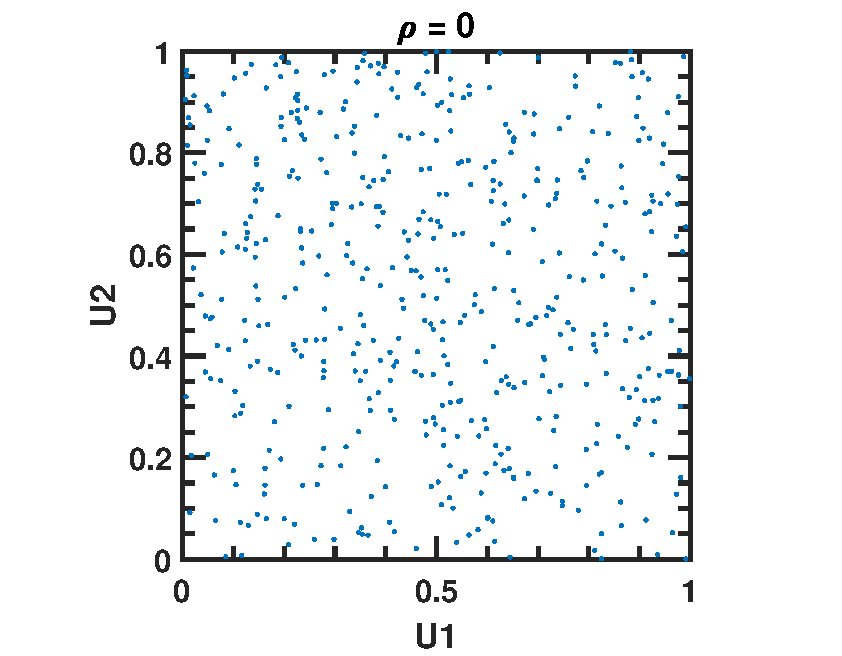
\includegraphics[width=\textwidth]{figures/statisticalModeling/GaussianCopulaDemo1}
			\end{subfigure}\quad
	\begin{subfigure}[b]{0.42\textwidth}
		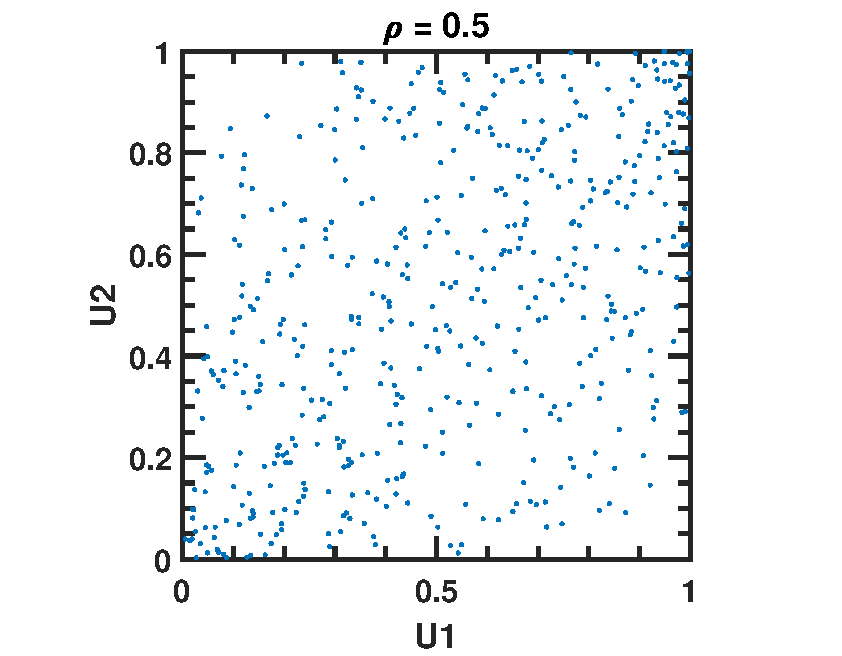
\includegraphics[width=\textwidth]{figures/statisticalModeling/GaussianCopulaDemo2}
	\end{subfigure}\quad
	\begin{subfigure}[b]{0.42\textwidth}
		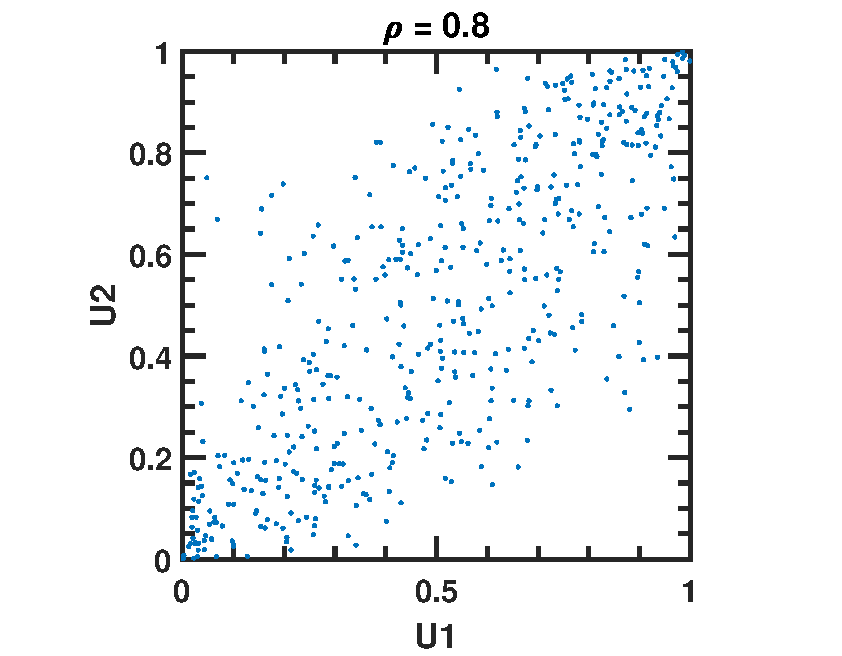
\includegraphics[width=\textwidth]{figures/statisticalModeling/GaussianCopulaDemo3}
		
	\end{subfigure}
		\begin{subfigure}[b]{0.42\textwidth}
		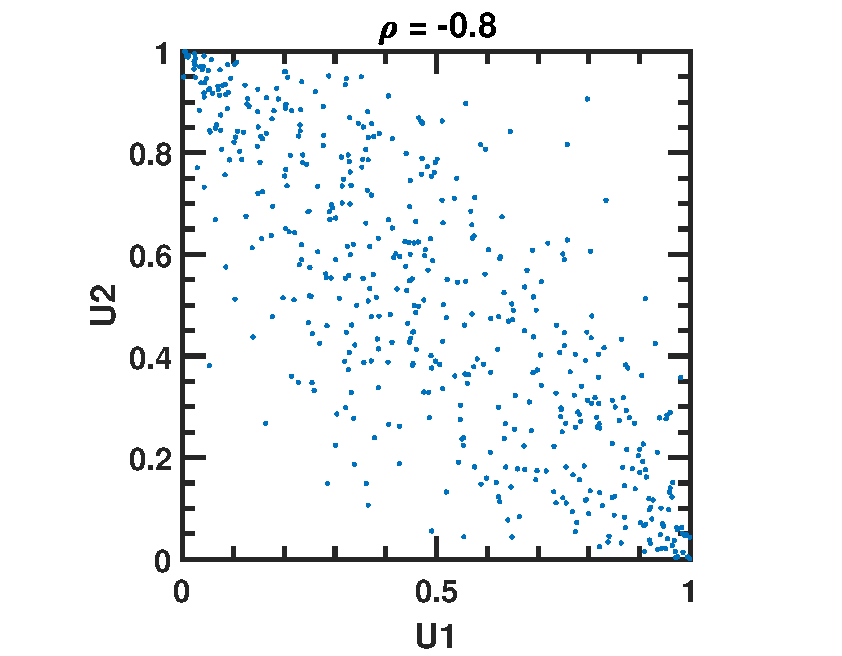
\includegraphics[width=\textwidth]{figures/statisticalModeling/GaussianCopulaDemo4}
		
	\end{subfigure}
	\caption{Gaussian copula with different correlations.}

\end{figure}


\begin{remark}[derivation of copula density function]
From \autoref{ch:statistical-models:SklarTheorem}, we know that	
$$c(x_1,...,x_d) = \frac{h(F_1(x_1),...,F_d(x_d))}{f_1(x_1)\cdots f_d(x_d)}.$$
Note that
$$h(x)= \frac{1}{(2\pi)^{d/2}\abs{det  R}^{1/2}}\exp(-\frac{1}{2}(x)^T R^{-1}(x)),x\in \R^d, $$
and
$$f_1\cdot f_2\cdots f_d= \frac{1}{(2\pi)^{d/2}}\exp(-\frac{1}{2}(x)^T (x)). $$
\end{remark}


\begin{lemma}[the copula associated with multivariate Gaussian distribution is Gaussian copula]\label{ch:statistical-models:th:CopulaOfMultivariateGaussian}\hfill
\begin{itemize}
	\item If $F$ is a multivariate normal distribution $MN(0,R)$, where $R$ is correlation matrix and $\Sigma = R$(that is, the margins are standard normal such that covariance matrix is equal to correlation matrix); then the copula associated with $F$ is the Gaussian copula with correlation matrix $R$
	\item If $F$ is a multivariate normal distribution $MN(0,\Sigma)$, then the copula associated with $F$ is the Gaussian copula with correlation matrix $R = D^{-1/2}\Sigma D^{-1/2}, D = diag(\Sigma).$
	\item If $F$ is a multivariate normal distribution $MN(\mu,\Sigma)$, then the copula associated with $F$ is the Gaussian copula with correlation matrix $R = D^{-1/2}\Sigma D^{-1/2}, D = diag(\Sigma).$
\end{itemize}
\end{lemma}
\begin{proof}
(1)Straight forward(\autoref{ch:statistical-models:th:constructCopulaForJointDistribution}). 
(2)(3) Let $\Phi$ denote the joint cdf $MN(\mu, \Sigma)$ and $\phi_i$ the marginal cdf $N(\mu_i,\sigma_i^2)$.  Let $\Phi^S$ denote the joint cdf $MN(\mu, R)$ and $\phi_i^S$ the marginal cdf $N(0,1)$.

Then,
\begin{align*}
\Phi(u_1,u_2,...,u_d) &= \Phi^S(\frac{u_1 - \mu_1}{\sigma_1^2},\frac{u_2 - \mu_2}{\sigma_2^2},...,\frac{u_d - \mu_d}{\sigma_d}) \\
\phi_i(u_i) &= \phi^S_i(\frac{u_i - \mu_i}{\sigma_i}) \\
\phi_i^{-1}(u_1) &= \sigma_i(\phi^S_i)^{-1} + \mu_i 
\end{align*}

Therefore,
\begin{align*}
&\Phi(\phi^{-1}_i(u_1),\phi^{-1}_2(u_2),...,\phi^{-1}_2(u_d)) \\
=&\Phi^S((\phi^{-1}_i(u_1) - \mu_1)/\sigma_1,(\phi^{-1}_i(u_2) - \mu_2)/\sigma_2,...,(\phi^{-1}_i(u_d) - \mu_d)/\sigma_d) \\
=&\Phi^S((\phi^S_1)^{-1},(\phi^S_2)^{-1},...,(\phi^S_d)^{-1}) 
\end{align*}
\end{proof}


\begin{lemma}[construct a multivariate cdf from Gaussian copulas and margins]\label{ch:statistical-models:th:ConstructMultivariateCDFwithGaussianCopulaAndMargins}
	Consider $d$ random variables $X_1,X_2,...,X_d$ with $F_1,F_2,...,F_d$ being the univariate cdf.
	Let $C$ be a $d$ dimensional Gaussian copulas given by
	$$C(u_1,u_2,...,u_d; R) = \Phi(\phi^{-1}(u_1),\phi^{-1}(u_2),...,\phi^{-1}(u_d)),$$
	where $u_1,u_2,...,u_d \in [0,1]$, $\Phi$ is the cdf for a multivariate normal distribution with zero mean and covariance matrix $R$, $\phi$ is the cdf for a standard normal variable.
	
	Then the joint distribution for $X_1,X_2,...,X_d$ is given by
	$$F(x_1,x_2,...,x_n) = \Phi(\phi^{-1}(F_1(x_1)),\phi^{-1}(F_2(x_2)),...,\phi^{-1}(F_d(x_d)));$$
	and the joint density function is given by
	
	$$f(x)= \frac{1}{(2\pi)^{d/2}\abs{det  R}^{1/2}}\exp(-\frac{1}{2}(x)^T R^{-1}(x))f_1(x_1)f_2(x)\cdots f_d(x_d), $$
	where $$x=(\phi^{-1}(F_1(x_1)),\phi^{-1}(F_2(x_2)),...,\phi^{-1}(F_d(x_d))).$$
	and $f_1,f_2,...,f_d$ are the marginal densities of $X_1,X_2,...,X_n$.
\end{lemma}
\begin{proof}
	(1)See \autoref{ch:statistical-models:th:ConstructMultivariateDistributionFromCopulaAndMargins}.
	(2)See \autoref{ch:statistical-models:SklarTheorem}. 
\end{proof}

\begin{example}[Gaussian margin with Gaussian copula will give multivariate Gaussian]
Note that from \autoref{ch:statistical-models:SklarTheorem}, we know that the joint cdf can be constructed from margins $f_1,f_2,...,f_d$ and $c(u_1,u_2,...,u_d)$ via
$$h(x_1,...,x_d) = c(F_1(x_1),...,F_d(x_d))\cdot f_1(x_1)\cdots f_d(x_d).$$

Let $\phi(x)$ be the standard Gaussian cdf, then a Gaussian random variable $N(m,\sigma^2)$ has pdf given by $\phi(\frac{x-m}{\sigma})$.

Then,
\begin{align*}
h(x_1,...,x_d) &= c(F_1(x_1),...,F_d(x_d))\cdot f_1(x_1)\cdots f_d(x_d) \\
&= \frac{1}{\sqrt{det(R)}} \exp(-\frac{1}{2}
\begin{bmatrix}
\phi^{-1}(\phi(x_1-m_1/\sigma_1)) \\
\vdots\\
\phi^{-1}(\phi(x_d-m_d/\sigma_d))
\end{bmatrix}^T \cdot (R^{-1} - I) \begin{bmatrix}
\phi^{-1}(\phi(x_1-m_1/\sigma_1)) \\
\vdots\\
\phi^{-1}(\phi(x_d-m_d/\sigma_d))
\end{bmatrix})\\
&\frac{1}{(2\pi)^{d/2}}\exp(\begin{bmatrix}
(x_1-m_1/\sigma_1)) \\
\vdots\\
(x_d-m_d/\sigma_d))
\end{bmatrix}^T \cdot \begin{bmatrix}
(x_1-m_1/\sigma_1)) \\
\vdots\\
(x_d-m_d/\sigma_d))
\end{bmatrix}
)
)\\
&= \frac{1}{\sqrt{det(R)}} \exp(-\frac{1}{2}
\begin{bmatrix}
(x_1-m_1/\sigma_1) \\
\vdots\\
(x_d-m_d/\sigma_d)
\end{bmatrix}^T \cdot (R^{-1}) \begin{bmatrix}
(x_1-m_1/\sigma_1) \\
\vdots\\
(x_d-m_d/\sigma_d)
\end{bmatrix})
\frac{1}{(2\pi)^{d/2}}
\\
&= \frac{1}{\sqrt{det(R)}(2\pi)^{d/2}} \exp(-\frac{1}{2}
\begin{bmatrix}
(x_1-m_1/\sigma_1) \\
\vdots\\
(x_d-m_d/\sigma_d)
\end{bmatrix}^T \cdot (\Sigma^{-1}) \begin{bmatrix}
(x_1-m_1/\sigma_1) \\
\vdots\\
(x_d-m_d/\sigma_d)
\end{bmatrix})
\end{align*}
where $\Sigma^{-1} = D^{-1}R^{-1}D^{-1}$, $D = diag(\sigma_1,\sigma_2,...,\sigma_d)$.

\end{example}


\begin{example}[bivariate Gaussian copula]
	$$C_{\rho}(u,v) = \int_{-\infty}^{\Phi^{-1}(u)}\int_{-\infty}^{\Phi^{-1}(v)}\frac{1}{2\pi(1-\rho^2)^{1/2}}\exp(-\frac{x^2-2\rho x y + y^2}{2(1-\rho^2)}) dxdy$$
	where $\rho$ is the linear correlation coefficient.
\end{example}



\subsubsection{t copula}

\begin{definition}[t copula]\label{ch:statistical-models:def:tCopula}\cite[419]{roncalli2016lecture}
A t-copula 	characterized by correlation matrix $R\in [-1,1]^{n\times n}$ and degree of freedom parameter $v$ is the copula associated with the multivariate Student's t probability distribution
$$C(u_1,u_2,...,u_n;\rho,v) = T_n(T_v^{-1}(u_1),T_v^{-1}(u_2),...,T_v^{-1}(u_n);R,v).$$


\end{definition}


\begin{figure}[H]
	\centering
	\begin{subfigure}[b]{0.42\textwidth}
		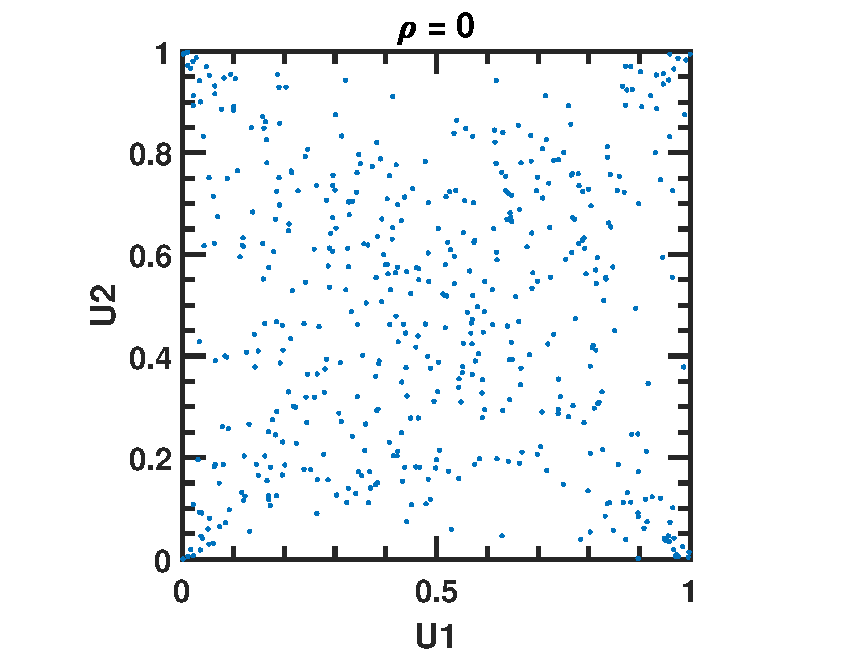
\includegraphics[width=\textwidth]{figures/statisticalModeling/StudentTCopulaDemo1}
	\end{subfigure}\quad
	\begin{subfigure}[b]{0.42\textwidth}
		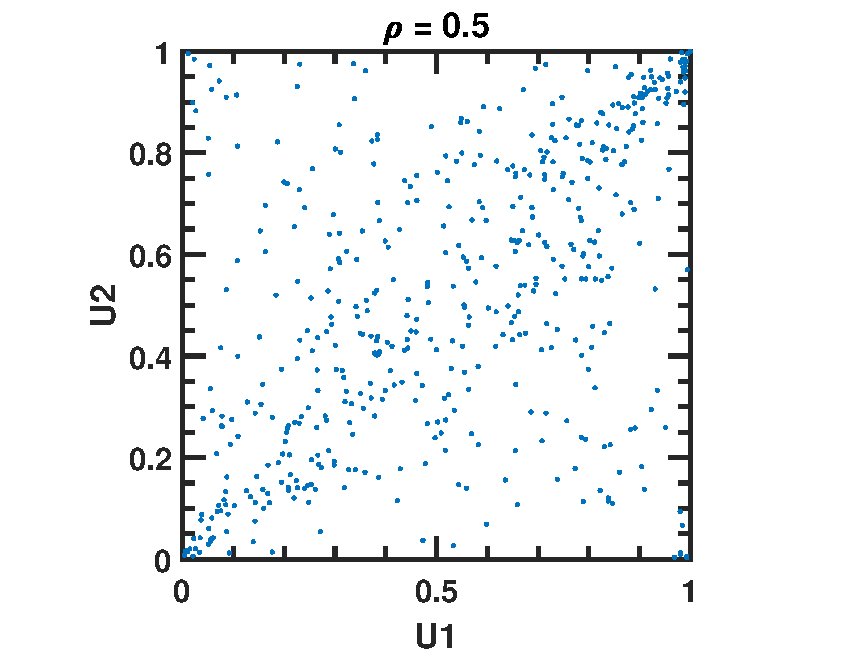
\includegraphics[width=\textwidth]{figures/statisticalModeling/StudentTCopulaDemo2}
	\end{subfigure}\quad
	\begin{subfigure}[b]{0.42\textwidth}
		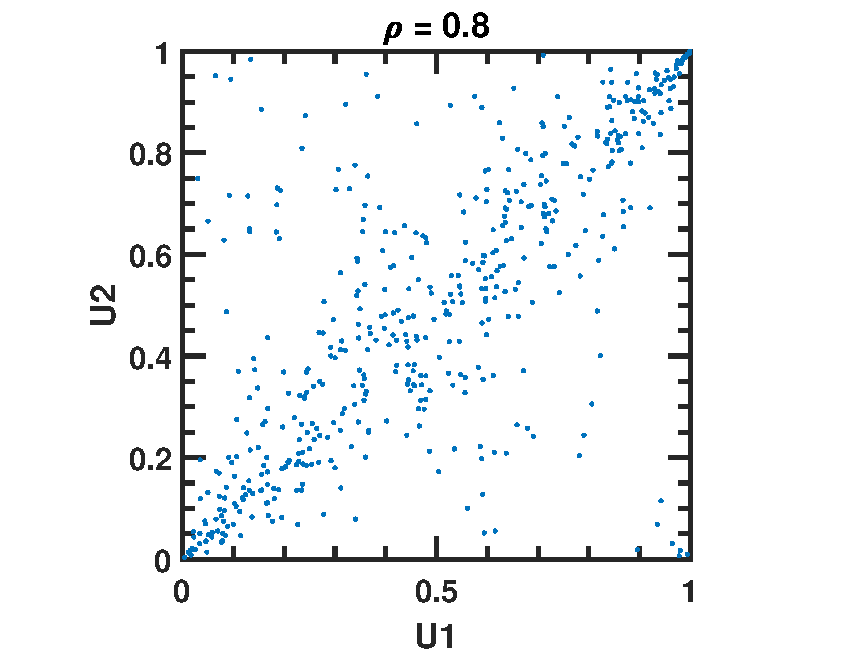
\includegraphics[width=\textwidth]{figures/statisticalModeling/StudentTCopulaDemo3}
		
	\end{subfigure}
	\begin{subfigure}[b]{0.42\textwidth}
		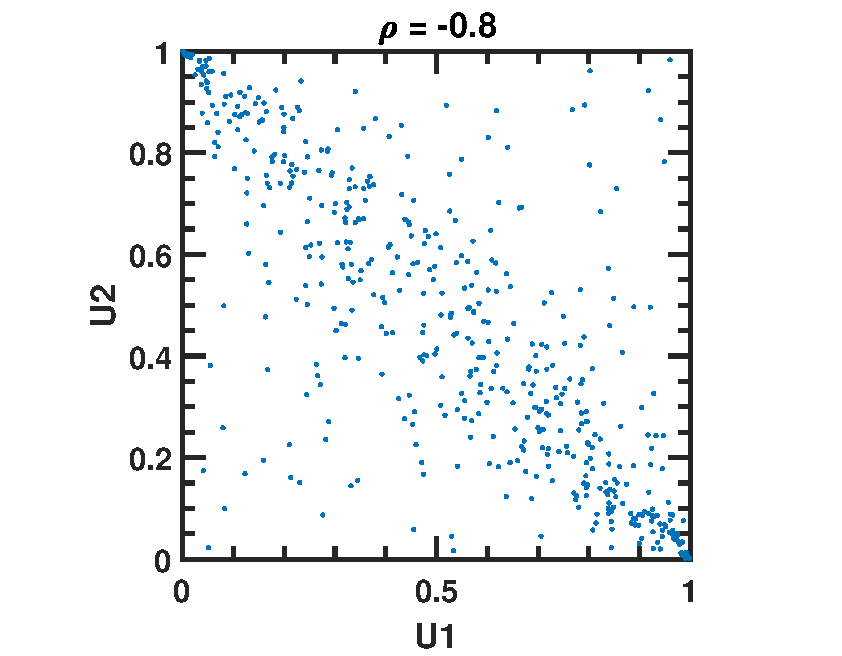
\includegraphics[width=\textwidth]{figures/statisticalModeling/StudentTCopulaDemo4}
		
	\end{subfigure}
	\caption{Student T copula with different correlations.}
	
\end{figure}


\begin{example}[bivariate t copula]
	$$C(u_1,u_2;\rho,v) = \int_{-\infty}^{T^{-1}_v(u_1)}\int_{-\infty}^{T^{-1}_v(u_2)}\frac{1}{2\pi(1-\rho^2)^{1/2}}(1 + \frac{x_1^2+x_2^2-2\rho x_1x_2}{v(1-\rho^2)})dx_1dx_2$$
	where $\rho$ is the linear correlation coefficient.
\end{example}

\cite{cherubini2004copula}

\subsubsection{Common copula functions: other copula}

\begin{definition}[product copula, co-monotonicity copula]\cite[187]{ruppert2015statistics}\cite[190]{mcneil2015quantitative}
	\begin{itemize}
		\item \textbf{(product copula, independence copula)}The d-dimensional product copula is given by
		$$C(u_1,u_2,...,u_d) = u_1u_2\cdots u_d, u_i\in [0,1],\forall i.$$
		The product copula corresponds to independence and it can be viewed as the cdf of $(U_1,...,U_d)$, where $U_1,...,U_d$ are independent uniform random variables.
		\item \textbf{(co-monotonicity copula)} The joint cdf of the random vector $(U_1,U_2,...,U_d)$, where $U$ is a uniform random variable is called a co-monotonicity copula, which characterizes perfect positive correlation. It is given by
		$$C(u_1,u_2,...,u_d) = \min(u_1,u_2,...,u_d).$$
		\item \textbf{two dimensional counter-monotonicity copula} is defined as the joint cdf of $(U,1-U)$.Therefore,
		\begin{align*}
		C(u_1,u_2) \triangleq &Pr(U\leq u_1,(1-U)\leq u_2) \\
		=& Pr(1-u_2\leq U\leq u_1) \\
		=& \max\{u_1+u_2-1,0\}
		\end{align*}
	\end{itemize}	
\end{definition}

\begin{remark}[interpretation]\cite[185]{ruppert2015statistics}\hfill
\begin{itemize}
	\item The co-monotonicity copula is the joint cdf of $\bm{U}=(U,U,...,U)$;that is, $\bm{U}$ contains $d$ copies of $U(0,1)$. The co-monotonicity copula is the upper bound of all copula functions(\autoref{ch:statistical-models:th:FrechetHoeffdingBounding}). 
	\item The two dimensional counter-monotonicity copula is the lower bound of all copula functions.
\end{itemize}
\end{remark}


\begin{definition}[t-copula]
\end{definition}

\subsection{Dependence and copula}

\subsubsection{Linear correlations}

\begin{example}
Consider discrete-valued random variable $V_1$ and $V_2$ given by: 
\begin{itemize}
	\item $V_1$ equally take three different values $-1,0,+ 1$.
	\item If $V_1 = -1 ~or~ + 1$, $V_2 = 1$. If $V_1= 0$, then $V_2 = 0$. 
\end{itemize}

It is clearly that $E[V_1V_2] = 0, E[V_1] = 0 \implies Cov[V_1,V_2] = 0$; however, it is clearly that $V_1$ and $V_2$ are uncorrelated but they are dependent since 
$$Pr(V_2|V_1 = v) \neq Pr(V_2).$$
where $$Pr(V_2 = 1) = Pr(V_2 = 1|V_1 = 1)Pr(V_1 = 1) + Pr(V_2 = 1|V_1 = 1)Pr(V_1 = 1) = 1\times 1/3 + 1\times 1/3 = 2/3;$$
and
$$Pr(V_2 = 0) = Pr(V_2 = 0|V_1 = 0)Pr(V_1 = 0) = 1\times 1/3= 1/3.$$
\end{example}



\begin{definition}[linear correlation, Pearson correlation]\cite[202]{mcneil2015quantitative}\index{linear correlation}\index{Person correlation}
Given two random variables $X$ and $Y$. The linear correlation is defined by	
	$$\rho(X,Y) = \frac{Cov(X,Y)}{\sqrt{Var[X]Var[Y]}}.$$
\end{definition}



\begin{note}[characteristics of linear correlations]\hfill
\begin{itemize}
	\item sensitive to outliers.
	\item measure the 'average dependence' between $X$ and $Y$.
	\item invariant under strictly \textbf{increasing linear transformation}.
	\item May be misleading when multivariate distribution is not elliptical.
\end{itemize}
\end{note}


\begin{lemma}[invariance of correlation under affine transformation]\label{ch:statistical-models:th:CorrelationInvarianceUnderAffineTransformation}\hfill
\begin{itemize}
	\item Let random variables $X$ and $Y$ have correlation $\rho(X,Y)$. Then
	$$\rho(aX+b, cY + d) = \rho(X,Y), \forall a,c >0, b,d\in \R.$$
	\item Let random variables $X$ and $Y$ have correlation $\rho(X,Y)$. Then
	$$\rho(aX+b, cY + d) = \frac{cd}{\abs{cd}}\rho(X,Y), \forall a,b, b,d\in \R.$$
\end{itemize}	
	
\end{lemma}
\begin{proof}
(1)	
$$\rho(aX+b, cY + d) \triangleq  \frac{Cov(aX + b,cY + d)}{\sqrt{Var[aX+b]Var[cY+d]}} = \frac{aCov(X,Y)d}{\sqrt{a^2Var[X]Var[Y]c^2}} = = \rho(X,Y). $$	
(2) straight forward.
\end{proof}

\begin{remark}[generally not invariant under nonlinear transformation]
Let $T:\R \to \R$ be a nonlinear strictly increasing function. Then generally $$\rho(X,Y) \neq \rho(T(X), T(Y)).$$	
\end{remark}


\begin{lemma}[perfect linear correlation and linear function relationship]\label{ch:statistical-models:th:PerfectLinearCorrelationAndLinearFunctionRelationship}\cite[202]{mcneil2015quantitative} Let $X$ and $Y$ be two random variable defined on the same probability space.  It follows that
\begin{itemize}
	\item $\rho(X,Y) = 1$ implies $Y = \alpha  + \beta X$ almost surely for some $\alpha,\beta \in \R, \beta >0$.
	\item $\rho(X,Y) = -1$ implies $Y = \alpha  + \beta X$ almost surely for some $\alpha,\beta \in \R, \beta <0$.
	\item Conversely, if $Y = \alpha + \beta X$, then $\rho(X,Y) = sign(\beta)$.
\end{itemize}	
\end{lemma}
\begin{proof}
(1)(2) Note that the equality holds only when the equality holds in Cauchy inequality(\autoref{ch:theory-of-probability:th:Cauchy-SchwarzInequality}).Then, $X$ and $Y$ must have linear dependence almost everywhere. 
(3)  Use the affine transformation invariance property of correlation(\autoref{ch:statistical-models:th:CorrelationInvarianceUnderAffineTransformation}),
\end{proof}

\subsubsection{Rank correlations}

\begin{definition}[Kendall's tau for observations]\label{ch:statistical-models:th:KendallTauForObservations}\hfill
\begin{itemize}
	\item Let $(x_1,y_1),(x_2,y_2),...,(x_n,y_n)$ be a set of joint observations from two random variables $X$ and $Y$.
	\item A pair of observations $(x_i,y_i)$ and $(x_j,y_j)$ are \textbf{concordant} if both $x_i > x_j$ and $y_i>y_j$ or if both $x_i < x_j$ and $y_i<y_j$; 
	\item They are \textbf{discordant}, if $x_i > x_j$ and $y_i<y_j$ or if $x_i < x_j$ and $y_i>y_j$. 
	\item If $x_i=x_j, y_i=y_j$, the pair is neither concordant nor discordant.
	\item The \textbf{Kendall $\tau$ coefficient} is defined as
	$$\rho_\tau = \frac{num ~concordant~pairs - num ~disconcordant~pairs}{n(n-1)/2}.$$
\end{itemize}	
Note that $n(n-1)/2$ is the total number of pairs to compare.
\end{definition}


\begin{definition}[Kendall's tau for random variables]\index{Kendall's tau}\cite[207]{mcneil2015quantitative}
Let $X_1$ and $X_2$ be two random variables. Then the Kendall's tau is given by
$$\rho_\tau = E[sign((X_1-\tilde{X}_1)(X_2 - \tilde{X}_2))],$$
where $(\tilde{X}_1,\tilde{X}_2)$ is a independent copy of $(X_1,X_2)$; that is,$(\tilde{X}_1,\tilde{X}_2)$ has the same cdf of $(X_1,X_2)$, but they are statistically independent. 	
\end{definition}




\begin{lemma}[Kendall's tau from copula]\cite[207]{mcneil2015quantitative}\label{ch:statistical-models:KendallTauFromCopula}
The $C$ be the copula associated with the joint cdf of $(X,Y)$, then 
\begin{align*}
\rho_{\tau}(X,Y) & = 4\int_0^1\int_0^1 C(u,v)dC(u,v) - 1 \\
&=4E[C(U,V)] - 1
\end{align*}
\end{lemma}
\begin{proof}
From the definition 
\begin{align*}
\rho_\tau &= E[sign((X_1-\tilde{X}_1)(X_2 - \tilde{X}_2))] \\
& =E[\bm{1}((X_1-\tilde{X}_1)(X_2 - \tilde{X}_2)>0)]-E[\bm{1}((X_1-\tilde{X}_1)(X_2 - \tilde{X}_2)<0)] \\
&=Pr((X_1-\tilde{X}_1)(X_2 - \tilde{X}_2)>0)-Pr((X_1-\tilde{X}_1)(X_2 - \tilde{X}_2)<0) \\
&=2Pr((X_1-\tilde{X}_1)(X_2 - \tilde{X}_2)>0) - 1\\
&=2Pr((X_1-\tilde{X}_1)>0,(X_2 - \tilde{X}_2)>0) + 2Pr((X_1-\tilde{X}_1)<0,(X_2 - \tilde{X}_2)<0)- 1 \\
&=4Pr((X_1-\tilde{X}_1)<0,(X_2 - \tilde{X}_2)<0) - 1 \\
&=4\int_{-\infty}^{\infty}\int_{-\infty}^{\infty}Pr((X_1<s_1,X_2 <s_2)f_{\tilde{X}_1,\tilde{X}_2}(s_1,s_2)ds_1ds_2 - 1 \\
&=4\int_{-\infty}^{\infty}\int_{-\infty}^{\infty}F(s_1,s_2)dF(s_1,s_2) - 1 \\
&=4\int_{-\infty}^{\infty}\int_{-\infty}^{\infty}C(F_1(s_1),F_2(s_2))dC(F_1(s_1),F_2(s_2)) - 1 \\
&=4\int_{0}^{1}\int_{0}^{1}C(u_1,u_2)dC(u_1,u_2) - 1
\end{align*}

\end{proof}

\begin{remark}[Kendall's tau is independent of the marginal cdf]
Note that Kendall's tau only depends on the correlation structure characterized by the copula; it is independent of the marginal cdf.	
\end{remark}


\begin{lemma}[Hoffding formula for covariance]\cite[204]{mcneil2015quantitative}\label{ch:statistical-models:th:HoffdingFormuaForCovariance}
If $(X_1,X_2)$ has joint cdf $F$ and marginal cdf $F_1$ and $F_2$, then
\begin{itemize}
	\item $$Cov(X_1,X_2) = \frac{1}{2}E[(X_1-\tilde{X}_1)(X_2 - \tilde{X}_2)],$$
	where $(\tilde{X}_1,\tilde{X}_2)$ is a independent copy of $(X_1,X_2)$; that is,$(\tilde{X}_1,\tilde{X}_2)$ has the same cdf of $(X_1,X_2)$, but they are statistically independent. 
	\item $$Cov(X_1,X_2) = \int_{-\infty}^{\infty}\int_{-\infty}^{\infty} (F(x_1,x_2) - F_1(x_1)F_2(x_2))dx_1dx_2.$$
\end{itemize}
\end{lemma}
\begin{proof}
(1) Directly expand the rhs. Note that $E[X_1\tilde{X}_2] = E[X_1]E[\tilde{X}_2]$ due to independence.
(2)
A useful identity is for any $a\in \R,b\in R$, we have
$$(a-b) = \int_{-\infty}^{\infty} H(x-b) - H(x-a) dx.$$

We have
\begin{align*}
&E[(X_1-\tilde{X}_1)(X_2 - \tilde{X}_2)] \\
=& E[\int_{-\infty}^{\infty} \int_{-\infty}^{\infty} (H(s_1-X_1) - H(s_1-\tilde{X}_1))(  H(s_2-X_2) - H(s_2-\tilde{X}_2)) ds_1ds_2]\\
=&\int_{-\infty}^{\infty} \int_{-\infty}^{\infty} E[(H(s_1-X_1) - H(s_1-\tilde{X}_1))(  H(s_2-X_2) - H(s_2-\tilde{X}_2))] ds_1ds_2 \\
=&2\int_{-\infty}^{\infty} \int_{-\infty}^{\infty} Pr(X_1\leq s_1,X_2\leq s_2) - Pr(X_1\leq s_1)Pr(X_2\leq s_2)ds_1ds_2\\
=&2\int_{-\infty}^{\infty}\int_{-\infty}^{\infty} (F(s_1,s_2) - F_1(s_1)F_2(s_2))ds_1ds_2
\end{align*}
\end{proof}




\begin{definition}[Spearman's rho]\index{Spearman's rho}\cite[207]{mcneil2015quantitative}
Let $X_1$ and $X_2$ be two random variables with marginal cdf $F_1$ and $F_2$. \textbf{Spearman's rho} is defined as
	$$\rho_{S}(X,Y)  = \rho(F_1(X_1),F_2(X_2)).$$
In other words, Spearman's rho is the linear correlation of the transform random variables.	
\end{definition}


\begin{definition}[Spearman's rho for observations]\index{Spearman's rho}\label{ch:statistical-models:def:SpearmanRhoFromObservations}\hfill
\begin{itemize}
	\item Let $(x_1,y_1),(x_2,y_2),...,(x_n,y_n)$ be a set of joint observations from two random variables $X$ and $Y$.
	\item Let $R(x_i)$ denote the rank of $x_i$ among $x_1,x_2,...,x_n$, where $R(x_i)$ will take value from 1 to n. Similarly we denote $R(y_i)$ as the rank of $y_i$. 
	\item The \textbf{Spearman's $\rho$ coefficient} is defined as
	$$\rho_S = \frac{\frac{1}{n}\sum_{i=1}^n (R(x_i) - \bar{R}(x))(R(y_i) - \bar{R}(y))}{\sqrt{\frac{1}{n}\sum_{i=1}^n (R(x_i) - \bar{R}(x))^2\frac{1}{n}\sum_{i=1}^n (R(y_i) - \bar{R}(y))^2 }},$$
	where $\bar{R}(y) = \frac{1}{n}\sum_{i=1}^n R(y_i)$.
	\item It can be showed that 
	$$\rho_S = 1 - \frac{\sum_{i=1}^{n}(R(x_i) - R(y_i))^2}{n^3-n}.$$
\end{itemize}	
\end{definition}

\begin{lemma}[properties of Spearman's rho for observations]
Let $(x_1,y_1),(x_2,y_2),...,(x_n,y_n)$ be a set of joint observations from two random variables $X$ and $Y$. It follows that
\begin{itemize}
	\item $$n\bar{R}(y) = \sum_{i=1}^n R(y_i) = \frac{1}{2}n(n+1).$$
	\item $$\sum_{i=1}^n R(y_i)^2 = \sum_{i=1}^n R(x_i)^2 = \frac{n(n+1)(2n+1)}{6}.$$
	\item $$\rho_S = 1 - \frac{\sum_{i=1}^{n}(R(x_i) - R(y_i))^2}{n^3-n}.$$
\end{itemize}	
\end{lemma}
\begin{proof}
(1)straight forward.(2) this is the sum of squares from 1 to n. (3)
Note that
$$\sum_{i=1}^n (R(x_i) - \bar{R}(x))^2 = \sum_{i=1}^n R(x_i)^2 - (\sum_{i=1}^n R(x_i))^2 = \frac{n(n+1)(2n+1)}{6} - (\frac{1}{2}n(n+1))^2.$$
and
$$\sum (R(x_i) - R(y_i))^2 = \sum R(x_i)^2 + \sum R(y_i)^2 - 2\sum R(x_i)R(y_i)$$
implies 
$$2\sum R(x_i)R(y_i) =\sum R(x_i)^2 + \sum R(y_i)^2 - \sum (R(x_i) - R(y_i))^2. $$ 	
\end{proof}

\begin{lemma}[Spearman's rho from copula]\cite[207]{mcneil2015quantitative}\label{ch:statistical-models:th:SpearmanRhoFromCopula}
\begin{align*}
\rho_{S}(X,Y) = 12\int_0^1\int_0^1 C(u,v)dudv - 3
\end{align*}	
\end{lemma}
\begin{proof}
From definition and use \autoref{ch:statistical-models:th:HoffdingFormuaForCovariance}, we have
\begin{align*}
\rho_{S}(X,Y)  &= \rho(F_1(X_1),F_2(X_2)) \\
& = Cov(F_1(X_1),F_2(X_2))/(\sqrt{Var[F_1[X_1]]Var[F_2[X_2]]}) \\
& = 12 Cov(F_1(X_1),F_2(X_2)) \\
& = 12 \int_{-\infty}^{\infty}\int_{-\infty}^{\infty} \hat{F}(F_1(x_1),F_2(x_2)) - \hat{F}_1(F_1(x_1))\hat{F}_2(F_2(x_2)) dx_1dx_2\\
& = 12 \int_{-\infty}^{\infty}\int_{-\infty}^{\infty} \hat{F}(F_1(x_1),F_2(x_2)) - x_1x_2 dx_1dx_2 \\
& = 12(\int_0^1\int_0^1 C(u,v)dudv - \frac{1}{4})
\end{align*}	
where we use the property $F_1(X_1),F_2(X_2)$ are uniform random variable with variance 1/12, and the joint cdf of $(F_1(X_1),F_2(X_2))$ is the copula associated with joint cdf of $(X_1,X_2)$( 
\autoref{ch:statistical-models:th:ProbababilityTransformForRandomVectorAndProperties}).
\end{proof}


\begin{lemma}[Spearman's rho for monotonic relation]
Let $X$ be a random variable and let $Y$ be a monotonic function of $X$, denoted by $Y = f(X)$. It follows that
\begin{itemize}
	\item If $f$ is a monotonically increasing function, the $\rho_S(X,Y) = 1.$
	\item If $f$ is a monotonically decreasing function, the $\rho_S(X,Y) = -1.$
\end{itemize}	
\end{lemma}
\begin{proof}
(1)Consider the Spearman's rho for observations(\autoref{ch:statistical-models:def:SpearmanRhoFromObservations}). For each sample $(x_i,y_i)$, each component has the same rank.	
(2)For each sample $(x_i,y_i)$, each component has ranks satisfying
$$R(x_i) - \bar{R}(x_i) = -(R(y_i) - \bar{R}(y_i)).$$	

\end{proof}



\begin{lemma}[first quadrant probability of bivariate Gaussian distribution]\cite[215]{mcneil2015quantitative}\label{ch:statistical-models:th:FirstQuadrantProbabilityBivariateGaussain}
Let $(X_1,X-2)$ be a random vector with joint multivariate Gaussian distribution $MN(0,\Sigma)$. Let $\rho = \rho(X_1,X_2)$. Then
$$Pr(X_1>0, X_2>0) = \frac{1}{4}+ \frac{\arcsin \rho}{2\pi}.$$	
\end{lemma}
\begin{proof}
See reference. 
\end{proof}

\begin{lemma}[rank correlation for Gaussian copula]\cite[215]{mcneil2015quantitative}\label{ch:statistical-models:th:RankCorrelationGaussianCopula}
Let $(X_1,X_2)$ be a bivariate random vector with Gaussian copula characterized by correlation coefficient $\rho$ and continuous margins. Then
\begin{itemize}
	\item $$\rho_\tau(X_1,X_2) = \frac{2}{\pi}\arcsin \rho$$	
	\item $$\rho_S(X_1,X_2) = \frac{6}{\pi}\arcsin \frac{1}{2}\rho$$	
\end{itemize}	
\end{lemma}
\begin{proof}
(1) Note that Kendall's tau only depends on the copula; therefore we can assume $(X_1,X_2)$ has bivariate normal distribution($MN(0,2\Sigma)$, correlation $\rho$). From \autoref{ch:statistical-models:KendallTauFromCopula},
\begin{align*}
\rho_\tau &= 4Pr((X_1-\tilde{X}_1)>0,(X_2 - \tilde{X}_2)>0) - 1 \\
&=4Pr(Y_1>0,Y_2>0) - 1 \\
&=4(\frac{1}{4}+ \frac{\arcsin \rho}{2\pi}) - 1\\
&=\frac{2}{\pi}\arcsin \rho
\end{align*}
where $(\tilde{X}_1,\tilde{X}_2)$ is the independent copy of $(X_1,X_2)$, and $Y_1 = X_1-\tilde{X_2}\sim MN(0,2\Sigma)$($Y_1$ has the same correlation $\rho$), we use \autoref{ch:statistical-models:th:FirstQuadrantProbabilityBivariateGaussain}.
(2) From \autoref{ch:statistical-models:th:SpearmanRhoFromCopula}, we have
\begin{align*}
\rho_S(X_1,X_2) &= 12\int_0^1\int_0^1 C(u,v)dudv - 3 \\
&=12\int_0^1\int_0^1 \Phi(\phi^{-1}(u),\phi^{-1}(v))dudv - 3 \\
&=12\int_{-\infty}^{\infty}\int_{-\infty}^{\infty} \Phi(s_1,s_2)d\phi(s_1)d\phi(s_2) - 3 \\
&=12\int_{-\infty}^{\infty}\int_{-\infty}^{\infty} \Phi(s_1,s_2) f(s_1)f(s_2)ds_1ds_2 - 3 \\
&=12 Pr(X_1-S_1<0, X_2-S_2<0) -3 \\
&=12 Pr(Y_1<0,Y_2<0) -3 \\
&=12(\frac{1}{4}+ \frac{\arcsin \rho/2}{2\pi}) - 3\\
&=\frac{6}{\pi}\arcsin \frac{1}{2}\rho
\end{align*}
where $(\tilde{X}_1,\tilde{X}_2)$ is the independent copy of $(X_1,X_2)$, and $Y_1 = X_1-S_1\sim MN(0,\Sigma + I_2)$($Y_1$ has the correlation $\rho/2$), we use \autoref{ch:statistical-models:th:FirstQuadrantProbabilityBivariateGaussain}.
\end{proof}


\begin{remark}[applications in robust correlation estimation for multivariate Gaussian random variables]
Note that multivariate Gaussian distribution has Gaussian copula(\autoref{ch:statistical-models:th:CopulaOfMultivariateGaussian}). Therefore, we can estimate $\rho_\tau, \rho_S$ first(which is robust) and then convert them to linear correlation coefficients.	
\end{remark}



\subsubsection{Tail dependence}

\begin{definition}[tail dependence]
Let $X$ and $Y$ be random variables with marginal cdf $F_X$ and $F_Y$.
\begin{itemize}
	\item The \textbf{coefficient	of upper tail dependence} of $X$ and $Y$ is
	\begin{align*}
	\lambda_u(X,Y) \triangleq &= \lim_{\alpha\to 1} Pr(F_Y(Y) > \alpha | F_X(X) > \alpha) \\
	&= \lim_{\alpha\to 1} Pr(Y > F^{-1}_Y(\alpha)|X > F^{-1}_X(\alpha)).
	\end{align*}
	\item The \textbf{coefficient	of lower tail dependence} of $X$ and $Y$ is
	\begin{align*}
	\lambda_l(X,Y) \triangleq &= \lim_{\alpha\to 0} Pr(F_Y(Y) \leq \alpha | F_X(X) \leq \alpha) \\
	&= \lim_{\alpha\to 0} Pr(Y > F^{-1}_Y(\alpha)|X > F^{-1}_X(\alpha)).
	\end{align*}
\end{itemize}
 

Tail dependence is the probability of observing a large(small) $Y$ given that $X$ is large(small). If $\lambda_u > 0(\lambda_l > 0)$, then we say $(X,Y)$ has an upper(lower) tail dependence. 
\end{definition}

\begin{lemma}[tail dependence from copula]\hfill
\begin{itemize}
	\item 
	$$\lambda_l = \lim_{q\to 0^+} \frac{ Pr(F_Y(Y) \leq q , F_X(X) \leq q)}{Pr(F_X(X) \leq q)} = \lim_{q\to 0^+} \frac{C(q,q)}{q}.$$
	\item 
	$$\lambda_u = \lim_{q\to 1^-} \frac{ Pr(F_Y(Y) > q , F_X(X) > q)}{Pr(F_X(X) > q)} = \lim_{q\to 1^-} \frac{C^s(q,q)}{1-q},$$
	where $C^s$ is the survival copula.
\end{itemize}	
\end{lemma}

\begin{remark}[tail dependence is independent of the marginal cdf]\hfill
\begin{itemize}
	\item 	Note that tail dependence only depends on the correlation structure characterized by the copula; it is independent of the marginal cdf.
	\item The existence of tail will depend on margins.
\end{itemize}	
	
\end{remark}


\begin{lemma}[tail independence of Gaussian copula]
Let $(X,Y)$ be a bivariate random vector with Gaussian copula characterized by correlation coefficient $\rho$ and continuous margins.	Then
	$$\lambda_u=\lambda_l = 2\lim_{x\to \infty} \Phi(x\sqrt{1-\rho}/\sqrt{1+\rho}) = 0.$$
\end{lemma}
\begin{proof}
From definition, we have
\begin{align*}
\lambda_l &= \lim_{q\to 0^+} \frac{ Pr(F_Y(Y) \leq q , F_X(X) \leq q)}{Pr(F_X(X) \leq q)} \\
&=\lim_{q\to 0^+} \frac{ Pr(Y \leq f^{-1}(q) , X \leq \phi^{-1}(q))}{Pr(X \leq f^{-1}(q))} \\
&=\lim_{q\to -\infty} \frac{ Pr(Y \leq q , X \leq q)}{Pr(X \leq q)} \\
&=\lim_{q\to -\infty} \frac{ Pr(Y \leq q , X \leq q)}{Pr(X \leq q)} \\
&= \lim_{q\to -\infty} \frac{ \int_{-\infty}^{q}\int_{-\infty}^{q} f(x,y)dxdy}{\int_{-\infty}^{q} f(x)dx} \\
&=\lim_{q\to -\infty} \frac{ \int_{-\infty}^{q}f(x,q)dx}{ f(q)} + \frac{ \int_{-\infty}^{q}f(q,y)dy}{ f(q)} \\
&=2\lim_{q\to -\infty} \frac{ \int_{-\infty}^{q}f(x,q)dx}{ f(q)} \\
&=2\lim_{q\to -\infty} f(x|y=q)dx
\end{align*}
where $f(x,y)$ is the density of $(X,Y)$, $f(x)$ is the marginal density, and we use L'hospital rule in the derivation.  
Note that $X|y=q \sim N(\rho q, 1-\rho^2)$(\autoref{ch:theory-of-statistics:th:multivariatenormalconditionaldistribution}); therefore, 
$$\lim_{q\to -\infty} f(x|y=q)dx = \Phi(\frac{q-\rho q}{\sqrt{1-\rho^2}}).$$
\end{proof}

\subsection{Estimating copula function}
\subsubsection{Empirical copula method}


\begin{definition}[empirical copula]\cite[424]{roncalli2016lecture}
Suppose we have observation of $n$ iid $d$ dimensional random vectors, $$X^i = (X_1^{(i)},X_2^{(i)},...,X_d^{(i)}),i=1,2,...,n,$$
We can construct its empirical copula associated with the joint distribution of $X$ via the following procedures:	
	\begin{itemize}
		\item (construct empirical marginal cdf)
		$$\hat{F}_k(x) = \frac{1}{n}\sum_{i=1}^{n}\bm{1}(X^{(i)}_k\leq x), k=1,2,...,d$$
		\item (construct transformed uniform sample)
		$$(\hat{U}_1^{(i)},...,\hat{U}_d^{(i)}) = (\hat{F}_1(X_1^i),...,\hat{F}_d(X_d^{(i)})),i=1,...,n$$
		\item (construct empirical copula)$$\hat{C}(u_1,u_2,...,u_d) = \frac{1}{n}\sum_{i=1}^n \bm{1}(\hat{U}_1^{(i)} \leq u_1,...,\hat{U}_1^{(i)} \leq u_d)$$
	\end{itemize}	
\end{definition}


\begin{remark}
	The nature of copula is the cdf of the transformed uniform random vector $(F_1(X_1),F_2(X_2),...,F_n(X_n))$(\autoref{ch:statistical-models:th:ProbababilityTransformForRandomVectorAndProperties}).
\end{remark}


\subsubsection{Maximum likelihood method}


\begin{lemma}[maximum likelihood function and two-stage estimation method]\cite[429]{roncalli2016lecture}
Suppose we have observation of $n$ iid $d$ dimensional random vectors, $$X^i = (X_1^{(i)},X_2^{(i)},...,X_d^{(i)}),i=1,2,...,n.$$
Assume the joint cdf for $X$ is given by
$$F(x_1,x_2,...,x_n) = C(F_1(x_1;\theta_1),...,F_d(x_d;\theta_d)),$$
such that we have two sets of parameters given by
\begin{itemize}
	\item $(\theta_1,...,\theta_d)$ for univariate distribution function $F_1,F_2,...,F_d$;
	\item $\theta_c$ for the copula function $C(u_1,...,u_d)$.
\end{itemize}	
\end{lemma}

The maximum log likelihood function is given by
\begin{align*}
&l(\theta_1,...,\theta_d,\theta_c) \\
&
= \sum_{i=1}^{n} \ln c(F_1(x^{(j)}_1;\hat{\theta}_1),...,F_1(x^{(j)}_d;\hat{\theta}_d) + 
\sum_{i=1}^{n}\sum_{j=1}^{d} 
\end{align*}
The first stage is to estimate univariate parameter $\theta_1,...,\theta_d$ via
$$\hat{\theta}_i = \arg\max \sum_{j=1}^{N} \ln f_i(x^{(j)}_i;\theta_i).$$

The second stage is to estimate the copula parameters $\theta_c$ with the estimated univariate parameters $\hat{\theta}_1,\hat{\theta}_2,...,\hat{\theta}_d$ fixed via
$$\hat{\theta}_c = \arg\max \sum_{j=1}^{N} \ln c(F_1(x^{(j)}_1;\hat{\theta}_1),...,F_1(x^{(j)}_d;\hat{\theta}_d);\theta_c).$$

\subsection{Applications of copula}

\subsubsection{Generating correlated uniform random number}

\begin{lemma}[conditional method for generating bivariate uniform random number with arbitrary joint distribution]\cite[96]{schmitz2003copulas}
Suppose that we want to generate a pair of random variables with marginal uniform $U(0,1)$ and joint cdf given by copula $C(u,v)$. 

We use the following procedures:
\begin{itemize}
	\item Generate $U$ and $T$ independently from $U(0,1)$; 
	\item Set $V = C_u^{-1}(T)$, where
	$C_u = \frac{\Pa}{\Pa u}C(u,v).$
	\item The desired pair is $(U,V)$.
\end{itemize}	
\end{lemma}
\begin{proof}
Note that (\autoref{ch:statistical-models:th:partialDifferentialCopulaGivesConditionalDistributionForUniformRandomVariables})
$$C_u = \frac{\Pa}{\Pa u}C(u,v) = Pr(V<v|U=u),$$
which is the conditional cdf. Then we use inverse transformation method to get $V$.
\end{proof}


\begin{lemma}[conditional method for generating bivariate uniform random number with arbitrary joint distribution]\cite[96]{schmitz2003copulas}
	
	Suppose that we want to generate a set of $n$ random variables with marginal uniform $U(0,1)$ and joint cdf given by copula $C_n(u_1,u_2,...,u_n)$.
	
	Further denote $C_{1:k}(u_1,...,u_k)$ be the copula of $(U_1,U_2,...,U_k), 2\leq k\leq n$ and set $C_1(u_1) = u_1$. 
	
	We use the following procedures:
	\begin{itemize}
		\item Simulate $u_1$ from $U(0,1)$.
		\item Simulate $u_2$ from the conditional distribution function $C_2(u_2|u_1)$.
		\item Simulate $u_3$ from the conditional distribution $C_3(u_3|u_1,u_2)$.
		\item $\cdots$
		\item Simulate $u_n$ from the conditional distribution $C_n(u_n|u_1,u_2,...,u_{n-1})$.
	\end{itemize}	
where
\begin{align*}
C_k(u_k|u_1,...,u_{k-1}) &\triangleq Pr(U_k\leq u_k|U_1=u_1,...,U_{k-1}=u_{k-1}) \\
&=\frac{\frac{\Pa^{k-1}}{\Pa u_1 ... \Pa u_{k-1}} C_{1:k}(u_1,...,u_k)}{\frac{\Pa^{k-1}}{\Pa u_1 ... \Pa u_{k-1}} C_{1:k-1}(u_1,...,u_k-1)}
\end{align*}
\end{lemma}
\begin{proof}
See \autoref{ch:statistical-models:th:partialDifferentialCopulaGivesConditionalDistributionForUniformRandomVariables} for how partial derivative is associated with conditional distribution.	
\end{proof}


\begin{lemma}[generate correlated uniform random variables with Gaussian copula correlation structure]
	Given a Gaussian copula $C$ characterized by correlation matrix  $\Sigma$. 	
	We can generate random vector $(X_1,X_2,...,X_n)$ with uniform distribution and Gaussian copula correlation structure  using the following procedures:
	\begin{itemize}
		\item First generate $(Y_1,Y_2,...,Y_n) \sim MN(0,\Sigma)$.
		\item Then transform $X_1 = \phi(Y_1),X_2 = \phi(Y_2),...,X_n = \phi(Y_n)$, where $\phi$ is standard normal cdf.
	\end{itemize}

\end{lemma}
\begin{proof}
	Note that $Y_1,Y_2$ alone is standard normal variable. Therefore $\phi(Y_1)$ and $\phi(Y_2)$ are uniform random variables(\autoref{ch:statistical-models:th:probabilityintegraltransform}). 
	To show $C$ is the copula associated with the cdf $F$, we have
	\begin{align*}
	F(x_1,x_2) &= Pr(X_1\leq x_1, X_2\leq x_2) \\
	&= Pr(\phi(Y_1) \leq x_1, \phi(Y_2) \leq x_2) \\
	&=Pr(\phi(Y_1) \leq x_1, \phi(Y_2) \leq x_2) \\
	&=Pr(Y_1 \leq \phi^{-1}(x_1),Y_2 \leq \phi^{-1}(x_2)) \\
	&=\Phi(\phi^{-1}(x_1),\phi^{-1}(x_2)) \\
	&= C(x_1,x_2)
	\end{align*}
	where $C(u_1,u_2) = \Phi(\phi^{-1}(u_1),\phi^{-1}(u_2))$,$\Phi$ is the cdf for a multivariate normal distribution with zero mean and covariance matrix $\Sigma$, $\phi$ is the cdf for a standard normal variable. Note that the copula of a uniform distribution is itself(\autoref{ch:statistical-models:th:CopulaOfUniformDistribution}).
\end{proof}

\begin{lemma}[generate correlated uniform random variables with t copula correlation structure]\cite[420]{roncalli2016lecture}
Suppose we have n marginal distribution $F_i:\R\to [0,1], i=1,2,...,n$. Given a $T$ copula $C$ characterized by correlation matrix  $\Sigma$ and degree of freedom $v$. 	
We can generate samples of random vector $(X_1,X_2, ...,X_n)$ characterized by margins $F_1,F_2,...,F_n$ and copula $C$ using the following procedures:
\begin{itemize}
	\item Generate $Z_1,Z_2,...,Z_n$ as iid $N(0,1)$, and let $Z = (Z_1,Z_2,...,Z_n).$
	\item Generate a random $W\sim \chi^2(n)$ independent of $Z$.
	\item Return $X=\sqrt{\frac{v}{W}}CZ$, where $C$ is the Cholesky decomposition of $\Sigma$ such that $\Sigma = CC^T$.
	\item Return $U_i = T_v(X_i),i=1,2,...,n$, where $T_v$ is the univariate student $t$ distribution with $v$ degrees of freedom.
\end{itemize}	
\end{lemma}
\begin{proof}
From 	
\autoref{ch:MonteCarlo-methods--optimization:th:generateMultivariateStudentTRandomVector}, we discuss how to generate multivariate $T$ distribution.
\end{proof}

\subsubsection{Generating correlated random number with Gaussian copula}


\begin{theorem}[generate pair correlated random variables with Gaussian copula correlation structure]
	Suppose we have two univariate marginal distribution $F_1:\R\to [0,1]$ and $F_2:\R\to [0,1]$. Given a Gaussian copula $C$ characterized by correlation matrix  $\Sigma$. 	
	We can generate samples of random vector $(X_1,X_2)$  characterized by margins $F_1,F_2$ and copula $C$ using the following procedures:
	\begin{itemize}
		\item First generate $(Y_1,Y_2) \sim MN(0,\Sigma)$.
		\item Then transform $X_1 = F_1^{-1}(\phi(Y_1)),X_2 = F_2^{-1}(\phi(Y_2))$, where $\phi$ is standard normal cdf.
		\item The random vector $(X_1,X_2)$ has marginal distribution  $(F_1,F_2)$ and cdf
		$$F = C(F_1,F_2).$$
		
	\end{itemize}
\end{theorem}
\begin{proof}
	(1)Note that $Y_1,Y_2$ alone is standard normal variable. Therefore $\phi(Y_1)$ and $\phi(Y_2)$ are uniform random variables(\autoref{ch:statistical-models:th:probabilityintegraltransform}). Therefore $X_1$	and $X_2$ have marginal distribution $(F_1,F_2)$.
	To show $C$ is the copula associated with the cdf $F$, we have
	\begin{align*}
	F(x_1,x_2) &= Pr(X_1\leq x_1, X_2\leq x_2) \\
	&= Pr(F_1^{-1}(\phi(Y_1)) \leq x_1, F_2^{-1}(\phi(Y_2)) \leq x_2) \\
	&=Pr(\phi(Y_1) \leq F_1(x_1), \phi(Y_2) \leq F_2(x_2)) \\
	&=Pr(Y_1 \leq \phi^{-1}(F_1(x_1)),Y_2 \leq \phi^{-1}(F_2(x_2))) \\
	&=\Phi(\phi^{-1}(F_1(x_1)),\phi^{-1}(F_2(x_2))) \\
	&= C(F_1(x_1),F_2(x_2))
	\end{align*}
	where $C(u_1,u_2) = \Phi(\phi^{-1}(u_1),\phi^{-1}(u_2))$,$\Phi$ is the cdf for a multivariate normal distribution with zero mean and covariance matrix $R$, $\phi$ is the cdf for a standard normal variable.
	(2) Alternatively, we can use \autoref{ch:statistical-models:th:transformCorrelatedUniformToArbitraryDistributionWithSameCopula}.
\end{proof}



\begin{corollary}[generate correlated random variables with Gaussian copula correlation structure]\label{ch:statistical-models:th:GenerateCorrelatedRandomNumberWithGaussianCopula}
	Suppose we have n marginal distribution $F_i:\R\to [0,1], i=1,2,...,n$. Given a Gaussian copula $C$ characterized by correlation matrix  $\Sigma$. 	
	We can generate samples of random vector $(X_1,X_2, ...,X_n)$ characterized by margins $F_1,F_2,...,F_n$ and copula $C$ using the following procedures:
	\begin{itemize}
		\item First generate $(Y_1,Y_2,...,Y_n) \sim MN(0,\Sigma)$.
		\item Then transform $X_1 = F_1^{-1}(\phi(Y_1)),X_2 = F_2^{-1}(\phi(Y_2)), ...,X_n  = F_n^{-1}(\phi(Y_n)),$, where $\phi$ is standard normal cdf.
		\item The random vector $(X_1,X_2,...,X_n)$ has marginal distribution  $(F_1,F_2,...,F_n)$ and cdf
		$$F = C(F_1,F_2,...,F_n).$$	
	\end{itemize}
\end{corollary}





\subsubsection{Generating correlated random number with t copula}



\begin{lemma}[generating correlated random number with t copula]\label{ch:statistical-models:th:GenerateCorrelatedRandomNumberWithTCopula}
	Suppose we have n marginal distribution $F_i:\R\to [0,1], i=1,2,...,n$. Given a $T$ copula $C$ characterized by correlation matrix  $\Sigma$ and degree of freedom $v$. 	
We can generate samples of random vector $(X_1,X_2, ...,X_n)$ characterized by margins $F_1,F_2,...,F_n$ and copula $C$ using the following procedures:
	\begin{itemize}
		\item Generate $Z_1,Z_2,...,Z_n$ as iid $N(0,1)$, and let $Z = (Z_1,Z_2,...,Z_n).$
		\item Generate a random $W\sim \chi^2(n)$ independent of $Z$.
		\item Return $X=\sqrt{\frac{v}{W}}CZ$, where $C$ is the Cholesky decomposition of $\Sigma$ such that $\Sigma = CC^T$.
		\item Set $U_i = T_v(X_i),i=1,2,...,n$, where $T_v$ is the univariate student $t$ distribution with $v$ degrees of freedom.
		\item Return $Y_i = F_i^{-1}(U_i),i=1,2,...,n$.
	\end{itemize}	
\end{lemma}
\begin{proof}
From 	
\autoref{ch:MonteCarlo-methods--optimization:th:generateMultivariateStudentTRandomVector}, we discuss how to generate multivariate $T$ distribution.
\end{proof}





\subsubsection{Generating correlated random number with general copula}

\begin{lemma}[transform correlated uniform distribution to arbitrary distribution with same copula structure]\label{ch:statistical-models:th:transformCorrelatedUniformToArbitraryDistributionWithSameCopula}
Let  $(U_1,U_2,...,U_n)$ be a uniform random vector with cdf $F$(or equivalently copula$C$(\autoref{ch:statistical-models:th:CopulaOfUniformDistribution})). Let $F_1,F_2,...,F_n$ be the marginal cdf of a target cdf $F^{target}$.  It follows that
the random vector $(F^{-1}_1(U_1),F^{-1}_2(U_2),...,F^{-1}_n(U_2))$ has marginal cdf $F_1,F_2,...,F_n$ and copula structure $C$; that is, the cdf of $(F^{-1}_1(U_1),F^{-1}_2(U_2),...,F^{-1}_n(U_2))$ is $F^{target}$.
\end{lemma}
\begin{proof}
Let $U_i\sim U(0,1)$, then
$$Pr(F^{-1}_i(u_i) < x_i) = Pr(u_i < F_i(x_i)) = F_i(x_i) ,$$
which implies that $F^{-1}_i(U_i)$ has marginal $F_i$.

The show the cdf of $(F^{-1}_1(U_1),F^{-1}_2(U_2),...,F^{-1}_n(U_2))$ has the same copula as $(U_1,U_2,...,U_n)$, we use the monotone transform invariance property of copula(\autoref{ch:statistical-models:th:copulasinvarianceundermonotonetransform}).
\end{proof}









\subsubsection{Multivariate distribution approximation with Gaussian copula}

\begin{theorem}
Given random variable $X_1,X_2,...,X_n$ with margins $F_{X_1},F_{X_2},...,F_{X_n}$ and pair-correlation matrix $R$. We can construct a multivariate distribution such that recovers the margins and correlation via
$$F(x_1,x_2,...,x_n) = \Phi(\phi^{-1}(F_1(x_1)),\phi^{-1}(F_2(x_2)),...,\phi^{-1}(F_n(x_n))),$$
$\Phi$ is the cdf for a multivariate normal distribution with zero mean and covariance matrix $R$, $\phi$ is the cdf for a standard normal variable.	
\end{theorem}
\begin{proof}
From the theorem of constructing multivariate distribution from margins(\autoref{ch:statistical-models:th:ConstructMultivariateDistributionFromCopulaAndMargins}), we have
	$$F(x_1,x_2,...,x_n) = C(F_1(x_1),F_2(x_2),...,F_d(x_d)).$$
Note that the Gaussian copula with correlation matrix $R$(\autoref{ch:statistical-models:def:GaussianCopula}) is given by
	$$C(u_1,u_2,...,u_d; R) = \Phi(\phi^{-1}(u_1),\phi^{-1}(u_2),...,\phi^{-1}(u_d)),$$
	where $u_1,u_2,...,u_d \in [0,1]$, $\Phi$ is the cdf for a multivariate normal distribution with zero mean and covariance matrix $R$, $\phi$ is the cdf for a standard normal variable. 
\end{proof}

\begin{remark}[implications]\hfill
\begin{itemize}
	\item To fully determine the multivariate distribution, we usually need all the margins and all cross-term moments. 
	\item With only margins and correlations given, we can construct a multivariate Gaussian distribution as an approximation.  
\end{itemize}	
	
\end{remark}



\section{Extreme value theory}
\subsection{Basic order statistics}
\subsubsection{Independent random variables}


\begin{lemma}[distribution of max and min for independent random variables having same distribution]\label{ch:statistical-models:th:distributionMaxMinofRandomVariableOfSameDistribution}
	Let $X$ be a random variable with cdf $F_X(x)$. Let $X_{1:n} = \min(X_1,...,X_n)$ and $X_{n:n} = \max(X_1,...,X_n)$, where $X_1,...,X_n$ are $n$ iid random sample of $X$. Then
	\begin{itemize}
		\item (cdf)			
		$$ F_{1:n}(x) = 1 - (1 - F_X(x))^{n}$$
		and
		$$ F_{n:n}(x) = (F_X(x))^{n}.$$
		\item (density)
			$$ f_{1:n}(x) = nf_X(x)(1 - F_X(x))^{n-1}$$
		and
		$$ f_{n:n}(x) = nf_X(x)(F_X(x))^{n-1}.$$
	\end{itemize}
\end{lemma}
\begin{proof}
	$$P(X_{1:n}\geq x) = (P(X_i\geq x))^n \implies 1 - F_{1:n}(x) = (1 - F_X(x))^n \implies f_{1:n}(x) = nf_X(x)(1 - F_X(x))^{n-1}$$
	and
	$$P(X_{n:n}\leq x) = (P(X_i\leq x))^n \implies  F_{n:n}(x) = (F_X(x))^n \implies f_{n:n}(x) = nf_X(x)(F_X(x))^{n-1}.$$
\end{proof}

\begin{lemma}[distribution of max and min for independent random variables having different distribution]\label{ch:statistical-models:th:distributionMaxMinofRandomVariableOfDifferentDistribution}
	Let $X_1,X_2,...,X_n$ be independent random variables with cdf $F_1(x),F_2(x),...,F_n(x)$. Let $X_{1:n} = \min(X_1,...,X_n)$ and $X_{n:n} = \max(X_1,...,X_n)$, where $X_1,...,X_n$ Then
	\begin{itemize}
		\item (cdf)			
		$$ F_{1:n}(x) = 1 - \prod_{i=1}^n(1 - F_i(x))$$
		and
		$$ F_{n:n}(x) = \prod_{i=1}^n (F_i(x)).$$
	\end{itemize}
\end{lemma}
\begin{proof}
	$$P(X_{1:n}\geq x) = \prod_{i=1}^n(P(X_i\geq x)) \implies 1 - F_{1:n}(x) = \prod_{i=1}^n(1 - F_i(x))$$
	and
	$$P(X_{n:n}\leq x) = \prod_{i=1}^n P(X_i\leq x) \implies  F_{n:n}(x) = \prod_{i=1}^n F_X(x).$$
\end{proof}


\begin{corollary}[order statistics of uniform random variables]
	Let $X$ be a uniform random variable at [0,1]. Let $X_{1:n} = \min(X_1,...,X_n)$ and $X_{n:n} = \max(X_1,...,X_n)$, where $X_1,...,X_n$ are $n$ iid random sample of $X$. Then
	\begin{itemize}
		\item $$F_{1:n}(x) = (1-x)^n, F_{n:n}(x) = x.$$
		\item $$ f_{1:n}(x) = nf_X(x)(1 - F_X(x))^{n-1} = n(1-x)^{n-1}$$
		\item $$ f_{,:n}(x) = nf_X(x)(F_X(x))^{n-1} = nx^{n-1}$$
		\item $$f_j = \frac{n!}{(j-1)!(n-j)!} [x]^{j-1}[1-x]^{n-j} = Beta(j,n-j+1)$$
	\end{itemize}
\end{corollary}
\begin{proof}
	Note that we use the fact that for $U(0,1)$ distribution, $F_X(x) = x, f_X(x) = 1$.
\end{proof}




\subsubsection{Dependent random variables}

\begin{lemma}[distribution of max and min for dependent random samples]\cite[446]{roncalli2016lecture}
	Let $X$ be a random variable with cdf $F_X(x)$. Let $X_{1:n} = \min(X_1,...,X_n)$ and $X_{n:n} = \max(X_1,...,X_n)$, where $X_1,...,X_n$ have joint distribution $F$ and margins $F_1,F_2,...,F_n$. Then
	\begin{itemize}
		\item 			
		$$ F_{1:n}(x) = 1 - C^s(1-F_1(x),1-F_2(x),...,1-F_n(x)).$$
		or equivalently,
		$$ F_{1:n}(x) = 1 - C^s(S_1(x),S_2(x),...,S_n(x)) .$$
		where $S_i$ and $C^s$ are survival function and survival copula.
		
		\item 
		
		$$ F_{n:n}(x) = C(F_1(x),F_2(x),...,F_n(x)).$$
		\end{itemize}
\end{lemma}
\begin{proof}
(1)
\begin{align*}
F_{n:n}(x) &= Pr(X_{n:n} \leq x) \\
&= Pr(X_1 \leq x, X_2\leq x,...,X_n \leq x) \\
&= F(x,x,...,x) \\
&= C(F_1(x),F_2(x),...,F_n(x))
\end{align*}	
(2)	
\begin{align*}
1-F_{1:n}(x) &= 1 - Pr(X_{1:n} \leq x) \\
&= Pr(X_{1:n} \geq x) \\
&= Pr(X_1 \geq x, X_2\geq x,...,X_n \geq x) \\
&= C(1-F_1(x),1-F_2(x),...,1-F_n(x)) \\
&= C^s(S_1(x),S_2(x),...,S_n(x)) 
\end{align*}
\end{proof}

\begin{remark}[reduction to independent case]
The independence copula(\autoref{ch:statistical-models:sec:commonCopulaFunction}) is given by $C(u_1,u_2,...,u_n) = \prod_{i=1}^n u_i$. Then
$$F_{n:n}(x) = (1-x)^n,,F_{n:n}(x) = x^n. $$
 	
\end{remark}



\subsection{Univariate extreme value theory}



\begin{note}[limit distributions of maximum and minimums among iid samples]\cite[442]{roncalli2016lecture}
Note that
\begin{itemize}
	\item $$\lim_{n\to \infty} F_{1:n}(x) = \lim_{n\to \infty} 1 - (1 - F(x))^n= \begin{cases*}
	0, if ~ F(x) = 0\\
	1, if ~ F(x) > 0
	\end{cases*}$$
	\item $$\lim_{n\to \infty} F_{n:n}(x) = \lim_{n\to \infty} 1 - (1 - F(x))^n= \begin{cases*}
	0, if ~ F(x) < 1\\
	1, if ~ F(x) = 1
	\end{cases*}$$	
	
\end{itemize}
	



\end{note}


\section{Graphical models}\label{ch:theory-of-statistics:sec:graphical-models}

\begin{remark}[motivation]\hfill
\begin{itemize}
	\item Graphs are an intuitive way of representing and visualizing the relationships between many variables. 
	\item A graph can help extract the conditional independence relationships among random variables. Thus we can answer questions like "Is A independent from B given that we know the value of C?"
\end{itemize}	
\end{remark}


\begin{definition}[Graph terminology]\cite[309]{murphy2012machine}
	\begin{itemize}
		\item A graph $G = (\cV,\cE)$ consists of a set of nodes or vertices $\cV=\{1,2,...,V\}$, and a set of edges $\cE=\{(s,t):s,t\in \cV \}$. The connectivity between nodes can be represented by a matrix $G$, where $G(s,t) = 1$ if $(s,t)\in \cE$.
		\item directed acyclic graph(DAG) is a directed graph with no directed cycles.
		\item Parent of a node: $Pa(s) = \{t|G(t,s)=1\}$
		\item Child of a node: $ch(s) = \{t|G(s,t)=1\}$
		\item ancestors of a node: $anc(t)$ is the set of nodes $s$ that has a directed path from $s$ to $t$.
		\item descendants of a node: $anc(t)$ is the set of nodes $s$ that has a directed path from $t$ to $s$.
	\end{itemize}
\end{definition}

\begin{lemma}[joint distribution decomposition,chain rule]\index{chain rule}\label{ch:theory-of-statistics:th:jointdistributionchainrule}
	Let $P$ be the joint distribution on random variables $X_1,X_2,...,X_V$, then we can decompose the joint distribution as
	$$P(X_{1:V}) = P(X_1)P(X_2|X_1)P(X_3|X_{1:2}...P(X_V|X_{1:V-1}) = \prod_{i=1}^V P(X_i|X_{1:i-1})$$
	This decomposition still holds if we permute the index of the $X_i$.
\end{lemma}
\begin{proof}
	Use the definition of conditional distribution $$P(X,Y) = P(X)P(Y|X)$$.
\end{proof}

\subsection{Fundamentals}

\begin{definition}[graphical model]\index{graphical model}
	\cite[308]{murphy2012machine}A graphical model is a way to represent a joint distribution with conditional independence assumptions between random variables implicitly encoded. Specifically, the nodes in the graph represent random variable, and the lack of edges represent conditional independence assumptions.
\end{definition}

\begin{definition}[set of independences]
	\cite[60]{koller2009probabilistic}\cite[324]{murphy2012machine}Let $P$ be a distribution over a set of random variables $\cX$. Random variables $X$ and $Y$ are conditional independent given $Z$, denoted as $X\perp Y | Z$, if
	$$P(X,Y|Z) = P(X|Z)P(Y|Z$$
	the set of all such conditional independencies is denoted as $I(P)$.
\end{definition}

\begin{definition}[Independence map,I-map]
	\cite[60]{koller2009probabilistic}\cite[324]{murphy2012machine} A graph model $G$ is an independence map for a joint distribution $P$ if $$I(G)\subseteq I(P)$$
	where $I(G)$ the set of all conditional independence assumptions encoded by $G$.
\end{definition}

\begin{lemma}[fully connected graph]
	A fully connected graph $G$ is the I-map for all distributions $P$ defined over the same random variables. 
\end{lemma}
\begin{proof}
	$I(G) = \emptyset$
\end{proof}


\begin{definition}[minimal I-map]
	We say a graph model $G$ is the minimal I-map for joint distribution $P$ if $I(G)\subseteq I(P)$ and if $G'\subset G$ implies $G'$ is not I-map of $P$.
\end{definition}


\begin{definition}[directed graphical model]\index{directed graphical model}
	\cite[309]{murphy2012machine}
	A directed graphical model $G=(\cV,\cE)$ is a type of graphical model whose graph is a directed acyclic graph(DAG).And the encoded assumptions are: for each $s\in V, X_s \perp X_{ance(s)}\\pa(s)|pa(s)$
	that is, each node is conditional independent of all its ancestor nodes except the parent nodes when conditioned on the parent nodes of $s$.
\end{definition}

\begin{remark}
	Directed graphical model is also called \textbf{Bayes network}(the parameter as a random variable can be represented by a node), \textbf{brief network}, and \textbf{causal network}(because the directed arrows can be interpreted as causal relations.)
\end{remark}


\begin{definition}[d-separation]\cite[324]{murphy2012machine}
In a directed acyclic graphic model, a set of nodes	
$\cV$ d-separates $X$ from $Y$ if \textbf{every undirected path} between $X$ and $Y$ is blocked by $\cV$. A path is blocked by $\cV$ if there is a node $W$ on the path such that either
\begin{itemize}
	\item $W$ has converging arrows along the path $(\rightarrow W \leftarrow)$ and neither $W$ nor its descendants are in $\cV$.
	\item $W$ does not have converging arrows along the path $(\rightarrow W \rightarrow)$ or $\leftarrow W \rightarrow$ and $W\in \cV$.
\end{itemize}	
\end{definition}


\begin{figure}[H]
	\centering
	\begin{subfigure}[b]{0.3\textwidth}
		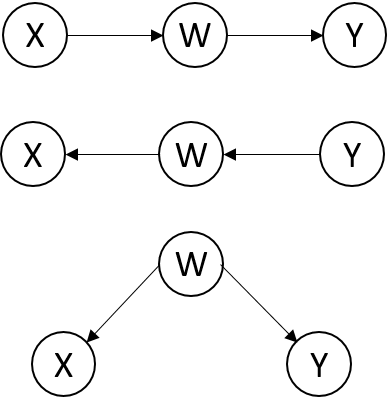
\includegraphics[width=\textwidth]{../figures/statisticalModeling/d-separationScheme}
		\caption{$X$ and $Y$ are d-separated by $W$}
	\end{subfigure}\quad
	\begin{subfigure}[b]{0.3\textwidth}
		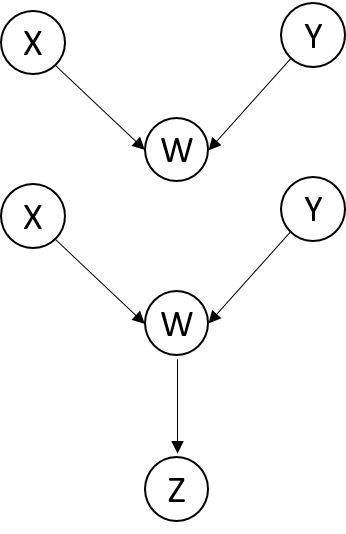
\includegraphics[width=\textwidth]{../figures/statisticalModeling/d-separationSchemeVstructure}
		\caption{$X$ and $Y$ are not d-separated by $W$ and $Z$.}
	\end{subfigure}
	\caption{d-separation examples.}
	\label{ch:statistical-models:fig:d-SeparationExamples}
\end{figure}


\begin{theorem}[d-sepration and conditional independence]
In a directed acyclic graphic model, $X$ is conditional independent from $Y$ given $\cV$ if $\cV$ d-separates $X$ from $Y$.	
\end{theorem}





\begin{theorem}[factorization theorem]\index{factorization theorem}
	If graph $G$ is an I-map of $P$, then
	$$P(X_1...X_n) = \prod_{i}^n P(X_i|Pa(X_i))$$
\end{theorem}
\begin{proof}
	by the chain rule lemma, we have
	$$P(X_1...X_n) = \prod_{i}^n P(X_i|X_1...X_i))$$
\end{proof}


\begin{example}	Consider the following graph models in ch:statistical-models:fig:graphModelExamples.
\begin{itemize}
	\item  For graphical model (A), we can have the following factorization
	$$P(A,B,C,D,E) = P(A)P(B)P(C|A,B)P(D|B,C)P(E|C,D).$$
	\item Consider the graphical model (B). A data set of $N$ points are generated iid from a Gaussian distribution with parameters $\mu$ and $\sigma$. The joint probability is given by
	$$P(X_1,X_2,...,X_N, \mu,\sigma) = P(\mu)P(\sigma) \prod_{n=1}^{N}P(X_n|\mu,\sigma).$$
	\item Consider the graphical model (C) representing a Markov chain.  The joint probability can be decomposed by
		$$P(X_1,X_2,...,X_N) = P(X_N|X_{N-1})P(X_{N-1}|X_{N-2})\cdots P(X_1).$$
	\item Consider the graphical model (D) representing a second-order Markov chain.  The joint probability can be decomposed by
	\begin{align*}
	&P(X_1,X_2,...,X_N) \\
	&= P(X_N|X_{N-1},X_{N-2})P(X_{N-1}|X_{N-2},X_{N-3})\cdots P(X_3|X_1,X_2)P(X_1)P(X_2).
	\end{align*}
	\item Consider the graphical model (E) representing a hidden Markov chain.  The joint probability can be decomposed by
	\begin{align*}
	&P(X_1,...,X_N,Z_1,...,Z_N) \\
	&= P(Z_{N}|Z_{N-1})P(Z_{N-1}|Z_{N-2})\cdots P(Z_1) \prod_{n=1}^N P(X_i|Z_i).
	\end{align*}
\end{itemize}	
\end{example}



\begin{figure}[H]
	\centering
	\begin{subfigure}[b]{0.3\textwidth}
		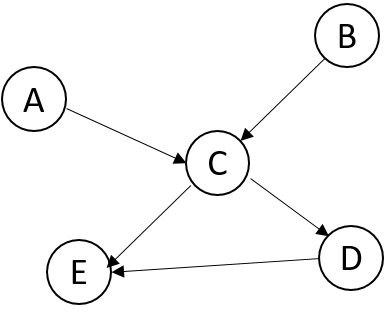
\includegraphics[width=\textwidth]{../figures/statisticalModeling/graphModelExample}
		\caption{Graphicial model A.}
	\end{subfigure}\quad
	\begin{subfigure}[b]{0.3\textwidth}
		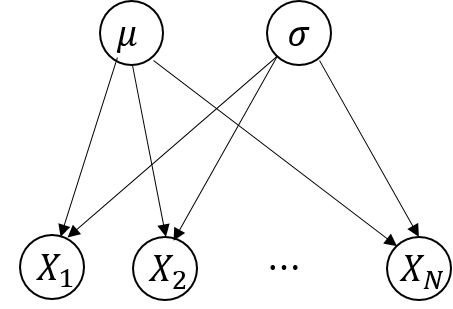
\includegraphics[width=\textwidth]{../figures/statisticalModeling/graphModelExample2}
		\caption{Graphicial model B. $\mu,\sigma$ are model parameters.}
	\end{subfigure}\quad
		\begin{subfigure}[b]{0.4\textwidth}
			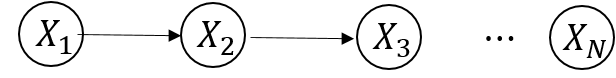
\includegraphics[width=\textwidth]{../figures/statisticalModeling/graphModelExample3}
			\caption{Graphical model C for a Markov chain model.}
		\end{subfigure}\\
		\begin{subfigure}[b]{0.5\textwidth}
			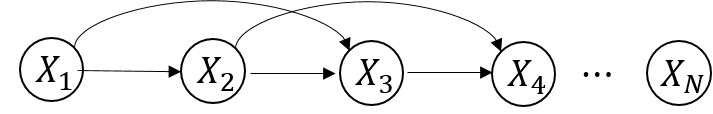
\includegraphics[width=\textwidth]{../figures/statisticalModeling/graphModelExample4}
			\caption{Graphical model D for a second-order Markov chain model.}
		\end{subfigure}\\
		\begin{subfigure}[b]{0.45\textwidth}
			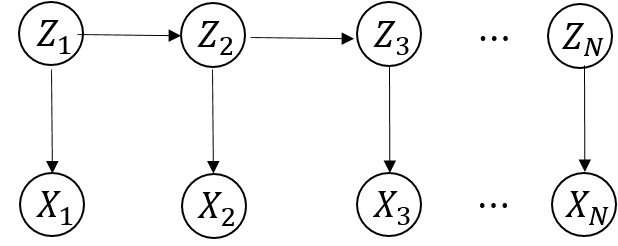
\includegraphics[width=\textwidth]{../figures/statisticalModeling/graphModelExample5}
			\caption{Graphical model E for a hidden Markov chain model.}
		\end{subfigure}
	\caption{Graphical model examples.}
	\label{ch:statistical-models:fig:graphModelExamples}
\end{figure}


\begin{example}[efficient inference via factorization]
Consider a joint distribution on random variables $A,B,C,D,E$ has the following factorization given by
	$$P(A,B,C,D,E) = P(A)P(B)P(C|A,B)P(D|B,C)P(E|C,D).$$

To calculate $$P(A|C=c) = \frac{P(A,C=c)}{P(C=c)},$$
we have
\begin{align*}
P(A,C=c) &= \sum_{B,D,E} P(A)P(B)P(C=c|A,B)P(D|B,C=c)P(E|C=c,D) \\
&=\sum_{B} P(A)P(B)P(C=c|A,B)\sum_{D}P(D|B,C=c)\sum_{E}P(E|C=c,D) \\
&=\sum_{B} P(A)P(B)P(C=c|A,B) 
\end{align*}		
	
\end{example}

\subsection{Undirected graphical model}


\begin{theorem}[Hammersley-Clifford theorem, fundamental theorem of random fields]\index{Hammersley-Clifford theorem}\index{fundamental theorem of random fields}
	A positive distribution $P >0$ satisfies the conditional independence of an undirected graph $G$ if and only if $P$ can be represented as a product of factors, one per maximal clique, such that
	$$p(\cX|\theta) = \frac{1}{Z(\theta)}\prod_{c\in \cC} \phi_c(\cX_c|\theta_c)$$
	where $\cC$ is the set of all the maximal cliques of $G$, and $Z(\theta)$ is the partition function given by 
	$$Z(\theta) = \int \prod_{c\in \cC}\phi_c(\cX_c|\theta_c) dP(\cX)$$
\end{theorem}


\begin{remark}
	This theorem guarantee that a distribution $P$ can be factored as distributions on cliques on the graph.
\end{remark}




see \cite{ankan2015mastering}
Risk Assessment and Decision Analysis with Bayesian Networks


\subsubsection{Correlation vs. causation}\index{correlation vs. causation}
\begin{remark}\hfill
	\begin{itemize}
		\item causation will imply correlation.
		\item correlation will \textbf{not} imply causation.
	\end{itemize}
	
For any two correlated events, A and B, the following relationships are possible:
\begin{itemize}
	\item A causes B; (direct causation)
	\item B causes A; (reverse causation)
	\item A and B are \textbf{consequences of a common cause of C}, but do not cause each other; graphically, we have $A\leftarrow C \rightarrow B$;
	\item A causes B and B causes A (bidirectional or cyclic causation);
	\item A causes C which causes B (indirect causation); graphically, we have $A\rightarrow C \rightarrow B$;
\end{itemize}	

	The Bayesian network assumes causation relations. Markov random field assumes correlation relations.	
\end{remark}






\section{Notes on Bibliography}

For linear regression models, see \cite{kutner2003applied}\cite{seber2012linear}. For, linear models with $R$ resources, see \cite{faraway2014linear}.


For multivariate statistical analysis, see \cite{johnson2007applied}\cite{anderson2009introduction}.

For copula, see \cite{Ruschendorf2013mathematical}\cite{lindskog2000modelling}\cite{mcneil2015quantitative}\cite{cherubini2004copula}.

\printbibliography
\end{refsection}
